
\begin{frame}{XPath}
XPath est un langage de requ\^etes
\begin{itemize}
\item non XML,
\item permettant l'accès \`a des parties d’une donn\'ee XML via l'expression de chemin menant \`a un ensemble de n{\oe}uds (sous-arbres) d'un document XML.
\end{itemize}

\medskip

XPath est utilis\'e dans 
\begin{description}
\item[XQuery] XPath fait partie du langage d’interrogation XQuery,
\item[XSLT] pour la s\'election de la partie des donn\'ees \`a transformer,
\item[XML Schema] pour les expressions de contraintes d’unicit\'e,
%\item[XSL] pour la s\'elections des parties des donn\'ees \`a formater,
\item[XPointer] pour l'identification de fragments,
\item[XLink] pour ancrer les liens hypertextes,
\item[...]
\end{description}
\end{frame}



\begin{frame}{XPath}

\begin{itemize}
\item XPath 1.0 est utilis\'e dans XSLT 1.0 (que nous \'etudierons dans ce cours),
\item XPath 1.0 est inclus dans XPath 2.0,
\item XPath 2.0 est inclus dans XQuery (que nous \'etudierons dans ce cours).
\end{itemize}

Nous commen\c{c}ons donc tout naturellement par \'etudier XPath 1.0.
\end{frame}


\subsection{Les chemins de localisation}

\begin{frame}{Une intuition}

Permet de ``pointer'' (localiser) des sous-arbres d'un document XML.

\begin{exampleblock}{Intuition}
Par navigation : en navigant dans l'arbre de "pas en pas" \`a partir de la racine, on va chercher \`a atteindre certaines de ses parties.
\end{exampleblock}

\end{frame}

\begin{frame}[allowframebreaks]{Commen\c{c}ons par un exemple}

\begin{center}
\begin{minipage}{0.7\textwidth}
\lstinputlisting[basicstyle=\tiny, language=XML,breaklines=true, caption={Un simple fichier XML}]{codes/livresExXpath.xml}
\end{minipage}
\end{center}

\framebreak

\texttt{/child::library/child::book/child::author}

\begin{center}
\begin{tikzpicture}[auto]
\tiny
  \tikzstyle{emptyStyle}=[text width=0.9cm, text centered]
  \tikzstyle{parser}=[rounded corners=3mm,thick,draw=DarkViolet!75,fill=DarkViolet!20,,text centered]
  \tikzstyle{appli}=[rounded corners=1mm,thick,draw=red!75,fill=red!20,text centered,text width=2cm]
  \tikzstyle{every label}=[black]

  \begin{scope}
    \node[emptyStyle](r) at (6,5) {Root};
   \node[emptyStyle](comment) at (1,4) {\texttt{\verb?<!-- ceci ... >?}};
   \draw[-] (r) -- (comment);
    %\node[emptyStyle](entete) at (3,4) {\texttt{$<?xml$ version $...>$}};
   %\draw[-] (r) -- (entete);
    \node[emptyStyle](library) at (6,4) {\verb?<library> ... </library>?};
   \draw[-] (r) -- (library);

    \node[emptyStyle](book1) at (3,3) {\verb?<book> ... </book>?};
   \draw[-] (library) -- (book1);
    \node[emptyStyle](book2) at (6,3) {\verb?<book> ... </book>?};
   \draw[-] (library) -- (book2);
    \node[emptyStyle](book3) at (10,3) {\verb?<book> ... </book>?};
   \draw[-] (library) -- (book3);

    \node[emptyStyle](year1) at (2,3) {\verb?year = "1857"?};
   \draw[-] (book1) -- (year1);
    \node[emptyStyle](author1) at (2,2) {\verb?<author> ... </author>?};
   \draw[-] (book1) -- (author1);
    \node[emptyStyle](textauthor1) at (2,1) {\it Charles Baudelaire};
   \draw[-] (author1) -- (textauthor1);
    \node[emptyStyle](title1) at (3,2) {\verb?<title> ... </title>?};
   \draw[-] (book1) -- (title1);
    \node[emptyStyle](texttitle1) at (3,1) {\it Les fleurs du mal};
   \draw[-] (title1) -- (texttitle1);

    \node[emptyStyle](year2) at (5,3) {\verb?year = "1862"?};
   \draw[-] (book2) -- (year2);
    \node[emptyStyle](author2) at (6,2) {\verb?<author> ... </author>?};
   \draw[-] (book2) -- (author2);
    \node[emptyStyle](textauthor2) at (6,1) {\it Victor Hugo};
   \draw[-] (author2) -- (textauthor2);
    \node[emptyStyle](ln2) at (5,2) {\verb?ln = "Besancon"?};
   \draw[-] (author2) -- (ln2);
    \node[emptyStyle](title2) at (7,2) {\verb?<title> ... </title>?};
   \draw[-] (book2) -- (title2);
    \node[emptyStyle](texttitle2) at (7,1) {\it Les miserables};
   \draw[-] (title2) -- (texttitle2);

    \node[emptyStyle](year3) at (9,3) {\verb?year = "1877"?};
   \draw[-] (book3) -- (year3);
    \node[emptyStyle](author3) at (10,2) {\verb?<author> ... </author>?};
   \draw[-] (book3) -- (author3);
    \node[emptyStyle](textauthor3) at (10,1) {\it Emile Zola};
   \draw[-] (author3) -- (textauthor3);
    \node[emptyStyle](ln3) at (9,2) {\verb?ln = "Paris"?};
   \draw[-] (author3) -- (ln3);
    \node[emptyStyle](title3) at (11,2) {\verb?<title> ... </title>?};
   \draw[-] (book3) -- (title3);
    \node[emptyStyle](texttitle3) at (11,1) {\it L'assomoir};
   \draw[-] (title3) -- (texttitle3);

\end{scope}

%  \begin{pgfonlayer}{background}
%    \filldraw [line width=4mm,join=round,black!20]
%      (parser.north  -| parser.west)  rectangle (serial.south  -| serial.east);
%\end{pgfonlayer}


\end{tikzpicture}
\end{center}

\framebreak

\texttt{\textcolor{red}{\bf /}child::library/child::book/child::author}

\begin{center}
\begin{tikzpicture}[auto]
\tiny
  \tikzstyle{emptyStyle}=[text width=0.9cm, text centered]
  \tikzstyle{red}=[rounded corners=1mm,thick,draw=red!75,fill=red!20,text width=0.9cm, text centered]
  \tikzstyle{DarkViolet}=[rounded corners=1mm,thick,draw=DarkViolet!75,fill=DarkViolet!20,minimum size=7mm,text width=0.8cm, text centered]
 \tikzstyle{every label}=[black]

  \begin{scope}
    \node[red](r) at (6,5) {Root};
   \node[emptyStyle](comment) at (1,4) {\texttt{\verb?<!-- ceci ... >?}};
   \draw[-] (r) -- (comment);
    %\node[emptyStyle](entete) at (3,4) {\texttt{$<?xml$ version $...>$}};
   %\draw[-] (r) -- (entete);
    \node[emptyStyle](library) at (6,4) {\verb?<library> ... </library>?};
   \draw[-] (r) -- (library);

    \node[emptyStyle](book1) at (3,3) {\verb?<book> ... </book>?};
   \draw[-] (library) -- (book1);
    \node[emptyStyle](book2) at (6,3) {\verb?<book> ... </book>?};
   \draw[-] (library) -- (book2);
    \node[emptyStyle](book3) at (10,3) {\verb?<book> ... </book>?};
   \draw[-] (library) -- (book3);

    \node[emptyStyle](year1) at (2,3) {\verb?year = "1857"?};
   \draw[-] (book1) -- (year1);
    \node[emptyStyle](author1) at (2,2) {\verb?<author> ... </author>?};
   \draw[-] (book1) -- (author1);
    \node[emptyStyle](textauthor1) at (2,1) {\it Charles Baudelaire};
   \draw[-] (author1) -- (textauthor1);
    \node[emptyStyle](title1) at (3,2) {\verb?<title> ... </title>?};
   \draw[-] (book1) -- (title1);
    \node[emptyStyle](texttitle1) at (3,1) {\it Les fleurs du mal};
   \draw[-] (title1) -- (texttitle1);

    \node[emptyStyle](year2) at (5,3) {\verb?year = "1862"?};
   \draw[-] (book2) -- (year2);
    \node[emptyStyle](author2) at (6,2) {\verb?<author> ... </author>?};
   \draw[-] (book2) -- (author2);
    \node[emptyStyle](textauthor2) at (6,1) {\it Victor Hugo};
   \draw[-] (author2) -- (textauthor2);
    \node[emptyStyle](ln2) at (5,2) {\verb?ln = "Besancon"?};
   \draw[-] (author2) -- (ln2);
    \node[emptyStyle](title2) at (7,2) {\verb?<title> ... </title>?};
   \draw[-] (book2) -- (title2);
    \node[emptyStyle](texttitle2) at (7,1) {\it Les miserables};
   \draw[-] (title2) -- (texttitle2);

    \node[emptyStyle](year3) at (9,3) {\verb?year = "1877"?};
   \draw[-] (book3) -- (year3);
    \node[emptyStyle](author3) at (10,2) {\verb?<author> ... </author>?};
   \draw[-] (book3) -- (author3);
    \node[emptyStyle](textauthor3) at (10,1) {\it Emile Zola};
   \draw[-] (author3) -- (textauthor3);
    \node[emptyStyle](ln3) at (9,2) {\verb?ln = "Paris"?};
   \draw[-] (author3) -- (ln3);
    \node[emptyStyle](title3) at (11,2) {\verb?<title> ... </title>?};
   \draw[-] (book3) -- (title3);
    \node[emptyStyle](texttitle3) at (11,1) {\it L'assomoir};
   \draw[-] (title3) -- (texttitle3);

\end{scope}

%  \begin{pgfonlayer}{background}
%    \filldraw [line width=4mm,join=round,black!20]
%      (parser.north  -| parser.west)  rectangle (serial.south  -| serial.east);
%\end{pgfonlayer}


\end{tikzpicture}
\end{center}


\framebreak

\texttt{\textcolor{red}{\bf /}\textcolor{DarkViolet}{\bf child::library}/child::book/child::author}

\begin{center}
\begin{tikzpicture}[auto]
\tiny
  \tikzstyle{emptyStyle}=[text width=0.9cm, text centered]
  \tikzstyle{red}=[rounded corners=1mm,thick,draw=red!75,fill=red!20,text width=0.9cm, text centered]
  \tikzstyle{DarkViolet}=[rounded corners=1mm,thick,draw=DarkViolet!75,fill=DarkViolet!20,minimum size=7mm,text width=0.8cm, text centered]
 \tikzstyle{every label}=[black]

  \begin{scope}
    \node[red](r) at (6,5) {Root};
   \node[emptyStyle](comment) at (1,4) {\texttt{\verb?<!-- ceci ... >?}};
   \draw[-] (r) -- (comment);
    %\node[emptyStyle](entete) at (3,4) {\texttt{$<?xml$ version $...>$}};
   %\draw[-] (r) -- (entete);
    \node[DarkViolet](library) at (6,4) {\verb?<library> ... </library>?};
   \draw[-] (r) -- (library);

    \node[emptyStyle](book1) at (3,3) {\verb?<book> ... </book>?};
   \draw[-] (library) -- (book1);
    \node[emptyStyle](book2) at (6,3) {\verb?<book> ... </book>?};
   \draw[-] (library) -- (book2);
    \node[emptyStyle](book3) at (10,3) {\verb?<book> ... </book>?};
   \draw[-] (library) -- (book3);

    \node[emptyStyle](year1) at (2,3) {\verb?year = "1857"?};
   \draw[-] (book1) -- (year1);
    \node[emptyStyle](author1) at (2,2) {\verb?<author> ... </author>?};
   \draw[-] (book1) -- (author1);
    \node[emptyStyle](textauthor1) at (2,1) {\it Charles Baudelaire};
   \draw[-] (author1) -- (textauthor1);
    \node[emptyStyle](title1) at (3,2) {\verb?<title> ... </title>?};
   \draw[-] (book1) -- (title1);
    \node[emptyStyle](texttitle1) at (3,1) {\it Les fleurs du mal};
   \draw[-] (title1) -- (texttitle1);

    \node[emptyStyle](year2) at (5,3) {\verb?year = "1862"?};
   \draw[-] (book2) -- (year2);
    \node[emptyStyle](author2) at (6,2) {\verb?<author> ... </author>?};
   \draw[-] (book2) -- (author2);
    \node[emptyStyle](textauthor2) at (6,1) {\it Victor Hugo};
   \draw[-] (author2) -- (textauthor2);
    \node[emptyStyle](ln2) at (5,2) {\verb?ln = "Besancon"?};
   \draw[-] (author2) -- (ln2);
    \node[emptyStyle](title2) at (7,2) {\verb?<title> ... </title>?};
   \draw[-] (book2) -- (title2);
    \node[emptyStyle](texttitle2) at (7,1) {\it Les miserables};
   \draw[-] (title2) -- (texttitle2);

    \node[emptyStyle](year3) at (9,3) {\verb?year = "1877"?};
   \draw[-] (book3) -- (year3);
    \node[emptyStyle](author3) at (10,2) {\verb?<author> ... </author>?};
   \draw[-] (book3) -- (author3);
    \node[emptyStyle](textauthor3) at (10,1) {\it Emile Zola};
   \draw[-] (author3) -- (textauthor3);
    \node[emptyStyle](ln3) at (9,2) {\verb?ln = "Paris"?};
   \draw[-] (author3) -- (ln3);
    \node[emptyStyle](title3) at (11,2) {\verb?<title> ... </title>?};
   \draw[-] (book3) -- (title3);
    \node[emptyStyle](texttitle3) at (11,1) {\it L'assomoir};
   \draw[-] (title3) -- (texttitle3);

\end{scope}

%  \begin{pgfonlayer}{background}
%    \filldraw [line width=4mm,join=round,black!20]
%      (parser.north  -| parser.west)  rectangle (serial.south  -| serial.east);
%\end{pgfonlayer}


\end{tikzpicture}
\end{center}

\framebreak

\texttt{\textcolor{red}{\bf /}\textcolor{DarkViolet}{\bf child::library}\textcolor{DarkOliveGreen}{\bf /child::book}/child::author}

\begin{center}
\begin{tikzpicture}[auto]
\tiny
  \tikzstyle{emptyStyle}=[text width=0.9cm, text centered]
  \tikzstyle{red}=[rounded corners=1mm,thick,draw=red!75,fill=red!20,text width=0.9cm, text centered]
  \tikzstyle{DarkViolet}=[rounded corners=1mm,thick,draw=DarkViolet!75,fill=DarkViolet!20,minimum size=7mm,text width=0.8cm, text centered]
  \tikzstyle{green}=[rounded corners=1mm,thick,draw=DarkOliveGreen!75,fill=DarkOliveGreen!20,minimum size=7mm,text width=0.8cm, text centered]
 \tikzstyle{every label}=[black]

  \begin{scope}
    \node[red](r) at (6,5) {Root};
   \node[emptyStyle](comment) at (1,4) {\texttt{\verb?<!-- ceci ... >?}};
   \draw[-] (r) -- (comment);
    %\node[emptyStyle](entete) at (3,4) {\texttt{$<?xml$ version $...>$}};
   %\draw[-] (r) -- (entete);
    \node[DarkViolet](library) at (6,4) {\verb?<library> ... </library>?};
   \draw[-] (r) -- (library);

    \node[green](book1) at (3,3) {\verb?<book> ... </book>?};
   \draw[-] (library) -- (book1);
    \node[green](book2) at (6,3) {\verb?<book> ... </book>?};
   \draw[-] (library) -- (book2);
    \node[green](book3) at (10,3) {\verb?<book> ... </book>?};
   \draw[-] (library) -- (book3);

    \node[emptyStyle](year1) at (2,3) {\verb?year = "1857"?};
   \draw[-] (book1) -- (year1);
    \node[emptyStyle](author1) at (2,2) {\verb?<author> ... </author>?};
   \draw[-] (book1) -- (author1);
    \node[emptyStyle](textauthor1) at (2,1) {\it Charles Baudelaire};
   \draw[-] (author1) -- (textauthor1);
    \node[emptyStyle](title1) at (3,2) {\verb?<title> ... </title>?};
   \draw[-] (book1) -- (title1);
    \node[emptyStyle](texttitle1) at (3,1) {\it Les fleurs du mal};
   \draw[-] (title1) -- (texttitle1);

    \node[emptyStyle](year2) at (5,3) {\verb?year = "1862"?};
   \draw[-] (book2) -- (year2);
    \node[emptyStyle](author2) at (6,2) {\verb?<author> ... </author>?};
   \draw[-] (book2) -- (author2);
    \node[emptyStyle](textauthor2) at (6,1) {\it Victor Hugo};
   \draw[-] (author2) -- (textauthor2);
    \node[emptyStyle](ln2) at (5,2) {\verb?ln = "Besancon"?};
   \draw[-] (author2) -- (ln2);
    \node[emptyStyle](title2) at (7,2) {\verb?<title> ... </title>?};
   \draw[-] (book2) -- (title2);
    \node[emptyStyle](texttitle2) at (7,1) {\it Les miserables};
   \draw[-] (title2) -- (texttitle2);

    \node[emptyStyle](year3) at (9,3) {\verb?year = "1877"?};
   \draw[-] (book3) -- (year3);
    \node[emptyStyle](author3) at (10,2) {\verb?<author> ... </author>?};
   \draw[-] (book3) -- (author3);
    \node[emptyStyle](textauthor3) at (10,1) {\it Emile Zola};
   \draw[-] (author3) -- (textauthor3);
    \node[emptyStyle](ln3) at (9,2) {\verb?ln = "Paris"?};
   \draw[-] (author3) -- (ln3);
    \node[emptyStyle](title3) at (11,2) {\verb?<title> ... </title>?};
   \draw[-] (book3) -- (title3);
    \node[emptyStyle](texttitle3) at (11,1) {\it L'assomoir};
   \draw[-] (title3) -- (texttitle3);

\end{scope}

%  \begin{pgfonlayer}{background}
%    \filldraw [line width=4mm,join=round,black!20]
%      (parser.north  -| parser.west)  rectangle (serial.south  -| serial.east);
%\end{pgfonlayer}


\end{tikzpicture}
\end{center}


\framebreak

\texttt{\textcolor{red}{\bf /}\textcolor{DarkViolet}{\bf child::library}\textcolor{DarkOliveGreen}{\bf /child::book}\textcolor{DarkCyan}{\bf  /child::author}}


\begin{center}
\begin{tikzpicture}[auto]
\tiny
  \tikzstyle{emptyStyle}=[text width=0.9cm, text centered]
  \tikzstyle{red}=[rounded corners=1mm,thick,draw=red!75,fill=red!20,text width=0.9cm, text centered]
  \tikzstyle{DarkViolet}=[rounded corners=1mm,thick,draw=DarkViolet!75,fill=DarkViolet!20,minimum size=7mm,text width=0.8cm, text centered]
  \tikzstyle{green}=[rounded corners=1mm,thick,draw=DarkOliveGreen!75,fill=DarkOliveGreen!20,minimum size=7mm,text width=0.8cm, text centered]
  \tikzstyle{cyan}=[rounded corners=1mm,thick,draw=DarkCyan!75,fill=DarkCyan!20,minimum size=7mm,text width=0.8cm, text centered]
 \tikzstyle{every label}=[black]

  \begin{scope}
    \node[red](r) at (6,5) {Root};
   \node[emptyStyle](comment) at (1,4) {\texttt{\verb?<!-- ceci ... >?}};
   \draw[-] (r) -- (comment);
    %\node[emptyStyle](entete) at (3,4) {\texttt{$<?xml$ version $...>$}};
   %\draw[-] (r) -- (entete);
    \node[DarkViolet](library) at (6,4) {\verb?<library> ... </library>?};
   \draw[-] (r) -- (library);

    \node[green](book1) at (3,3) {\verb?<book> ... </book>?};
   \draw[-] (library) -- (book1);
    \node[green](book2) at (6,3) {\verb?<book> ... </book>?};
   \draw[-] (library) -- (book2);
    \node[green](book3) at (10,3) {\verb?<book> ... </book>?};
   \draw[-] (library) -- (book3);

    \node[emptyStyle](year1) at (2,3) {\verb?year = "1857"?};
   \draw[-] (book1) -- (year1);
    \node[cyan](author1) at (2,2) {\verb?<author> ... </author>?};
   \draw[-] (book1) -- (author1);
    \node[emptyStyle](textauthor1) at (2,1) {\it Charles Baudelaire};
   \draw[-] (author1) -- (textauthor1);
    \node[emptyStyle](title1) at (3,2) {\verb?<title> ... </title>?};
   \draw[-] (book1) -- (title1);
    \node[emptyStyle](texttitle1) at (3,1) {\it Les fleurs du mal};
   \draw[-] (title1) -- (texttitle1);

    \node[emptyStyle](year2) at (5,3) {\verb?year = "1862"?};
   \draw[-] (book2) -- (year2);
    \node[cyan](author2) at (6,2) {\verb?<author> ... </author>?};
   \draw[-] (book2) -- (author2);
    \node[emptyStyle](textauthor2) at (6,1) {\it Victor Hugo};
   \draw[-] (author2) -- (textauthor2);
    \node[emptyStyle](ln2) at (5,2) {\verb?ln = "Besancon"?};
   \draw[-] (author2) -- (ln2);
    \node[emptyStyle](title2) at (7,2) {\verb?<title> ... </title>?};
   \draw[-] (book2) -- (title2);
    \node[emptyStyle](texttitle2) at (7,1) {\it Les miserables};
   \draw[-] (title2) -- (texttitle2);

    \node[emptyStyle](year3) at (9,3) {\verb?year = "1877"?};
   \draw[-] (book3) -- (year3);
    \node[cyan](author3) at (10,2) {\verb?<author> ... </author>?};
   \draw[-] (book3) -- (author3);
    \node[emptyStyle](textauthor3) at (10,1) {\it Emile Zola};
   \draw[-] (author3) -- (textauthor3);
    \node[emptyStyle](ln3) at (9,2) {\verb?ln = "Paris"?};
   \draw[-] (author3) -- (ln3);
    \node[emptyStyle](title3) at (11,2) {\verb?<title> ... </title>?};
   \draw[-] (book3) -- (title3);
    \node[emptyStyle](texttitle3) at (11,1) {\it L'assomoir};
   \draw[-] (title3) -- (texttitle3);

\end{scope}

%  \begin{pgfonlayer}{background}
%    \filldraw [line width=4mm,join=round,black!20]
%      (parser.north  -| parser.west)  rectangle (serial.south  -| serial.east);
%\end{pgfonlayer}


\end{tikzpicture}
\end{center}

\end{frame}



\begin{frame}{L'arbre XML vu par XPath}

\begin{center}
\begin{tikzpicture}[auto]
\tiny
  \tikzstyle{emptyStyle}=[text width=0.9cm, text centered]
  \tikzstyle{red}=[rounded corners=1mm,thick,draw=red!75,fill=red!20,text width=0.9cm, text centered]
  \tikzstyle{DarkViolet}=[rounded corners=1mm,thick,draw=DarkViolet!75,fill=DarkViolet!20,minimum size=7mm,text width=0.8cm, text centered]
  \tikzstyle{green}=[rounded corners=1mm,thick,draw=DarkOliveGreen!75,fill=DarkOliveGreen!20,minimum size=7mm,text width=0.8cm, text centered]
  \tikzstyle{cyan}=[rounded corners=1mm,thick,draw=DarkCyan!75,fill=DarkCyan!20,minimum size=7mm,text width=0.8cm, text centered]
 \tikzstyle{every label}=[black]
  \tikzstyle{HotPink}=[rounded corners=1mm,thick,draw=HotPink!75,fill=HotPink!20,minimum size=7mm,text width=0.8cm, text centered]
  \tikzstyle{Olive}=[rounded corners=1mm,thick,draw=Olive!75,fill=Olive!20,minimum size=7mm,text width=0.9cm, text centered]
  \tikzstyle{indiaRed}=[rounded corners=1mm,thick,draw=indiaRed!75,fill=indiaRed!20,minimum size=7mm,text width=0.9cm, text centered]

  \begin{scope}
    \node[red](r) at (6,5) {Root};  
    \node[emptyStyle,text width=1cm](rootnode) at (9,5) {\textcolor{red}{\textit{Root node} (pas un \textit{element node})}};  
   \draw[->,dashed,draw=red] (rootnode) -- (r);
   \node[indiaRed, label={\textcolor{indiaRed}{\textit{Comment node}}}](comment) at (1,4) {\texttt{\verb?<!-- ceci ... >?}};
   \draw[-] (r) -- (comment);
    %\node[emptyStyle](entete) at (3,4) {\texttt{$<?xml$ version $...>$}};
   %\draw[-] (r) -- (entete);
    \node[emptyStyle,text width=1cm](elementnode) at (10,4) {\textcolor{HotPink}{\textit{Element nodes}}};  
    \node[HotPink](library) at (6,4) {\verb?<library> ... </library>?};
   \draw[-] (r) -- (library);
   \draw[->,dashed,draw=HotPink] (elementnode) -- (library);

    \node[HotPink](book1) at (3,3) {\verb?<book> ... </book>?};
   \draw[-] (library) -- (book1);
   \draw[->,dashed,draw=HotPink] (elementnode) -- (book1);
    \node[HotPink](book2) at (6,3) {\verb?<book> ... </book>?};
   \draw[-] (library) -- (book2);
   \draw[->,dashed,draw=HotPink] (elementnode) -- (book2);
    \node[HotPink](book3) at (10,3) {\verb?<book> ... </book>?};
   \draw[-] (library) -- (book3);

    \node[cyan](year1) at (2,3) {\verb?year = "1857"?};
   \draw[-] (book1) -- (year1);
    \node[HotPink](author1) at (2,2) {\verb?<author> ... </author>?};
   \draw[-] (book1) -- (author1);
    \node[Olive](textauthor1) at (2,1) {\it Charles Baudelaire};
   \draw[-] (author1) -- (textauthor1);
    \node[HotPink](title1) at (3,2) {\verb?<title> ... </title>?};
   \draw[-] (book1) -- (title1);
    \node[Olive](texttitle1) at (3,1) {\it Les fleurs du mal};
   \draw[-] (title1) -- (texttitle1);

    \node[cyan](year2) at (5,3) {\verb?year = "1862"?};
   \draw[-] (book2) -- (year2);
    \node[HotPink](author2) at (6,2) {\verb?<author> ... </author>?};
   \draw[-] (book2) -- (author2);
    \node[Olive](textauthor2) at (6,1) {\it Victor Hugo};
   \draw[-] (author2) -- (textauthor2);
    \node[cyan](ln2) at (5,2) {\verb?ln = "Besancon"?};
   \draw[-] (author2) -- (ln2);
    \node[HotPink](title2) at (7,2) {\verb?<title> ... </title>?};
   \draw[-] (book2) -- (title2);
    \node[Olive](texttitle2) at (7,1) {\it Les miserables};
   \draw[-] (title2) -- (texttitle2);


    \node[cyan](year3) at (9,3) {\verb?year = "1877"?};
   \draw[-] (book3) -- (year3);
    \node[HotPink](author3) at (10,2) {\verb?<author> ... </author>?};
   \draw[-] (book3) -- (author3);
    \node[Olive](textauthor3) at (10,1) {\it Emile Zola};
   \draw[-] (author3) -- (textauthor3);
    \node[cyan](ln3) at (9,2) {\verb?ln = "Paris"?};
   \draw[-] (author3) -- (ln3);
    \node[HotPink](title3) at (11,2) {\verb?<title> ... </title>?};
   \draw[-] (book3) -- (title3);
    \node[Olive](texttitle3) at (11,1) {\it L'assomoir};
   \draw[-] (title3) -- (texttitle3);
    \node[emptyStyle,text width=1cm](textnode) at (4,0) {\textcolor{Olive}{\textit{Text nodes}}};  
   \draw[->,dashed,draw=Olive] (textnode) -- (textauthor1);
   \draw[->,dashed,draw=Olive] (textnode) -- (texttitle1);
   \draw[->,dashed,draw=Olive] (textnode) -- (textauthor2);
    \node[emptyStyle,text width=1cm](attnode) at (8,0) {\textcolor{cyan}{\textit{Attribute nodes}}};  
   \draw[->,dashed,draw=cyan] (attnode) -- (ln2);
   \draw[->,dashed,draw=cyan] (attnode) -- (ln3);
   \draw[->,dashed,draw=cyan] (attnode) -- (year3);
\end{scope}

%  \begin{pgfonlayer}{background}
%    \filldraw [line width=4mm,join=round,black!20]
%      (parser.north  -| parser.west)  rectangle (serial.south  -| serial.east);
%\end{pgfonlayer}

\end{tikzpicture}
\end{center}

+ \textit{Namespace nodes} + \textit{Processing instruction nodes} \prof{(que nous verrons plus loin dans le cours).}

NB : XPath ``ne voit pas'' le sch\'ema (doctype). \prof{cad qu'on ne peut pas l'interroger}

\end{frame}



\begin{frame}{L'arbre XML vu par XPath}

\begin{center}
\begin{tikzpicture}[auto]
\tiny
  \tikzstyle{emptyStyle}=[text width=0.9cm, text centered]
  \tikzstyle{red}=[rounded corners=1mm,thick,draw=red!75,fill=red!20,text width=0.9cm, text centered]
  \tikzstyle{DarkViolet}=[rounded corners=1mm,thick,draw=DarkViolet!75,fill=DarkViolet!20,minimum size=7mm,text width=0.8cm, text centered]
  \tikzstyle{green}=[rounded corners=1mm,thick,draw=DarkOliveGreen!75,fill=DarkOliveGreen!20,minimum size=7mm,text width=0.8cm, text centered]
  \tikzstyle{cyan}=[rounded corners=1mm,thick,draw=DarkCyan!75,fill=DarkCyan!20,minimum size=7mm,text width=0.8cm, text centered]
 \tikzstyle{every label}=[black]
  \tikzstyle{HotPink}=[rounded corners=1mm,thick,draw=HotPink!75,fill=HotPink!20,minimum size=7mm,text width=0.8cm, text centered]
  \tikzstyle{Olive}=[rounded corners=1mm,thick,draw=Olive!75,fill=Olive!20,minimum size=7mm,text width=0.9cm, text centered]
  \tikzstyle{indiaRed}=[rounded corners=1mm,thick,draw=indiaRed!75,fill=indiaRed!20,minimum size=7mm,text width=0.9cm, text centered]

  \begin{scope}
    \node[emptyStyle](r) at (6,5) {Root};  
  \node[emptyStyle](comment) at (1,4) {\texttt{\verb?<!-- ceci ... >?}};
   \draw[-] (r) -- node{\textcolor{orange}{\bf $\swarrow$ fils XPath}}   (comment);
    %\node[emptyStyle](entete) at (3,4) {\texttt{$<?xml$ version $...>$}};
   %\draw[-] (r) -- (entete);
   \node[emptyStyle](library) at (6,4) {\verb?<library> ... </library>?};
   \draw[-] (r) -- (library);

    \node[emptyStyle](book1) at (3,3) {\verb?<book> ... </book>?};
   \draw[-] (library) -- (book1);
   \node[emptyStyle](book2) at (6,3) {\verb?<book> ... </book>?};
   \draw[-] (library) -- (book2);
   \node[emptyStyle](book3) at (10,3) {\verb?<book> ... </book>?};
   \draw[-] (library) -- node{\textcolor{orange}{\bf $\searrow$ fils XPath}}   (book3);

    \node[emptyStyle](year1) at (2,3) {\verb?year = "1857"?};
   \draw[-] (book1) -- (year1);
    \node[emptyStyle](author1) at (2,2) {\verb?<author> ... </author>?};
   \draw[-] (book1) -- (author1);
    \node[emptyStyle](textauthor1) at (2,1) {\it Charles Baudelaire};
   \draw[-] (author1) -- (textauthor1);
    \node[emptyStyle](title1) at (3,2) {\verb?<title> ... </title>?};
   \draw[-] (book1) -- (title1);
    \node[emptyStyle](texttitle1) at (3,1) {\it Les fleurs du mal};
   \draw[-] (title1) -- (texttitle1);

    \node[emptyStyle](year2) at (5,3) {\verb?year = "1862"?};
   \draw[-] (book2) -- (year2);
    \node[emptyStyle](author2) at (6,2) {\verb?<author> ... </author>?};
   \draw[-] (book2) -- (author2);
    \node[emptyStyle](textauthor2) at (6,1) {\it Victor Hugo};
   \draw[-] (author2) -- (textauthor2);
    \node[emptyStyle](ln2) at (5,2) {\verb?ln = "Besancon"?};
   \draw[-] (author2) -- (ln2);
    \node[emptyStyle](title2) at (7,2) {\verb?<title> ... </title>?};
   \draw[-] (book2) -- (title2);
    \node[emptyStyle](texttitle2) at (7,1) {\it Les miserables};
   \draw[-] (title2) -- (texttitle2);


    \node[emptyStyle](year3) at (9,3) {\verb?year = "1877"?};
   \draw[-] (book3) -- (year3);
    \node[emptyStyle](author3) at (10,2) {\verb?<author> ... </author>?};
   \draw[-] (book3) -- (author3);
    \node[emptyStyle](textauthor3) at (10,1) {\it Emile Zola};
   \draw[-] (author3) -- (textauthor3);
    \node[emptyStyle](ln3) at (9,2) {\verb?ln = "Paris"?};
   \draw[-] (author3) -- (ln3);
    \node[emptyStyle](title3) at (11,2) {\verb?<title> ... </title>?};
   \draw[-] (book3) -- (title3);
    \node[emptyStyle](texttitle3) at (11,1) {\it L'assomoir};
   \draw[-] (title3) -- (texttitle3);


\end{scope}

\end{tikzpicture}
\end{center}

\medskip

$\Rightarrow$ Un fils au sens de XPath est différent d'un sous-\'el\'ement du mod\`ele de donn\'ees XML 
(\url{http://www.w3.org/TR/xpath-datamodel/})
\prof{un fils n'est pas forcément un sous-élément, ce peut être pas exemple un commentaire ou un attribut}

\end{frame}




\begin{frame}{Expression de chemin XPath (d\'efinition simplifi\'ee)}

Expression de chemin absolu (\'evalu\'ee à la racine) : 
\texttt{/\textcolor{DarkViolet}{step1}/\textcolor{DarkViolet}{step2}/\textcolor{DarkViolet}{step3}/…/\textcolor{DarkViolet}{stepN}}
\\

\medskip 

\noindent Chaque \texttt{\textcolor{DarkViolet}{stepi}} est une expression de la forme \\
\texttt{\textcolor{indiaRed}{axis}::\textcolor{DarkOliveGreen}{node-test}\textcolor{cyan}{[predicate]}
}\\
 o\`u

\begin{description}
\item[\texttt{\textcolor{indiaRed}{axis}}] est la direction du pas (\texttt{\textcolor{indiaRed}{child}}  par d\'efaut)\\
Ex : \texttt{\textcolor{indiaRed}{child}} ``descend'' sur les fils, \texttt{\textcolor{indiaRed}{attribut}} ``descend'' sur les attributs.
\item[\texttt{\textcolor{DarkOliveGreen}{node-test}}] est le type de nœud à retenir\\
Ex : \texttt{\textcolor{DarkOliveGreen}{book}} teste si l'\'el\'ement atteint (p.e. nœud ou attribut) est un \'el\'ement nomm\'e \texttt{book}.
Si \texttt{\textcolor{DarkOliveGreen}{*}},  tout nom.
\item[\texttt{\textcolor{cyan}{[predicate]}}] (optionnel) filtre les nœuds selon une expression bool\'eenne \\
	Ex : \texttt{\textcolor{cyan}{[attribute::supplier='store']}} teste si le nœud a un attribut supplier dont la valeur est \texttt{store}.\\
	Possibilit\'e d'utiliser des fonctions pr\'ed\'efinies dans XPath dans les pr\'edicats, par exemple : \texttt{\textcolor{cyan}{[position()=2]}} teste si le nœud est en seconde position, \texttt{\textcolor{cyan}{[position()=last()]}} teste si le nœud est en derni\`ere position.\\
\end{description}

\end{frame}

\begin{frame}{Quelques exemples simples: \`a vous de jouer...}

\vspace{-0.3cm}

\begin{footnotesize}

\lstinputlisting[basicstyle=\tiny, language=XML,breaklines=true, caption={Fichier limonade.xml}]{codes/limonade.xml}

\vspace{-0.3cm}

\begin{exoblock}

\'Evaluer (sur papier) les requêtes suivantes, sur le fichier limonade.xml se trouvant ci-dessus.

\noindent \texttt{1) /child::inventory \\
2) /child::inventory/child::drink \\
3) /child::inventory/child::drink/child::*\\
4) /child::inventory/child::drink/child::lemonade\\
5) /child::inventory/child::drink/child::*/child::price\\
6) /child::inventory/child::drink/child::price\\
}

Vous pourrez vérifier vos réponses, par exemple sur le site \url{http://www.zrinity.com/xml/xpath/} proposant un évaluateur de requêtes XPath en ligne.
\end{exoblock}
\end{footnotesize}

\prof{\`a faire en cours}
\end{frame}


\begin{frame}{Chemin de localisation : intuition}

\begin{block}{Intuition}
Un chemin de localisation XPath est une suite de mouvements (steps) , chaque mouvement \'etant \'eventuellement suivi de tests sur les n{\oe}uds atteints.
\end{block}

\medskip

Chaque \textit{pas} ``ram\`ene'' un ensemble de n{\oe}uds (de sous-arbres associés) à partir desquels est évalué le pas suivant. 

\end{frame}


\begin{frame}{Contexte d'évaluation}

Une expression de chemin est \'evalu\'ee par rapport \`a un \textit{contexte}.

\bigskip

Un contexte $[< N1,N2,...,Nn >,Nc]$ consiste en \cite{WDMD} :
\begin{itemize}
\item Une liste de n{\oe}uds $< N1,N2,...,Nn >$ de l'arbre XML
\item Un n{\oe}ud courant $Nc$ appartenant à la liste de n{\oe}ud
\end{itemize}

\medskip

\begin{block}{Concernant le contexte}
La taille du contexte $n$ indique la taille de la liste de n{\oe}uds. On peut la récupérer à l'aide de la fonction \verb?last()?;

\medskip

La position du n{\oe}ud contexte $c \in [1, n]$ indique la position du n{\oe}ud courant au sein de la liste de n{\oe}ud du contexte.
On peut la récupérer à l'aide de la fonction \verb?position()?.
\end{block}


\end{frame}


\begin{frame}[allowframebreaks]{Chemin de localisation : intuition}

\begin{center}
\figSized{images/evalxpath.jpg}{\'Evaluation d'une requ\^ete XPath}{0.6}
\end{center}


\framebreak
\cite{WDMD} Un pas $step_i$ est évalué par rapport au context produit par l'évaluation de $step_{i-1}$. 

\begin{description}
\item[Pour $i=1$ (premier pas)] si l'expression est absolue alors le contexte initial est $[<r>,r]$ où $r$ est le n{\oe}ud racine. Si l'expression est relative alors le contexte est défini par l'environnement.
\item[Pour $i > 1$] si $\mathcal{N} =< N1,N2,...,Nn >$ est le résultat de l'évaluation du pas $step_{i-1}$ alors $step_i$  est successivement évalué par rapport au context $[\mathcal{N},Nj]$, pour chaque $j \in [1,n]$.
\end{description}
Le résultat de l'évaluation est l'\textcolor{orange}{\textbf{ensemble}} de n{\oe}uds obtenu après l'évaluation du dernier pas.

\medskip

\`A un niveau de d\'etail plus fin, pour chaque pas de la forme \texttt{\textcolor{indiaRed}{axis}::\textcolor{DarkOliveGreen}{node-test}\textcolor{cyan}{[predicate]}}, le contexte passe (est transform\'e) successivement par l'axe (\texttt{\textcolor{indiaRed}{axis}}), puis le test de n{\oe}ud (\texttt{\textcolor{DarkOliveGreen}{node-test}}), puis le pr\'edicat (\texttt{\textcolor{cyan}{[predicate]}}). 

\end{frame}


\begin{frame}{Poussons la d\'efinition}

Il existe deux types de chemins de localisation : \\
\begin{description}
\item[chemin absolu] le r\'esultat de l'\'evaluation ne d\'epend pas du nœud contexte car l'expression est \'evalu\'ee \`a partir de la racine \\ \texttt{/\textcolor{DarkViolet}{step1}/\textcolor{DarkViolet}{step2}/\textcolor{DarkViolet}{step3}/…/\textcolor{DarkViolet}{stepN}}\\
\item[chemin relatif] le r\'esultat de l'\'evaluation d\'epend du nœud contexte  car l'expression est \'evalu\'ee \`a partir du n{oe}ud contexte \\ \texttt{\textcolor{DarkViolet}{step1}/\textcolor{DarkViolet}{step2}/\textcolor{DarkViolet}{step3}/…/\textcolor{DarkViolet}{stepN}} \prof{ \`a utiliser s'il existe pas de contexte \'evidemment}
\end{description}

Généralement dans deux situations différentes :
\begin{description}
\item[chemin absolu] pour une interrogation ``\textit{à la bases de données}''\\
\item[chemin relatif] quand les expressions XPath sont intégrées dans un autre langage permettant lui-même de naviguer dans l'arbre (par exemple XSLT).
\end{description}

\end{frame}



\begin{frame}{Expression de chemin XPath}

Une expression de chemin XPath est une expression de l'une des formes suivantes : 
\begin{description}
\item[(chemin absolu)] \texttt{/\textcolor{DarkViolet}{step1}/\textcolor{DarkViolet}{step2}/\textcolor{DarkViolet}{step3}/…/\textcolor{DarkViolet}{stepN}}\\
\item[(chemin relatif)] \texttt{\textcolor{DarkViolet}{step1}/\textcolor{DarkViolet}{step2}/\textcolor{DarkViolet}{step3}/…/\textcolor{DarkViolet}{stepN}} \\
\end{description}


\medskip 

\noindent telle que chaque \texttt{\textcolor{DarkViolet}{stepi}} (avec $\mathtt{1 \leq \textcolor{DarkViolet}{i} \leq N}$) est de la forme \\
\texttt{\textcolor{indiaRed}{axis}::\textcolor{DarkOliveGreen}{node-test}\textcolor{cyan}{[predicate]}}\\
 o\`u

\begin{description}
\item[\texttt{\textcolor{indiaRed}{axis}}] est la direction du pas (\texttt{\textcolor{indiaRed}{child}}  par d\'efaut),
\item[\texttt{\textcolor{DarkOliveGreen}{node-test}}] est le type de nœud à retenir, et
\item[\texttt{\textcolor{cyan}{[predicate]}}] (optionnel) filtre les nœuds selon une expression bool\'eenne.
\end{description}

\end{frame}


\begin{frame}{Axis \cite{w3c/xpath}}

\begin{tabular}{| l | p{8cm} |}
\hline
Axis name & Semantics \\
\hline
\hline
child & Selects all children of the current node \\
\hline
attribute & Selects all attributes of the current node \\
\hline
ancestor & Selects all ancestors (parent, grandparent, etc.) of the current node \\
\hline
ancestor-or-self & Selects all ancestors (parent, grandparent, etc.) of the current node and the current node itself \\
\hline
descendant & Selects all descendants (children, grandchildren, etc.) of the current node \\
\hline
descendant-or-self & Selects all descendants (children, grandchildren, etc.) of the current node and the current node itself \\
\hline
following & Selects everything in the document defined after the closing tag of the current node \\
\hline
following-sibling & Selects all siblings after the current node \\
\hline
namespace & Selects all namespace nodes of the current node \\
\hline
parent & Selects the parent of the current node \\
\hline
preceding & Selects everything in the document that is defined before the start tag of the current node \\
\hline
preceding-sibling & Selects all siblings before the current node \\
\hline
self & Selects the current node \\
\hline
\end{tabular}

\end{frame}



\begin{frame}{Quelques axes en exemple}

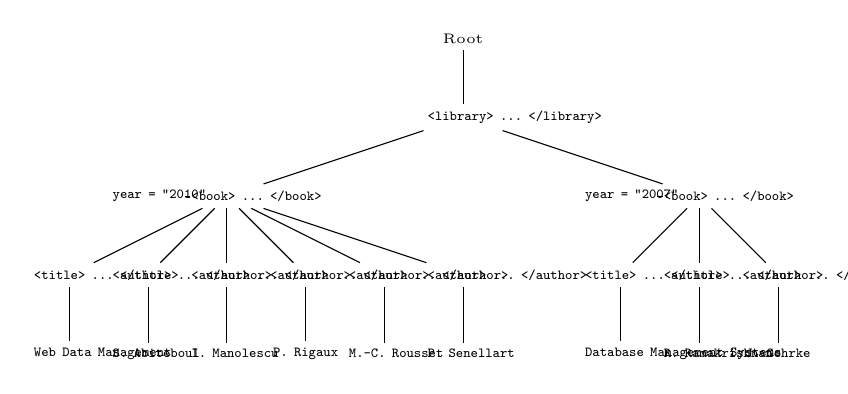
\begin{tikzpicture}[auto]
\tiny
  \tikzstyle{emptyStyle}=[text width=0.9cm, text centered]
  \tikzstyle{red}=[rounded corners=1mm,thick,draw=red!75,fill=red!20,text width=0.9cm, text centered]
  \tikzstyle{DarkViolet}=[rounded corners=1mm,thick,draw=DarkViolet!75,fill=DarkViolet!20,minimum size=7mm,text width=0.8cm, text centered]
  \tikzstyle{green}=[rounded corners=1mm,thick,draw=DarkOliveGreen!75,fill=DarkOliveGreen!20,minimum size=7mm,text width=0.8cm, text centered]
  \tikzstyle{cyan}=[rounded corners=1mm,thick,draw=DarkCyan!75,fill=DarkCyan!20,minimum size=7mm,text width=0.8cm, text centered]
 \tikzstyle{every label}=[black]
  \tikzstyle{HotPink}=[rounded corners=1mm,thick,draw=HotPink!75,fill=HotPink!20,minimum size=7mm,text width=0.8cm, text centered]
  \tikzstyle{Olive}=[rounded corners=1mm,thick,draw=Olive!75,fill=Olive!20,minimum size=7mm,text width=0.9cm, text centered]
  \tikzstyle{indiaRed}=[rounded corners=1mm,thick,draw=indiaRed!75,fill=indiaRed!20,minimum size=7mm,text width=0.9cm, text centered]

  \begin{scope}
    \node[emptyStyle](r) at (7,5) {Root};  
   %\node[emptyStyle](entete) at (3,4) {\texttt{$<?xml$ version $...>$}};
   %\draw[-] (r) -- (entete);
   \node[emptyStyle](library) at (7,4) {\verb?<library> ... </library>?};
   \draw[-] (r) -- (library);

    \node[emptyStyle](book1) at (4,3) {\verb?<book> ... </book>?};
   \draw[-] (library) -- (book1);
   \node[emptyStyle](book2) at (10,3) {\verb?<book> ... </book>?};
   \draw[-] (library) -- (book2);

    \node[emptyStyle](year1) at (3,3) {\verb?year = "2010"?};
   \draw[-] (book1) -- (year1);
    \node[emptyStyle](title1) at (2,2) {\verb?<title> ... </title>?};
   \draw[-] (book1) -- (title1);
 \node[emptyStyle](texttitle1) at (2,1) {\verb?Web Data Management?};
   \draw[-] (title1) -- (texttitle1);
    \node[emptyStyle](author1) at (3,2) {\verb?<author> ... </author>?};
   \draw[-] (book1) -- (author1);
   \node[emptyStyle](textauthor1) at (3,1) {\verb?S. Abiteboul?};
   \draw[-] (author1) -- (textauthor1);
    \node[emptyStyle](author2) at (4,2) {\verb?<author> ... </author>?};
   \draw[-] (book1) -- (author2);
   \node[emptyStyle](textauthor2) at (4,1) {\verb?I. Manolescu?};
   \draw[-] (author2) -- (textauthor2);
    \node[emptyStyle](author3) at (5,2) {\verb?<author> ... </author>?};
   \draw[-] (book1) -- (author3);
   \node[emptyStyle](textauthor3) at (5,1) {\verb?P. Rigaux?};
   \draw[-] (author3) -- (textauthor3);
    \node[emptyStyle](author4) at (6,2) {\verb?<author> ... </author>?};
   \draw[-] (book1) -- (author4);
   \node[emptyStyle](textauthor4) at (6,1) {\verb?M.-C. Rousset?};
   \draw[-] (author4) -- (textauthor4);
    \node[emptyStyle](author5) at (7,2) {\verb?<author> ... </author>?};
   \draw[-] (book1) -- (author5);
   \node[emptyStyle](textauthor5) at (7,1) {\verb?P. Senellart?};
   \draw[-] (author5) -- (textauthor5);

    \node[emptyStyle](year2) at (9,3) {\verb?year = "2007"?};
   \draw[-] (book2) -- (year2);
    \node[emptyStyle](title2) at (9,2) {\verb?<title> ... </title>?};
   \draw[-] (book2) -- (title2);
 \node[emptyStyle](texttitle2) at (9,1) {\verb?Database Management Systems?};
   \draw[-] (title2) -- (texttitle2);
    \node[emptyStyle](author1prime) at (10,2) {\verb?<author> ... </author>?};
   \draw[-] (book2) -- (author1prime);
   \node[emptyStyle](textauthor1prime) at (10,1) {\verb?R. Ramakrishnan?};
   \draw[-] (author1prime) -- (textauthor1prime);
    \node[emptyStyle](author2prime) at (11,2) {\verb?<author> ... </author>?};
   \draw[-] (book2) -- (author2prime);
   \node[emptyStyle](textauthor2prime) at (11,1) {\verb?J. Gehrke?};
   \draw[-] (author2prime) -- (textauthor2prime);

\end{scope}

\end{tikzpicture}

\begin{exoblock}  
\'Ecrire le fichier XML repr\'esent\'e ici sous forme d'arbre.
\prof{ce sera pour le following après}.
\end{exoblock}


\end{frame}

\begin{frame}{Quelques axes en exemple}

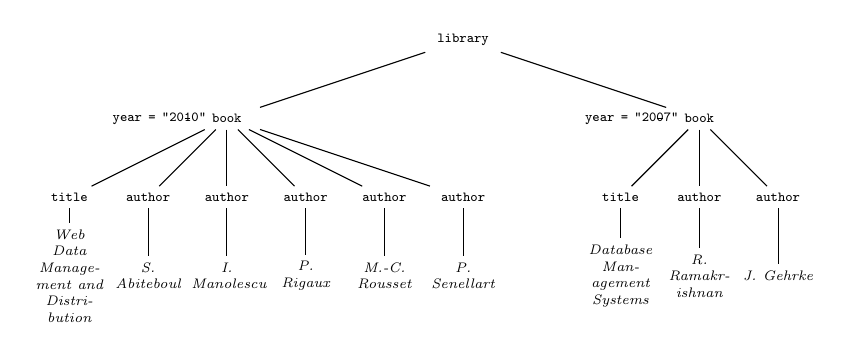
\begin{tikzpicture}[auto]
\tiny
  \tikzstyle{emptyStyle}=[text width=0.9cm, text centered]
  \tikzstyle{red}=[rounded corners=1mm,thick,draw=red!75,fill=red!20,text width=0.9cm, text centered]
  \tikzstyle{DarkViolet}=[rounded corners=1mm,thick,draw=DarkViolet!75,fill=DarkViolet!20,minimum size=7mm,text width=0.8cm, text centered]
  \tikzstyle{green}=[rounded corners=1mm,thick,draw=DarkOliveGreen!75,fill=DarkOliveGreen!20,minimum size=7mm,text width=0.8cm, text centered]
  \tikzstyle{cyan}=[rounded corners=1mm,thick,draw=DarkCyan!75,fill=DarkCyan!20,minimum size=7mm,text width=0.8cm, text centered]
 \tikzstyle{every label}=[black]
  \tikzstyle{HotPink}=[rounded corners=1mm,thick,draw=HotPink!75,fill=HotPink!20,minimum size=7mm,text width=0.8cm, text centered]
  \tikzstyle{Olive}=[rounded corners=1mm,thick,draw=Olive!75,fill=Olive!20,minimum size=7mm,text width=0.9cm, text centered]
  \tikzstyle{indiaRed}=[rounded corners=1mm,thick,draw=indiaRed!75,fill=indiaRed!20,minimum size=7mm,text width=0.9cm, text centered]

  \begin{scope}
   % \node[emptyStyle](r) at (7,5) {Root};  
   %\node[emptyStyle](entete) at (3,4) {\texttt{$<?xml$ version $...>$}};
   %\draw[-] (r) -- (entete);
   \node[emptyStyle](library) at (7,4) {\verb?library?};
   % \draw[-] (r) -- (library);

    \node[emptyStyle](book1) at (4,3) {\verb?book?};
   \draw[-] (library) -- (book1);
   \node[emptyStyle](book2) at (10,3) {\verb?book?};
   \draw[-] (library) -- (book2);

    \node[emptyStyle](year1) at (3,3) {\verb?year = "2010"?};
   \draw[-] (book1) -- (year1);
    \node[emptyStyle](title1) at (2,2) {\verb?title?};
   \draw[-] (book1) -- (title1);
 \node[emptyStyle](texttitle1) at (2,1) {\it Web Data Management and Distribution};
   \draw[-] (title1) -- (texttitle1);
    \node[emptyStyle](author1) at (3,2) {\verb?author?};
   \draw[-] (book1) -- (author1);
   \node[emptyStyle](textauthor1) at (3,1) {\it S. Abiteboul};
   \draw[-] (author1) -- (textauthor1);
    \node[emptyStyle](author2) at (4,2) {\verb?author?};
   \draw[-] (book1) -- (author2);
   \node[emptyStyle](textauthor2) at (4,1) {\it I. Manolescu};
   \draw[-] (author2) -- (textauthor2);
    \node[emptyStyle](author3) at (5,2) {\verb?author?};
   \draw[-] (book1) -- (author3);
   \node[emptyStyle](textauthor3) at (5,1) {\it P. Rigaux};
   \draw[-] (author3) -- (textauthor3);
    \node[emptyStyle](author4) at (6,2) {\verb?author?};
   \draw[-] (book1) -- (author4);
   \node[emptyStyle](textauthor4) at (6,1) {\it M.-C. Rousset};
   \draw[-] (author4) -- (textauthor4);
    \node[emptyStyle](author5) at (7,2) {\verb?author?};
   \draw[-] (book1) -- (author5);
   \node[emptyStyle](textauthor5) at (7,1) {\it P. Senellart};
   \draw[-] (author5) -- (textauthor5);

    \node[emptyStyle](year2) at (9,3) {\verb?year = "2007"?};
   \draw[-] (book2) -- (year2);
    \node[emptyStyle](title2) at (9,2) {\verb?title?};
   \draw[-] (book2) -- (title2);
 \node[emptyStyle](texttitle2) at (9,1) {\it Database Management Systems};
   \draw[-] (title2) -- (texttitle2);
    \node[emptyStyle](author1prime) at (10,2) {\verb?author?};
   \draw[-] (book2) -- (author1prime);
   \node[emptyStyle](textauthor1prime) at (10,1) {\it R. Ramakrishnan};
   \draw[-] (author1prime) -- (textauthor1prime);
    \node[emptyStyle](author2prime) at (11,2) {\verb?author?};
   \draw[-] (book2) -- (author2prime);
   \node[emptyStyle](textauthor2prime) at (11,1) {\it J. Gehrke};
   \draw[-] (author2prime) -- (textauthor2prime);

\end{scope}

\end{tikzpicture}


\end{frame}



\subsection{Child}

\begin{frame}{Quelques axes en exemple : Child}
\texttt{child} : Selects all children of the current node.

\bigskip

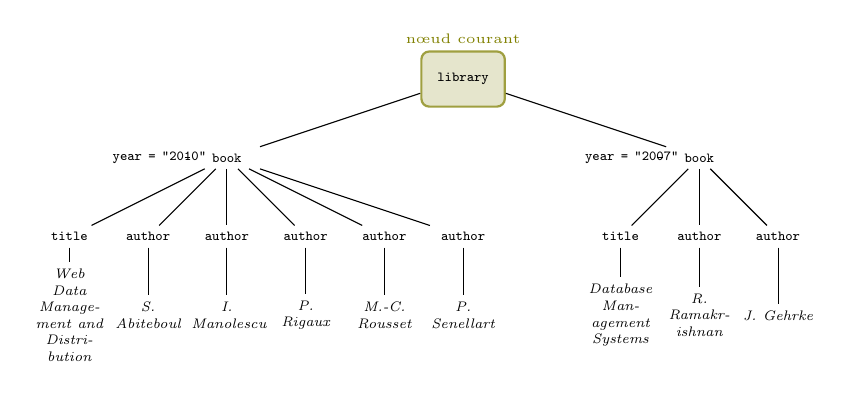
\begin{tikzpicture}[auto]
\tiny
  \tikzstyle{emptyStyle}=[text width=0.9cm, text centered]
  \tikzstyle{red}=[rounded corners=1mm,thick,draw=red!75,fill=red!20,text width=0.9cm, text centered]
  \tikzstyle{DarkViolet}=[rounded corners=1mm,thick,draw=DarkViolet!75,fill=DarkViolet!20,minimum size=7mm,text width=0.8cm, text centered]
  \tikzstyle{green}=[rounded corners=1mm,thick,draw=DarkOliveGreen!75,fill=DarkOliveGreen!20,minimum size=7mm,text width=0.8cm, text centered]
  \tikzstyle{cyan}=[rounded corners=1mm,thick,draw=DarkCyan!75,fill=DarkCyan!20,minimum size=7mm,text width=0.8cm, text centered]
 \tikzstyle{every label}=[black]
  \tikzstyle{HotPink}=[rounded corners=1mm,thick,draw=HotPink!75,fill=HotPink!20,minimum size=7mm,text width=0.8cm, text centered]
  \tikzstyle{noeudcourant}=[rounded corners=1mm,thick,draw=Olive!75,fill=Olive!20,minimum size=7mm,text width=0.9cm, text centered, label=\textcolor{Olive}{n{\oe}ud courant}]
  \tikzstyle{indiaRed}=[rounded corners=1mm,thick,draw=indiaRed!75,fill=indiaRed!20,minimum size=7mm,text width=0.9cm, text centered]

  \begin{scope}
   % \node[emptyStyle](r) at (7,5) {Root};  
   %\node[emptyStyle](entete) at (3,4) {\texttt{$<?xml$ version $...>$}};
   %\draw[-] (r) -- (entete);
   \node[noeudcourant](library) at (7,4) {\verb?library?};
   % \draw[-] (r) -- (library);

    \node[emptyStyle](book1) at (4,3) {\verb?book?};
   \draw[-] (library) -- (book1);
   \node[emptyStyle](book2) at (10,3) {\verb?book?};
   \draw[-] (library) -- (book2);

    \node[emptyStyle](year1) at (3,3) {\verb?year = "2010"?};
   \draw[-] (book1) -- (year1);
    \node[emptyStyle](title1) at (2,2) {\verb?title?};
   \draw[-] (book1) -- (title1);
 \node[emptyStyle](texttitle1) at (2,1) {\it Web Data Management and Distribution};
   \draw[-] (title1) -- (texttitle1);
    \node[emptyStyle](author1) at (3,2) {\verb?author?};
   \draw[-] (book1) -- (author1);
   \node[emptyStyle](textauthor1) at (3,1) {\it S. Abiteboul};
   \draw[-] (author1) -- (textauthor1);
    \node[emptyStyle](author2) at (4,2) {\verb?author?};
   \draw[-] (book1) -- (author2);
   \node[emptyStyle](textauthor2) at (4,1) {\it I. Manolescu};
   \draw[-] (author2) -- (textauthor2);
    \node[emptyStyle](author3) at (5,2) {\verb?author?};
   \draw[-] (book1) -- (author3);
   \node[emptyStyle](textauthor3) at (5,1) {\it P. Rigaux};
   \draw[-] (author3) -- (textauthor3);
    \node[emptyStyle](author4) at (6,2) {\verb?author?};
   \draw[-] (book1) -- (author4);
   \node[emptyStyle](textauthor4) at (6,1) {\it M.-C. Rousset};
   \draw[-] (author4) -- (textauthor4);
    \node[emptyStyle](author5) at (7,2) {\verb?author?};
   \draw[-] (book1) -- (author5);
   \node[emptyStyle](textauthor5) at (7,1) {\it P. Senellart};
   \draw[-] (author5) -- (textauthor5);

    \node[emptyStyle](year2) at (9,3) {\verb?year = "2007"?};
   \draw[-] (book2) -- (year2);
    \node[emptyStyle](title2) at (9,2) {\verb?title?};
   \draw[-] (book2) -- (title2);
 \node[emptyStyle](texttitle2) at (9,1) {\it Database Management Systems};
   \draw[-] (title2) -- (texttitle2);
    \node[emptyStyle](author1prime) at (10,2) {\verb?author?};
   \draw[-] (book2) -- (author1prime);
   \node[emptyStyle](textauthor1prime) at (10,1) {\it R. Ramakrishnan};
   \draw[-] (author1prime) -- (textauthor1prime);
    \node[emptyStyle](author2prime) at (11,2) {\verb?author?};
   \draw[-] (book2) -- (author2prime);
   \node[emptyStyle](textauthor2prime) at (11,1) {\it J. Gehrke};
   \draw[-] (author2prime) -- (textauthor2prime);
\end{scope}
\end{tikzpicture}
\end{frame}


\begin{frame}{Quelques axes en exemple : Child}
\texttt{child} : Selects all children of the current node.

\bigskip

\begin{tikzpicture}[auto]
\tiny
  \tikzstyle{emptyStyle}=[text width=0.9cm, text centered]
  \tikzstyle{red}=[rounded corners=1mm,thick,draw=red!75,fill=red!20,text width=0.9cm, text centered]
  \tikzstyle{DarkViolet}=[rounded corners=1mm,thick,draw=DarkViolet!75,fill=DarkViolet!20,minimum size=7mm,text width=0.8cm, text centered]
  \tikzstyle{green}=[rounded corners=1mm,thick,draw=DarkOliveGreen!75,fill=DarkOliveGreen!20,minimum size=7mm,text width=0.8cm, text centered]
  \tikzstyle{cyan}=[rounded corners=1mm,thick,draw=DarkCyan!75,fill=DarkCyan!20,minimum size=7mm,text width=0.8cm, text centered]
 \tikzstyle{every label}=[black]
  \tikzstyle{HotPink}=[rounded corners=1mm,thick,draw=HotPink!75,fill=HotPink!20,minimum size=7mm,text width=0.8cm, text centered]
  \tikzstyle{noeudcourant}=[rounded corners=1mm,thick,draw=Olive!75,fill=Olive!20,minimum size=7mm,text width=0.9cm, text centered, label=\textcolor{Olive}{n{\oe}ud courant}]
  \tikzstyle{indiaRed}=[rounded corners=1mm,thick,draw=indiaRed!75,fill=indiaRed!20,minimum size=7mm,text width=0.9cm, text centered]

  \begin{scope}
   % \node[emptyStyle](r) at (7,5) {Root};  
   %\node[emptyStyle](entete) at (3,4) {\texttt{$<?xml$ version $...>$}};
   %\draw[-] (r) -- (entete);
   \node[noeudcourant](library) at (7,4) {\verb?library?};
   %\draw[-] (r) -- (library);

    \node[indiaRed](book1) at (4,3) {\verb?book?};
   \draw[-] (library) -- (book1);
   \node[indiaRed](book2) at (10,3) {\verb?book?};
   \draw[-] (library) -- (book2);

    \node[emptyStyle](year1) at (3,3) {\verb?year = "2010"?};
   \draw[-] (book1) -- (year1);
    \node[emptyStyle](title1) at (2,2) {\verb?title?};
   \draw[-] (book1) -- (title1);
 \node[emptyStyle](texttitle1) at (2,1) {\it Web Data Management and Distribution};
   \draw[-] (title1) -- (texttitle1);
    \node[emptyStyle](author1) at (3,2) {\verb?author?};
   \draw[-] (book1) -- (author1);
   \node[emptyStyle](textauthor1) at (3,1) {\it S. Abiteboul};
   \draw[-] (author1) -- (textauthor1);
    \node[emptyStyle](author2) at (4,2) {\verb?author?};
   \draw[-] (book1) -- (author2);
   \node[emptyStyle](textauthor2) at (4,1) {\it I. Manolescu};
   \draw[-] (author2) -- (textauthor2);
    \node[emptyStyle](author3) at (5,2) {\verb?author?};
   \draw[-] (book1) -- (author3);
   \node[emptyStyle](textauthor3) at (5,1) {\it P. Rigaux};
   \draw[-] (author3) -- (textauthor3);
    \node[emptyStyle](author4) at (6,2) {\verb?author?};
   \draw[-] (book1) -- (author4);
   \node[emptyStyle](textauthor4) at (6,1) {\it M.-C. Rousset};
   \draw[-] (author4) -- (textauthor4);
    \node[emptyStyle](author5) at (7,2) {\verb?author?};
   \draw[-] (book1) -- (author5);
   \node[emptyStyle](textauthor5) at (7,1) {\it P. Senellart};
   \draw[-] (author5) -- (textauthor5);

    \node[emptyStyle](year2) at (9,3) {\verb?year = "2007"?};
   \draw[-] (book2) -- (year2);
    \node[emptyStyle](title2) at (9,2) {\verb?title?};
   \draw[-] (book2) -- (title2);
 \node[emptyStyle](texttitle2) at (9,1) {\it Database Management Systems};
   \draw[-] (title2) -- (texttitle2);
    \node[emptyStyle](author1prime) at (10,2) {\verb?author?};
   \draw[-] (book2) -- (author1prime);
   \node[emptyStyle](textauthor1prime) at (10,1) {\it R. Ramakrishnan};
   \draw[-] (author1prime) -- (textauthor1prime);
    \node[emptyStyle](author2prime) at (11,2) {\verb?author?};
   \draw[-] (book2) -- (author2prime);
   \node[emptyStyle](textauthor2prime) at (11,1) {\it J. Gehrke};
   \draw[-] (author2prime) -- (textauthor2prime);
\end{scope}
\end{tikzpicture}
\end{frame} 

\begin{frame}{Quelques axes en exemple : Child}
\texttt{child} : Selects all children of the current node.

\bigskip

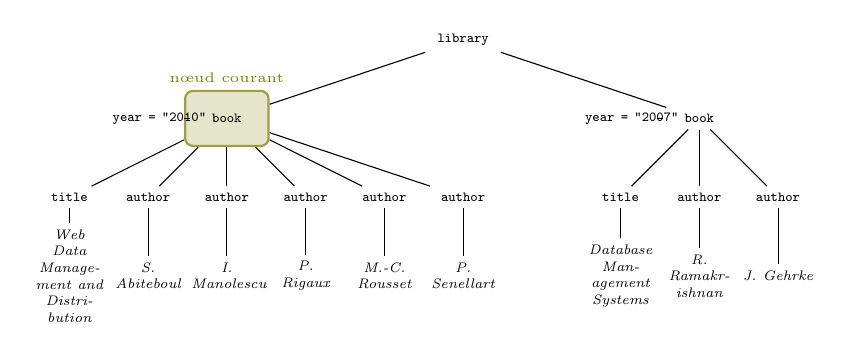
\begin{tikzpicture}[auto]
\tiny
  \tikzstyle{emptyStyle}=[text width=0.9cm, text centered]
  \tikzstyle{red}=[rounded corners=1mm,thick,draw=red!75,fill=red!20,text width=0.9cm, text centered]
  \tikzstyle{DarkViolet}=[rounded corners=1mm,thick,draw=DarkViolet!75,fill=DarkViolet!20,minimum size=7mm,text width=0.8cm, text centered]
  \tikzstyle{green}=[rounded corners=1mm,thick,draw=DarkOliveGreen!75,fill=DarkOliveGreen!20,minimum size=7mm,text width=0.8cm, text centered]
  \tikzstyle{cyan}=[rounded corners=1mm,thick,draw=DarkCyan!75,fill=DarkCyan!20,minimum size=7mm,text width=0.8cm, text centered]
 \tikzstyle{every label}=[black]
  \tikzstyle{HotPink}=[rounded corners=1mm,thick,draw=HotPink!75,fill=HotPink!20,minimum size=7mm,text width=0.8cm, text centered]
  \tikzstyle{noeudcourant}=[rounded corners=1mm,thick,draw=Olive!75,fill=Olive!20,minimum size=7mm,text width=0.9cm, text centered, label=\textcolor{Olive}{n{\oe}ud courant}]
  \tikzstyle{indiaRed}=[rounded corners=1mm,thick,draw=indiaRed!75,fill=indiaRed!20,minimum size=7mm,text width=0.9cm, text centered]

  \begin{scope}
   % \node[emptyStyle](r) at (7,5) {Root};  
   %\node[emptyStyle](entete) at (3,4) {\texttt{$<?xml$ version $...>$}};
   %\draw[-] (r) -- (entete);
   \node[emptyStyle](library) at (7,4) {\verb?library?};
   % \draw[-] (r) -- (library);

    \node[noeudcourant](book1) at (4,3) {\verb?book?};
   \draw[-] (library) -- (book1);
   \node[emptyStyle](book2) at (10,3) {\verb?book?};
   \draw[-] (library) -- (book2);

    \node[emptyStyle](year1) at (3,3) {\verb?year = "2010"?};
   \draw[-] (book1) -- (year1);
    \node[emptyStyle](title1) at (2,2) {\verb?title?};
   \draw[-] (book1) -- (title1);
 \node[emptyStyle](texttitle1) at (2,1) {\it Web Data Management and Distribution};
   \draw[-] (title1) -- (texttitle1);
    \node[emptyStyle](author1) at (3,2) {\verb?author?};
   \draw[-] (book1) -- (author1);
   \node[emptyStyle](textauthor1) at (3,1) {\it S. Abiteboul};
   \draw[-] (author1) -- (textauthor1);
    \node[emptyStyle](author2) at (4,2) {\verb?author?};
   \draw[-] (book1) -- (author2);
   \node[emptyStyle](textauthor2) at (4,1) {\it I. Manolescu};
   \draw[-] (author2) -- (textauthor2);
    \node[emptyStyle](author3) at (5,2) {\verb?author?};
   \draw[-] (book1) -- (author3);
   \node[emptyStyle](textauthor3) at (5,1) {\it P. Rigaux};
   \draw[-] (author3) -- (textauthor3);
    \node[emptyStyle](author4) at (6,2) {\verb?author?};
   \draw[-] (book1) -- (author4);
   \node[emptyStyle](textauthor4) at (6,1) {\it M.-C. Rousset};
   \draw[-] (author4) -- (textauthor4);
    \node[emptyStyle](author5) at (7,2) {\verb?author?};
   \draw[-] (book1) -- (author5);
   \node[emptyStyle](textauthor5) at (7,1) {\it P. Senellart};
   \draw[-] (author5) -- (textauthor5);

    \node[emptyStyle](year2) at (9,3) {\verb?year = "2007"?};
   \draw[-] (book2) -- (year2);
    \node[emptyStyle](title2) at (9,2) {\verb?title?};
   \draw[-] (book2) -- (title2);
 \node[emptyStyle](texttitle2) at (9,1) {\it Database Management Systems};
   \draw[-] (title2) -- (texttitle2);
    \node[emptyStyle](author1prime) at (10,2) {\verb?author?};
   \draw[-] (book2) -- (author1prime);
   \node[emptyStyle](textauthor1prime) at (10,1) {\it R. Ramakrishnan};
   \draw[-] (author1prime) -- (textauthor1prime);
    \node[emptyStyle](author2prime) at (11,2) {\verb?author?};
   \draw[-] (book2) -- (author2prime);
   \node[emptyStyle](textauthor2prime) at (11,1) {\it J. Gehrke};
   \draw[-] (author2prime) -- (textauthor2prime);
\end{scope}
\end{tikzpicture}
\end{frame}


\begin{frame}{Quelques axes en exemple : Child}
\texttt{child} : Selects all children of the current node.

\bigskip

\begin{tikzpicture}[auto]
\tiny
  \tikzstyle{emptyStyle}=[text width=0.9cm, text centered]
  \tikzstyle{red}=[rounded corners=1mm,thick,draw=red!75,fill=red!20,text width=0.9cm, text centered]
  \tikzstyle{DarkViolet}=[rounded corners=1mm,thick,draw=DarkViolet!75,fill=DarkViolet!20,minimum size=7mm,text width=0.8cm, text centered]
  \tikzstyle{green}=[rounded corners=1mm,thick,draw=DarkOliveGreen!75,fill=DarkOliveGreen!20,minimum size=7mm,text width=0.8cm, text centered]
  \tikzstyle{cyan}=[rounded corners=1mm,thick,draw=DarkCyan!75,fill=DarkCyan!20,minimum size=7mm,text width=0.8cm, text centered]
 \tikzstyle{every label}=[black]
  \tikzstyle{HotPink}=[rounded corners=1mm,thick,draw=HotPink!75,fill=HotPink!20,minimum size=7mm,text width=0.8cm, text centered]
  \tikzstyle{noeudcourant}=[rounded corners=1mm,thick,draw=Olive!75,fill=Olive!20,minimum size=7mm,text width=0.9cm, text centered, label=\textcolor{Olive}{n{\oe}ud courant}]
  \tikzstyle{indiaRed}=[rounded corners=1mm,thick,draw=indiaRed!75,fill=indiaRed!20,minimum size=7mm,text width=0.9cm, text centered]

  \begin{scope}
   % \node[emptyStyle](r) at (7,5) {Root};  
   %\node[emptyStyle](entete) at (3,4) {\texttt{$<?xml$ version $...>$}};
   %\draw[-] (r) -- (entete);
   \node[emptyStyle](library) at (7,4) {\verb?library?};
   % \draw[-] (r) -- (library);

    \node[noeudcourant](book1) at (4,3) {\verb?book?};
   \draw[-] (library) -- (book1);
   \node[emptyStyle](book2) at (10,3) {\verb?book?};
   \draw[-] (library) -- (book2);

    \node[emptyStyle](year1) at (3,3) {\verb?year = "2010"?};
   \draw[-] (book1) -- (year1);
    \node[indiaRed](title1) at (2,2) {\verb?title?};
   \draw[-] (book1) -- (title1);
 \node[emptyStyle](texttitle1) at (2,1) {\it Web Data Management and Distribution};
   \draw[-] (title1) -- (texttitle1);
    \node[indiaRed](author1) at (3,2) {\verb?author?};
   \draw[-] (book1) -- (author1);
   \node[emptyStyle](textauthor1) at (3,1) {\it S. Abiteboul};
   \draw[-] (author1) -- (textauthor1);
    \node[indiaRed](author2) at (4,2) {\verb?author?};
   \draw[-] (book1) -- (author2);
   \node[emptyStyle](textauthor2) at (4,1) {\it I. Manolescu};
   \draw[-] (author2) -- (textauthor2);
    \node[indiaRed](author3) at (5,2) {\verb?author?};
   \draw[-] (book1) -- (author3);
   \node[emptyStyle](textauthor3) at (5,1) {\it P. Rigaux};
   \draw[-] (author3) -- (textauthor3);
    \node[indiaRed](author4) at (6,2) {\verb?author?};
   \draw[-] (book1) -- (author4);
   \node[emptyStyle](textauthor4) at (6,1) {\it M.-C. Rousset};
   \draw[-] (author4) -- (textauthor4);
    \node[indiaRed](author5) at (7,2) {\verb?author?};
   \draw[-] (book1) -- (author5);
   \node[emptyStyle](textauthor5) at (7,1) {\it P. Senellart};
   \draw[-] (author5) -- (textauthor5);

    \node[emptyStyle](year2) at (9,3) {\verb?year = "2007"?};
   \draw[-] (book2) -- (year2);
    \node[emptyStyle](title2) at (9,2) {\verb?title?};
   \draw[-] (book2) -- (title2);
 \node[emptyStyle](texttitle2) at (9,1) {\it Database Management Systems};
   \draw[-] (title2) -- (texttitle2);
    \node[emptyStyle](author1prime) at (10,2) {\verb?author?};
   \draw[-] (book2) -- (author1prime);
   \node[emptyStyle](textauthor1prime) at (10,1) {\it R. Ramakrishnan};
   \draw[-] (author1prime) -- (textauthor1prime);
    \node[emptyStyle](author2prime) at (11,2) {\verb?author?};
   \draw[-] (book2) -- (author2prime);
   \node[emptyStyle](textauthor2prime) at (11,1) {\it J. Gehrke};
   \draw[-] (author2prime) -- (textauthor2prime);
\end{scope}
\end{tikzpicture}
\end{frame}


\subsection{Parent}

% Parent

\begin{frame}{Quelques axes en exemple : Parent}
\texttt{parent} : Selects the parent of the current node.

\bigskip

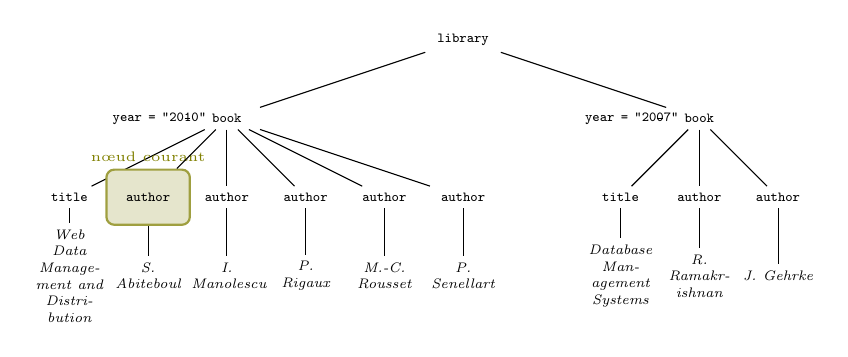
\begin{tikzpicture}[auto]
\tiny
  \tikzstyle{emptyStyle}=[text width=0.9cm, text centered]
  \tikzstyle{red}=[rounded corners=1mm,thick,draw=red!75,fill=red!20,text width=0.9cm, text centered]
  \tikzstyle{DarkViolet}=[rounded corners=1mm,thick,draw=DarkViolet!75,fill=DarkViolet!20,minimum size=7mm,text width=0.8cm, text centered]
  \tikzstyle{green}=[rounded corners=1mm,thick,draw=DarkOliveGreen!75,fill=DarkOliveGreen!20,minimum size=7mm,text width=0.8cm, text centered]
  \tikzstyle{cyan}=[rounded corners=1mm,thick,draw=DarkCyan!75,fill=DarkCyan!20,minimum size=7mm,text width=0.8cm, text centered]
 \tikzstyle{every label}=[black]
  \tikzstyle{HotPink}=[rounded corners=1mm,thick,draw=HotPink!75,fill=HotPink!20,minimum size=7mm,text width=0.8cm, text centered]
  \tikzstyle{noeudcourant}=[rounded corners=1mm,thick,draw=Olive!75,fill=Olive!20,minimum size=7mm,text width=0.9cm, text centered, label=\textcolor{Olive}{n{\oe}ud courant}]
  \tikzstyle{indiaRed}=[rounded corners=1mm,thick,draw=indiaRed!75,fill=indiaRed!20,minimum size=7mm,text width=0.9cm, text centered]

  \begin{scope}
   % \node[emptyStyle](r) at (7,5) {Root};  
   %\node[emptyStyle](entete) at (3,4) {\texttt{$<?xml$ version $...>$}};
   %\draw[-] (r) -- (entete);
   \node[emptyStyle](library) at (7,4) {\verb?library?};
   % \draw[-] (r) -- (library);

    \node[emptyStyle](book1) at (4,3) {\verb?book?};
   \draw[-] (library) -- (book1);
   \node[emptyStyle](book2) at (10,3) {\verb?book?};
   \draw[-] (library) -- (book2);

    \node[emptyStyle](year1) at (3,3) {\verb?year = "2010"?};
   \draw[-] (book1) -- (year1);
    \node[emptyStyle](title1) at (2,2) {\verb?title?};
   \draw[-] (book1) -- (title1);
 \node[emptyStyle](texttitle1) at (2,1) {\it Web Data Management and Distribution};
   \draw[-] (title1) -- (texttitle1);
    \node[noeudcourant](author1) at (3,2) {\verb?author?};
   \draw[-] (book1) -- (author1);
   \node[emptyStyle](textauthor1) at (3,1) {\it S. Abiteboul};
   \draw[-] (author1) -- (textauthor1);
    \node[emptyStyle](author2) at (4,2) {\verb?author?};
   \draw[-] (book1) -- (author2);
   \node[emptyStyle](textauthor2) at (4,1) {\it I. Manolescu};
   \draw[-] (author2) -- (textauthor2);
    \node[emptyStyle](author3) at (5,2) {\verb?author?};
   \draw[-] (book1) -- (author3);
   \node[emptyStyle](textauthor3) at (5,1) {\it P. Rigaux};
   \draw[-] (author3) -- (textauthor3);
    \node[emptyStyle](author4) at (6,2) {\verb?author?};
   \draw[-] (book1) -- (author4);
   \node[emptyStyle](textauthor4) at (6,1) {\it M.-C. Rousset};
   \draw[-] (author4) -- (textauthor4);
    \node[emptyStyle](author5) at (7,2) {\verb?author?};
   \draw[-] (book1) -- (author5);
   \node[emptyStyle](textauthor5) at (7,1) {\it P. Senellart};
   \draw[-] (author5) -- (textauthor5);

    \node[emptyStyle](year2) at (9,3) {\verb?year = "2007"?};
   \draw[-] (book2) -- (year2);
    \node[emptyStyle](title2) at (9,2) {\verb?title?};
   \draw[-] (book2) -- (title2);
 \node[emptyStyle](texttitle2) at (9,1) {\it Database Management Systems};
   \draw[-] (title2) -- (texttitle2);
    \node[emptyStyle](author1prime) at (10,2) {\verb?author?};
   \draw[-] (book2) -- (author1prime);
   \node[emptyStyle](textauthor1prime) at (10,1) {\it R. Ramakrishnan};
   \draw[-] (author1prime) -- (textauthor1prime);
    \node[emptyStyle](author2prime) at (11,2) {\verb?author?};
   \draw[-] (book2) -- (author2prime);
   \node[emptyStyle](textauthor2prime) at (11,1) {\it J. Gehrke};
   \draw[-] (author2prime) -- (textauthor2prime);
\end{scope}
\end{tikzpicture}
\end{frame}


\begin{frame}{Quelques axes en exemple : Parent}
\texttt{parent} : Selects the parent of the current node.

\bigskip

\begin{tikzpicture}[auto]
\tiny
  \tikzstyle{emptyStyle}=[text width=0.9cm, text centered]
  \tikzstyle{red}=[rounded corners=1mm,thick,draw=red!75,fill=red!20,text width=0.9cm, text centered]
  \tikzstyle{DarkViolet}=[rounded corners=1mm,thick,draw=DarkViolet!75,fill=DarkViolet!20,minimum size=7mm,text width=0.8cm, text centered]
  \tikzstyle{green}=[rounded corners=1mm,thick,draw=DarkOliveGreen!75,fill=DarkOliveGreen!20,minimum size=7mm,text width=0.8cm, text centered]
  \tikzstyle{cyan}=[rounded corners=1mm,thick,draw=DarkCyan!75,fill=DarkCyan!20,minimum size=7mm,text width=0.8cm, text centered]
 \tikzstyle{every label}=[black]
  \tikzstyle{HotPink}=[rounded corners=1mm,thick,draw=HotPink!75,fill=HotPink!20,minimum size=7mm,text width=0.8cm, text centered]
  \tikzstyle{noeudcourant}=[rounded corners=1mm,thick,draw=Olive!75,fill=Olive!20,minimum size=7mm,text width=0.9cm, text centered, label=\textcolor{Olive}{n{\oe}ud courant}]
  \tikzstyle{indiaRed}=[rounded corners=1mm,thick,draw=indiaRed!75,fill=indiaRed!20,minimum size=7mm,text width=0.9cm, text centered]

  \begin{scope}
   % \node[emptyStyle](r) at (7,5) {Root};  
   %\node[emptyStyle](entete) at (3,4) {\texttt{$<?xml$ version $...>$}};
   %\draw[-] (r) -- (entete);
   \node[emptyStyle](library) at (7,4) {\verb?library?};
   % \draw[-] (r) -- (library);

    \node[indiaRed](book1) at (4,3) {\verb?book?};
   \draw[-] (library) -- (book1);
   \node[emptyStyle](book2) at (10,3) {\verb?book?};
   \draw[-] (library) -- (book2);

    \node[emptyStyle](year1) at (3,3) {\verb?year = "2010"?};
   \draw[-] (book1) -- (year1);
    \node[emptyStyle](title1) at (2,2) {\verb?title?};
   \draw[-] (book1) -- (title1);
 \node[emptyStyle](texttitle1) at (2,1) {\it Web Data Management and Distribution};
   \draw[-] (title1) -- (texttitle1);
    \node[noeudcourant](author1) at (3,2) {\verb?author?};
   \draw[-] (book1) -- (author1);
   \node[emptyStyle](textauthor1) at (3,1) {\it S. Abiteboul};
   \draw[-] (author1) -- (textauthor1);
    \node[emptyStyle](author2) at (4,2) {\verb?author?};
   \draw[-] (book1) -- (author2);
   \node[emptyStyle](textauthor2) at (4,1) {\it I. Manolescu};
   \draw[-] (author2) -- (textauthor2);
    \node[emptyStyle](author3) at (5,2) {\verb?author?};
   \draw[-] (book1) -- (author3);
   \node[emptyStyle](textauthor3) at (5,1) {\it P. Rigaux};
   \draw[-] (author3) -- (textauthor3);
    \node[emptyStyle](author4) at (6,2) {\verb?author?};
   \draw[-] (book1) -- (author4);
   \node[emptyStyle](textauthor4) at (6,1) {\it M.-C. Rousset};
   \draw[-] (author4) -- (textauthor4);
    \node[emptyStyle](author5) at (7,2) {\verb?author?};
   \draw[-] (book1) -- (author5);
   \node[emptyStyle](textauthor5) at (7,1) {\it P. Senellart};
   \draw[-] (author5) -- (textauthor5);

    \node[emptyStyle](year2) at (9,3) {\verb?year = "2007"?};
   \draw[-] (book2) -- (year2);
    \node[emptyStyle](title2) at (9,2) {\verb?title?};
   \draw[-] (book2) -- (title2);
 \node[emptyStyle](texttitle2) at (9,1) {\it Database Management Systems};
   \draw[-] (title2) -- (texttitle2);
    \node[emptyStyle](author1prime) at (10,2) {\verb?author?};
   \draw[-] (book2) -- (author1prime);
   \node[emptyStyle](textauthor1prime) at (10,1) {\it R. Ramakrishnan};
   \draw[-] (author1prime) -- (textauthor1prime);
    \node[emptyStyle](author2prime) at (11,2) {\verb?author?};
   \draw[-] (book2) -- (author2prime);
   \node[emptyStyle](textauthor2prime) at (11,1) {\it J. Gehrke};
   \draw[-] (author2prime) -- (textauthor2prime);
\end{scope}
\end{tikzpicture}
\end{frame}

\begin{frame}{Quelques axes en exemple : Parent}
\texttt{parent} : Selects the parent of the current node.

\bigskip

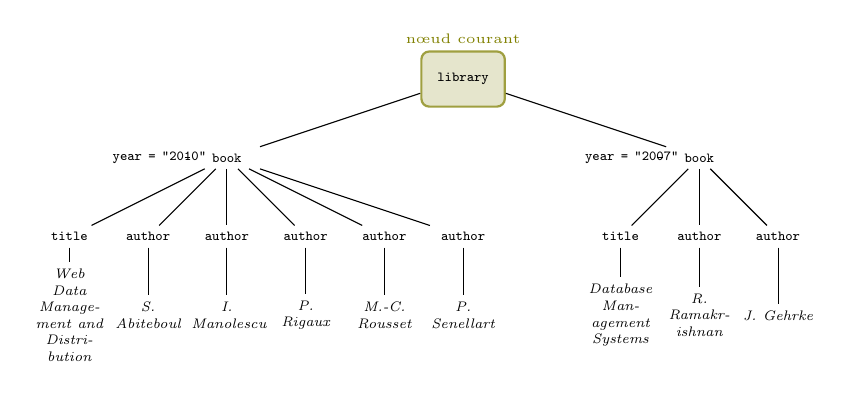
\begin{tikzpicture}[auto]
\tiny
  \tikzstyle{emptyStyle}=[text width=0.9cm, text centered]
  \tikzstyle{red}=[rounded corners=1mm,thick,draw=red!75,fill=red!20,text width=0.9cm, text centered]
  \tikzstyle{DarkViolet}=[rounded corners=1mm,thick,draw=DarkViolet!75,fill=DarkViolet!20,minimum size=7mm,text width=0.8cm, text centered]
  \tikzstyle{green}=[rounded corners=1mm,thick,draw=DarkOliveGreen!75,fill=DarkOliveGreen!20,minimum size=7mm,text width=0.8cm, text centered]
  \tikzstyle{cyan}=[rounded corners=1mm,thick,draw=DarkCyan!75,fill=DarkCyan!20,minimum size=7mm,text width=0.8cm, text centered]
 \tikzstyle{every label}=[black]
  \tikzstyle{HotPink}=[rounded corners=1mm,thick,draw=HotPink!75,fill=HotPink!20,minimum size=7mm,text width=0.8cm, text centered]
  \tikzstyle{noeudcourant}=[rounded corners=1mm,thick,draw=Olive!75,fill=Olive!20,minimum size=7mm,text width=0.9cm, text centered, label=\textcolor{Olive}{n{\oe}ud courant}]
  \tikzstyle{indiaRed}=[rounded corners=1mm,thick,draw=indiaRed!75,fill=indiaRed!20,minimum size=7mm,text width=0.9cm, text centered]

  \begin{scope}
   % \node[emptyStyle](r) at (7,5) {Root};  
   %\node[emptyStyle](entete) at (3,4) {\texttt{$<?xml$ version $...>$}};
   %\draw[-] (r) -- (entete);
   \node[noeudcourant](library) at (7,4) {\verb?library?};
   % \draw[-] (r) -- (library);

    \node[emptyStyle](book1) at (4,3) {\verb?book?};
   \draw[-] (library) -- (book1);
   \node[emptyStyle](book2) at (10,3) {\verb?book?};
   \draw[-] (library) -- (book2);

    \node[emptyStyle](year1) at (3,3) {\verb?year = "2010"?};
   \draw[-] (book1) -- (year1);
    \node[emptyStyle](title1) at (2,2) {\verb?title?};
   \draw[-] (book1) -- (title1);
 \node[emptyStyle](texttitle1) at (2,1) {\it Web Data Management and Distribution};
   \draw[-] (title1) -- (texttitle1);
    \node[emptyStyle](author1) at (3,2) {\verb?author?};
   \draw[-] (book1) -- (author1);
   \node[emptyStyle](textauthor1) at (3,1) {\it S. Abiteboul};
   \draw[-] (author1) -- (textauthor1);
    \node[emptyStyle](author2) at (4,2) {\verb?author?};
   \draw[-] (book1) -- (author2);
   \node[emptyStyle](textauthor2) at (4,1) {\it I. Manolescu};
   \draw[-] (author2) -- (textauthor2);
    \node[emptyStyle](author3) at (5,2) {\verb?author?};
   \draw[-] (book1) -- (author3);
   \node[emptyStyle](textauthor3) at (5,1) {\it P. Rigaux};
   \draw[-] (author3) -- (textauthor3);
    \node[emptyStyle](author4) at (6,2) {\verb?author?};
   \draw[-] (book1) -- (author4);
   \node[emptyStyle](textauthor4) at (6,1) {\it M.-C. Rousset};
   \draw[-] (author4) -- (textauthor4);
    \node[emptyStyle](author5) at (7,2) {\verb?author?};
   \draw[-] (book1) -- (author5);
   \node[emptyStyle](textauthor5) at (7,1) {\it P. Senellart};
   \draw[-] (author5) -- (textauthor5);

    \node[emptyStyle](year2) at (9,3) {\verb?year = "2007"?};
   \draw[-] (book2) -- (year2);
    \node[emptyStyle](title2) at (9,2) {\verb?title?};
   \draw[-] (book2) -- (title2);
 \node[emptyStyle](texttitle2) at (9,1) {\it Database Management Systems};
   \draw[-] (title2) -- (texttitle2);
    \node[emptyStyle](author1prime) at (10,2) {\verb?author?};
   \draw[-] (book2) -- (author1prime);
   \node[emptyStyle](textauthor1prime) at (10,1) {\it R. Ramakrishnan};
   \draw[-] (author1prime) -- (textauthor1prime);
    \node[emptyStyle](author2prime) at (11,2) {\verb?author?};
   \draw[-] (book2) -- (author2prime);
   \node[emptyStyle](textauthor2prime) at (11,1) {\it J. Gehrke};
   \draw[-] (author2prime) -- (textauthor2prime);
\end{scope}
\end{tikzpicture}
\prof{Pas de n{\oe}ud parent}

\end{frame}


% ancestor
\subsection{Ancestor}

\begin{frame}{Quelques axes en exemple : Ancestor}
\texttt{ancestor} : Selects all ancestors (parent, grandparent, etc.) of the current node

\bigskip

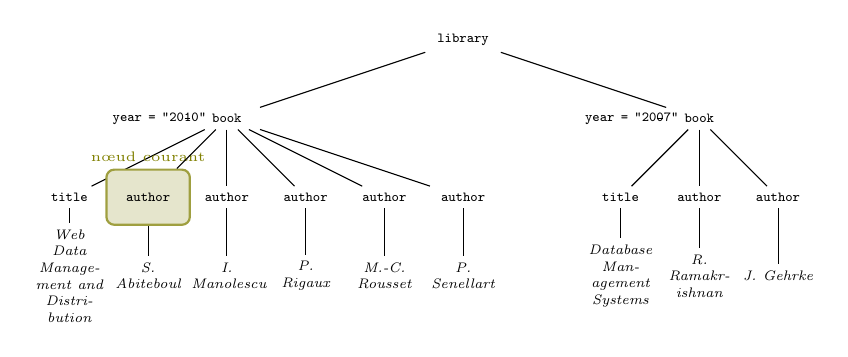
\begin{tikzpicture}[auto]
\tiny
  \tikzstyle{emptyStyle}=[text width=0.9cm, text centered]
  \tikzstyle{red}=[rounded corners=1mm,thick,draw=red!75,fill=red!20,text width=0.9cm, text centered]
  \tikzstyle{DarkViolet}=[rounded corners=1mm,thick,draw=DarkViolet!75,fill=DarkViolet!20,minimum size=7mm,text width=0.8cm, text centered]
  \tikzstyle{green}=[rounded corners=1mm,thick,draw=DarkOliveGreen!75,fill=DarkOliveGreen!20,minimum size=7mm,text width=0.8cm, text centered]
  \tikzstyle{cyan}=[rounded corners=1mm,thick,draw=DarkCyan!75,fill=DarkCyan!20,minimum size=7mm,text width=0.8cm, text centered]
 \tikzstyle{every label}=[black]
  \tikzstyle{HotPink}=[rounded corners=1mm,thick,draw=HotPink!75,fill=HotPink!20,minimum size=7mm,text width=0.8cm, text centered]
  \tikzstyle{noeudcourant}=[rounded corners=1mm,thick,draw=Olive!75,fill=Olive!20,minimum size=7mm,text width=0.9cm, text centered, label=\textcolor{Olive}{n{\oe}ud courant}]
  \tikzstyle{indiaRed}=[rounded corners=1mm,thick,draw=indiaRed!75,fill=indiaRed!20,minimum size=7mm,text width=0.9cm, text centered]

  \begin{scope}
   % \node[emptyStyle](r) at (7,5) {Root};  
   %\node[emptyStyle](entete) at (3,4) {\texttt{$<?xml$ version $...>$}};
   %\draw[-] (r) -- (entete);
   \node[emptyStyle](library) at (7,4) {\verb?library?};
   % \draw[-] (r) -- (library);

    \node[emptyStyle](book1) at (4,3) {\verb?book?};
   \draw[-] (library) -- (book1);
   \node[emptyStyle](book2) at (10,3) {\verb?book?};
   \draw[-] (library) -- (book2);

    \node[emptyStyle](year1) at (3,3) {\verb?year = "2010"?};
   \draw[-] (book1) -- (year1);
    \node[emptyStyle](title1) at (2,2) {\verb?title?};
   \draw[-] (book1) -- (title1);
 \node[emptyStyle](texttitle1) at (2,1) {\it Web Data Management and Distribution};
   \draw[-] (title1) -- (texttitle1);
    \node[noeudcourant](author1) at (3,2) {\verb?author?};
   \draw[-] (book1) -- (author1);
   \node[emptyStyle](textauthor1) at (3,1) {\it S. Abiteboul};
   \draw[-] (author1) -- (textauthor1);
    \node[emptyStyle](author2) at (4,2) {\verb?author?};
   \draw[-] (book1) -- (author2);
   \node[emptyStyle](textauthor2) at (4,1) {\it I. Manolescu};
   \draw[-] (author2) -- (textauthor2);
    \node[emptyStyle](author3) at (5,2) {\verb?author?};
   \draw[-] (book1) -- (author3);
   \node[emptyStyle](textauthor3) at (5,1) {\it P. Rigaux};
   \draw[-] (author3) -- (textauthor3);
    \node[emptyStyle](author4) at (6,2) {\verb?author?};
   \draw[-] (book1) -- (author4);
   \node[emptyStyle](textauthor4) at (6,1) {\it M.-C. Rousset};
   \draw[-] (author4) -- (textauthor4);
    \node[emptyStyle](author5) at (7,2) {\verb?author?};
   \draw[-] (book1) -- (author5);
   \node[emptyStyle](textauthor5) at (7,1) {\it P. Senellart};
   \draw[-] (author5) -- (textauthor5);

    \node[emptyStyle](year2) at (9,3) {\verb?year = "2007"?};
   \draw[-] (book2) -- (year2);
    \node[emptyStyle](title2) at (9,2) {\verb?title?};
   \draw[-] (book2) -- (title2);
 \node[emptyStyle](texttitle2) at (9,1) {\it Database Management Systems};
   \draw[-] (title2) -- (texttitle2);
    \node[emptyStyle](author1prime) at (10,2) {\verb?author?};
   \draw[-] (book2) -- (author1prime);
   \node[emptyStyle](textauthor1prime) at (10,1) {\it R. Ramakrishnan};
   \draw[-] (author1prime) -- (textauthor1prime);
    \node[emptyStyle](author2prime) at (11,2) {\verb?author?};
   \draw[-] (book2) -- (author2prime);
   \node[emptyStyle](textauthor2prime) at (11,1) {\it J. Gehrke};
   \draw[-] (author2prime) -- (textauthor2prime);
\end{scope}
\end{tikzpicture}
\end{frame}


 \begin{frame}{Quelques axes en exemple : Ancestor}
\texttt{ancestor} : Selects all ancestors (parent, grandparent, etc.) of the current node

\bigskip

\begin{tikzpicture}[auto]
\tiny
  \tikzstyle{emptyStyle}=[text width=0.9cm, text centered]
  \tikzstyle{red}=[rounded corners=1mm,thick,draw=red!75,fill=red!20,text width=0.9cm, text centered]
  \tikzstyle{DarkViolet}=[rounded corners=1mm,thick,draw=DarkViolet!75,fill=DarkViolet!20,minimum size=7mm,text width=0.8cm, text centered]
  \tikzstyle{green}=[rounded corners=1mm,thick,draw=DarkOliveGreen!75,fill=DarkOliveGreen!20,minimum size=7mm,text width=0.8cm, text centered]
  \tikzstyle{cyan}=[rounded corners=1mm,thick,draw=DarkCyan!75,fill=DarkCyan!20,minimum size=7mm,text width=0.8cm, text centered]
 \tikzstyle{every label}=[black]
  \tikzstyle{HotPink}=[rounded corners=1mm,thick,draw=HotPink!75,fill=HotPink!20,minimum size=7mm,text width=0.8cm, text centered]
  \tikzstyle{noeudcourant}=[rounded corners=1mm,thick,draw=Olive!75,fill=Olive!20,minimum size=7mm,text width=0.9cm, text centered, label=\textcolor{Olive}{n{\oe}ud courant}]
  \tikzstyle{indiaRed}=[rounded corners=1mm,thick,draw=indiaRed!75,fill=indiaRed!20,minimum size=7mm,text width=0.9cm, text centered]

  \begin{scope}
   % \node[emptyStyle](r) at (7,5) {Root};  
   %\node[emptyStyle](entete) at (3,4) {\texttt{$<?xml$ version $...>$}};
   %\draw[-] (r) -- (entete);
   \node[indiaRed](library) at (7,4) {\verb?library?};
   % \draw[-] (r) -- (library);

    \node[indiaRed](book1) at (4,3) {\verb?book?};
   \draw[-] (library) -- (book1);
   \node[emptyStyle](book2) at (10,3) {\verb?book?};
   \draw[-] (library) -- (book2);

    \node[emptyStyle](year1) at (3,3) {\verb?year = "2010"?};
   \draw[-] (book1) -- (year1);
    \node[emptyStyle](title1) at (2,2) {\verb?title?};
   \draw[-] (book1) -- (title1);
 \node[emptyStyle](texttitle1) at (2,1) {\it Web Data Management and Distribution};
   \draw[-] (title1) -- (texttitle1);
    \node[noeudcourant](author1) at (3,2) {\verb?author?};
   \draw[-] (book1) -- (author1);
   \node[emptyStyle](textauthor1) at (3,1) {\it S. Abiteboul};
   \draw[-] (author1) -- (textauthor1);
    \node[emptyStyle](author2) at (4,2) {\verb?author?};
   \draw[-] (book1) -- (author2);
   \node[emptyStyle](textauthor2) at (4,1) {\it I. Manolescu};
   \draw[-] (author2) -- (textauthor2);
    \node[emptyStyle](author3) at (5,2) {\verb?author?};
   \draw[-] (book1) -- (author3);
   \node[emptyStyle](textauthor3) at (5,1) {\it P. Rigaux};
   \draw[-] (author3) -- (textauthor3);
    \node[emptyStyle](author4) at (6,2) {\verb?author?};
   \draw[-] (book1) -- (author4);
   \node[emptyStyle](textauthor4) at (6,1) {\it M.-C. Rousset};
   \draw[-] (author4) -- (textauthor4);
    \node[emptyStyle](author5) at (7,2) {\verb?author?};
   \draw[-] (book1) -- (author5);
   \node[emptyStyle](textauthor5) at (7,1) {\it P. Senellart};
   \draw[-] (author5) -- (textauthor5);

    \node[emptyStyle](year2) at (9,3) {\verb?year = "2007"?};
   \draw[-] (book2) -- (year2);
    \node[emptyStyle](title2) at (9,2) {\verb?title?};
   \draw[-] (book2) -- (title2);
 \node[emptyStyle](texttitle2) at (9,1) {\it Database Management Systems};
   \draw[-] (title2) -- (texttitle2);
    \node[emptyStyle](author1prime) at (10,2) {\verb?author?};
   \draw[-] (book2) -- (author1prime);
   \node[emptyStyle](textauthor1prime) at (10,1) {\it R. Ramakrishnan};
   \draw[-] (author1prime) -- (textauthor1prime);
    \node[emptyStyle](author2prime) at (11,2) {\verb?author?};
   \draw[-] (book2) -- (author2prime);
   \node[emptyStyle](textauthor2prime) at (11,1) {\it J. Gehrke};
   \draw[-] (author2prime) -- (textauthor2prime);
\end{scope}
\end{tikzpicture}
\end{frame}

\subsection{Ancestor-or-self}

 \begin{frame}{Quelques axes en exemple : Ancestor-or-self}
\texttt{ancestor-or-self} : Selects all ancestors (parent, grandparent, etc.) of the current node and the current node itself

\bigskip

\begin{tikzpicture}[auto]
\tiny
  \tikzstyle{emptyStyle}=[text width=0.9cm, text centered]
  \tikzstyle{red}=[rounded corners=1mm,thick,draw=red!75,fill=red!20,text width=0.9cm, text centered]
  \tikzstyle{DarkViolet}=[rounded corners=1mm,thick,draw=DarkViolet!75,fill=DarkViolet!20,minimum size=7mm,text width=0.8cm, text centered]
  \tikzstyle{green}=[rounded corners=1mm,thick,draw=DarkOliveGreen!75,fill=DarkOliveGreen!20,minimum size=7mm,text width=0.8cm, text centered]
  \tikzstyle{cyan}=[rounded corners=1mm,thick,draw=DarkCyan!75,fill=DarkCyan!20,minimum size=7mm,text width=0.8cm, text centered]
 \tikzstyle{every label}=[black]
  \tikzstyle{HotPink}=[rounded corners=1mm,thick,draw=HotPink!75,fill=HotPink!20,minimum size=7mm,text width=0.8cm, text centered]
  \tikzstyle{noeudcourant}=[rounded corners=1mm,thick,draw=Olive!75,fill=Olive!20,minimum size=7mm,text width=0.9cm, text centered, label=\textcolor{Olive}{n{\oe}ud courant}]
  \tikzstyle{indiaRed}=[rounded corners=1mm,thick,draw=indiaRed!75,fill=indiaRed!20,minimum size=7mm,text width=0.9cm, text centered]

  \begin{scope}
   % \node[emptyStyle](r) at (7,5) {Root};  
   %\node[emptyStyle](entete) at (3,4) {\texttt{$<?xml$ version $...>$}};
   %\draw[-] (r) -- (entete);
   \node[indiaRed](library) at (7,4) {\verb?library?};
   % \draw[-] (r) -- (library);

    \node[indiaRed](book1) at (4,3) {\verb?book?};
   \draw[-] (library) -- (book1);
   \node[emptyStyle](book2) at (10,3) {\verb?book?};
   \draw[-] (library) -- (book2);

    \node[emptyStyle](year1) at (3,3) {\verb?year = "2010"?};
   \draw[-] (book1) -- (year1);
    \node[emptyStyle](title1) at (2,2) {\verb?title?};
   \draw[-] (book1) -- (title1);
 \node[emptyStyle](texttitle1) at (2,1) {\it Web Data Management and Distribution};
   \draw[-] (title1) -- (texttitle1);
    \node[indiaRed,label=\textcolor{Olive}{n{\oe}ud courant}](author1) at (3,2) {\verb?author?};
   \draw[-] (book1) -- (author1);
   \node[emptyStyle](textauthor1) at (3,1) {\it S. Abiteboul};
   \draw[-] (author1) -- (textauthor1);
    \node[emptyStyle](author2) at (4,2) {\verb?author?};
   \draw[-] (book1) -- (author2);
   \node[emptyStyle](textauthor2) at (4,1) {\it I. Manolescu};
   \draw[-] (author2) -- (textauthor2);
    \node[emptyStyle](author3) at (5,2) {\verb?author?};
   \draw[-] (book1) -- (author3);
   \node[emptyStyle](textauthor3) at (5,1) {\it P. Rigaux};
   \draw[-] (author3) -- (textauthor3);
    \node[emptyStyle](author4) at (6,2) {\verb?author?};
   \draw[-] (book1) -- (author4);
   \node[emptyStyle](textauthor4) at (6,1) {\it M.-C. Rousset};
   \draw[-] (author4) -- (textauthor4);
    \node[emptyStyle](author5) at (7,2) {\verb?author?};
   \draw[-] (book1) -- (author5);
   \node[emptyStyle](textauthor5) at (7,1) {\it P. Senellart};
   \draw[-] (author5) -- (textauthor5);

    \node[emptyStyle](year2) at (9,3) {\verb?year = "2007"?};
   \draw[-] (book2) -- (year2);
    \node[emptyStyle](title2) at (9,2) {\verb?title?};
   \draw[-] (book2) -- (title2);
 \node[emptyStyle](texttitle2) at (9,1) {\it Database Management Systems};
   \draw[-] (title2) -- (texttitle2);
    \node[emptyStyle](author1prime) at (10,2) {\verb?author?};
   \draw[-] (book2) -- (author1prime);
   \node[emptyStyle](textauthor1prime) at (10,1) {\it R. Ramakrishnan};
   \draw[-] (author1prime) -- (textauthor1prime);
    \node[emptyStyle](author2prime) at (11,2) {\verb?author?};
   \draw[-] (book2) -- (author2prime);
   \node[emptyStyle](textauthor2prime) at (11,1) {\it J. Gehrke};
   \draw[-] (author2prime) -- (textauthor2prime);
\end{scope}
\end{tikzpicture}


\prof{Exercice : ancestor et ancestor-or-self sur la biblio (racine)}
\end{frame}



\subsection{Descendant}
% descendant

\begin{frame}{Quelques axes en exemple : Descendant}
\texttt{descendant} : Selects all descendants (children, grandchildren, etc.) of the current node

\bigskip

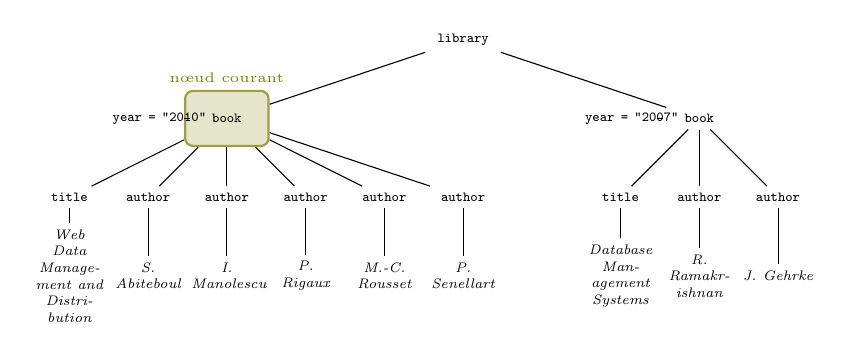
\begin{tikzpicture}[auto]
\tiny
  \tikzstyle{emptyStyle}=[text width=0.9cm, text centered]
  \tikzstyle{red}=[rounded corners=1mm,thick,draw=red!75,fill=red!20,text width=0.9cm, text centered]
  \tikzstyle{DarkViolet}=[rounded corners=1mm,thick,draw=DarkViolet!75,fill=DarkViolet!20,minimum size=7mm,text width=0.8cm, text centered]
  \tikzstyle{green}=[rounded corners=1mm,thick,draw=DarkOliveGreen!75,fill=DarkOliveGreen!20,minimum size=7mm,text width=0.8cm, text centered]
  \tikzstyle{cyan}=[rounded corners=1mm,thick,draw=DarkCyan!75,fill=DarkCyan!20,minimum size=7mm,text width=0.8cm, text centered]
 \tikzstyle{every label}=[black]
  \tikzstyle{HotPink}=[rounded corners=1mm,thick,draw=HotPink!75,fill=HotPink!20,minimum size=7mm,text width=0.8cm, text centered]
  \tikzstyle{noeudcourant}=[rounded corners=1mm,thick,draw=Olive!75,fill=Olive!20,minimum size=7mm,text width=0.9cm, text centered, label=\textcolor{Olive}{n{\oe}ud courant}]
  \tikzstyle{indiaRed}=[rounded corners=1mm,thick,draw=indiaRed!75,fill=indiaRed!20,minimum size=7mm,text width=0.9cm, text centered]

  \begin{scope}
   % \node[emptyStyle](r) at (7,5) {Root};  
   %\node[emptyStyle](entete) at (3,4) {\texttt{$<?xml$ version $...>$}};
   %\draw[-] (r) -- (entete);
   \node[emptyStyle](library) at (7,4) {\verb?library?};
   % \draw[-] (r) -- (library);

    \node[noeudcourant](book1) at (4,3) {\verb?book?};
   \draw[-] (library) -- (book1);
   \node[emptyStyle](book2) at (10,3) {\verb?book?};
   \draw[-] (library) -- (book2);

    \node[emptyStyle](year1) at (3,3) {\verb?year = "2010"?};
   \draw[-] (book1) -- (year1);
    \node[emptyStyle](title1) at (2,2) {\verb?title?};
   \draw[-] (book1) -- (title1);
 \node[emptyStyle](texttitle1) at (2,1) {\it Web Data Management and Distribution};
   \draw[-] (title1) -- (texttitle1);
    \node[emptyStyle](author1) at (3,2) {\verb?author?};
   \draw[-] (book1) -- (author1);
   \node[emptyStyle](textauthor1) at (3,1) {\it S. Abiteboul};
   \draw[-] (author1) -- (textauthor1);
    \node[emptyStyle](author2) at (4,2) {\verb?author?};
   \draw[-] (book1) -- (author2);
   \node[emptyStyle](textauthor2) at (4,1) {\it I. Manolescu};
   \draw[-] (author2) -- (textauthor2);
    \node[emptyStyle](author3) at (5,2) {\verb?author?};
   \draw[-] (book1) -- (author3);
   \node[emptyStyle](textauthor3) at (5,1) {\it P. Rigaux};
   \draw[-] (author3) -- (textauthor3);
    \node[emptyStyle](author4) at (6,2) {\verb?author?};
   \draw[-] (book1) -- (author4);
   \node[emptyStyle](textauthor4) at (6,1) {\it M.-C. Rousset};
   \draw[-] (author4) -- (textauthor4);
    \node[emptyStyle](author5) at (7,2) {\verb?author?};
   \draw[-] (book1) -- (author5);
   \node[emptyStyle](textauthor5) at (7,1) {\it P. Senellart};
   \draw[-] (author5) -- (textauthor5);

    \node[emptyStyle](year2) at (9,3) {\verb?year = "2007"?};
   \draw[-] (book2) -- (year2);
    \node[emptyStyle](title2) at (9,2) {\verb?title?};
   \draw[-] (book2) -- (title2);
 \node[emptyStyle](texttitle2) at (9,1) {\it Database Management Systems};
   \draw[-] (title2) -- (texttitle2);
    \node[emptyStyle](author1prime) at (10,2) {\verb?author?};
   \draw[-] (book2) -- (author1prime);
   \node[emptyStyle](textauthor1prime) at (10,1) {\it R. Ramakrishnan};
   \draw[-] (author1prime) -- (textauthor1prime);
    \node[emptyStyle](author2prime) at (11,2) {\verb?author?};
   \draw[-] (book2) -- (author2prime);
   \node[emptyStyle](textauthor2prime) at (11,1) {\it J. Gehrke};
   \draw[-] (author2prime) -- (textauthor2prime);
\end{scope}
\end{tikzpicture}
\end{frame}


 \begin{frame}{Quelques axes en exemple : Descendant}
\texttt{descendant} : Selects all descendants (children, grandchildren, etc.) of the current node

\bigskip

\begin{tikzpicture}[auto]
\tiny
  \tikzstyle{emptyStyle}=[text width=0.9cm, text centered]
  \tikzstyle{red}=[rounded corners=1mm,thick,draw=red!75,fill=red!20,text width=0.9cm, text centered]
  \tikzstyle{DarkViolet}=[rounded corners=1mm,thick,draw=DarkViolet!75,fill=DarkViolet!20,minimum size=7mm,text width=0.8cm, text centered]
  \tikzstyle{green}=[rounded corners=1mm,thick,draw=DarkOliveGreen!75,fill=DarkOliveGreen!20,minimum size=7mm,text width=0.8cm, text centered]
  \tikzstyle{cyan}=[rounded corners=1mm,thick,draw=DarkCyan!75,fill=DarkCyan!20,minimum size=7mm,text width=0.8cm, text centered]
 \tikzstyle{every label}=[black]
  \tikzstyle{HotPink}=[rounded corners=1mm,thick,draw=HotPink!75,fill=HotPink!20,minimum size=7mm,text width=0.8cm, text centered]
  \tikzstyle{noeudcourant}=[rounded corners=1mm,thick,draw=Olive!75,fill=Olive!20,minimum size=7mm,text width=0.9cm, text centered, label=\textcolor{Olive}{n{\oe}ud courant}]
  \tikzstyle{indiaRed}=[rounded corners=1mm,thick,draw=indiaRed!75,fill=indiaRed!20,minimum size=7mm,text width=0.9cm, text centered]

  \begin{scope}
   % \node[emptyStyle](r) at (7,5) {Root};  
   %\node[emptyStyle](entete) at (3,4) {\texttt{$<?xml$ version $...>$}};
   %\draw[-] (r) -- (entete);
   \node[emptyStyle](library) at (7,4) {\verb?library?};
   % \draw[-] (r) -- (library);

    \node[noeudcourant](book1) at (4,3) {\verb?book?};
   \draw[-] (library) -- (book1);
   \node[emptyStyle](book2) at (10,3) {\verb?book?};
   \draw[-] (library) -- (book2);

    \node[emptyStyle](year1) at (3,3) {\verb?year = "2010"?};
   \draw[-] (book1) -- (year1);
    \node[indiaRed](title1) at (2,2) {\verb?title?};
   \draw[-] (book1) -- (title1);
 \node[indiaRed](texttitle1) at (2,1) {\it Web Data Management and Distribution};
   \draw[-] (title1) -- (texttitle1);
    \node[indiaRed](author1) at (3,2) {\verb?author?};
   \draw[-] (book1) -- (author1);
   \node[indiaRed](textauthor1) at (3,1) {\it S. Abiteboul};
   \draw[-] (author1) -- (textauthor1);
    \node[indiaRed](author2) at (4,2) {\verb?author?};
   \draw[-] (book1) -- (author2);
   \node[indiaRed](textauthor2) at (4,1) {\it I. Manolescu};
   \draw[-] (author2) -- (textauthor2);
    \node[indiaRed](author3) at (5,2) {\verb?author?};
   \draw[-] (book1) -- (author3);
   \node[indiaRed](textauthor3) at (5,1) {\it P. Rigaux};
   \draw[-] (author3) -- (textauthor3);
    \node[indiaRed](author4) at (6,2) {\verb?author?};
   \draw[-] (book1) -- (author4);
   \node[indiaRed](textauthor4) at (6,1) {\it M.-C. Rousset};
   \draw[-] (author4) -- (textauthor4);
    \node[indiaRed](author5) at (7,2) {\verb?author?};
   \draw[-] (book1) -- (author5);
   \node[indiaRed](textauthor5) at (7,1) {\it P. Senellart};
   \draw[-] (author5) -- (textauthor5);

    \node[emptyStyle](year2) at (9,3) {\verb?year = "2007"?};
   \draw[-] (book2) -- (year2);
    \node[emptyStyle](title2) at (9,2) {\verb?title?};
   \draw[-] (book2) -- (title2);
 \node[emptyStyle](texttitle2) at (9,1) {\it Database Management Systems};
   \draw[-] (title2) -- (texttitle2);
    \node[emptyStyle](author1prime) at (10,2) {\verb?author?};
   \draw[-] (book2) -- (author1prime);
   \node[emptyStyle](textauthor1prime) at (10,1) {\it R. Ramakrishnan};
   \draw[-] (author1prime) -- (textauthor1prime);
    \node[emptyStyle](author2prime) at (11,2) {\verb?author?};
   \draw[-] (book2) -- (author2prime);
   \node[emptyStyle](textauthor2prime) at (11,1) {\it J. Gehrke};
   \draw[-] (author2prime) -- (textauthor2prime);
\end{scope}
\end{tikzpicture}
\end{frame}


\subsection{Descendant-or-self}

\begin{frame}{Quelques axes en exemple : Descendant-or-self}
\texttt{descendant-or-self} : Selects all descendants (children, grandchildren, etc.) of the current node and the current node itself

\bigskip

\begin{tikzpicture}[auto]
\tiny
  \tikzstyle{emptyStyle}=[text width=0.9cm, text centered]
  \tikzstyle{red}=[rounded corners=1mm,thick,draw=red!75,fill=red!20,text width=0.9cm, text centered]
  \tikzstyle{DarkViolet}=[rounded corners=1mm,thick,draw=DarkViolet!75,fill=DarkViolet!20,minimum size=7mm,text width=0.8cm, text centered]
  \tikzstyle{green}=[rounded corners=1mm,thick,draw=DarkOliveGreen!75,fill=DarkOliveGreen!20,minimum size=7mm,text width=0.8cm, text centered]
  \tikzstyle{cyan}=[rounded corners=1mm,thick,draw=DarkCyan!75,fill=DarkCyan!20,minimum size=7mm,text width=0.8cm, text centered]
 \tikzstyle{every label}=[black]
  \tikzstyle{HotPink}=[rounded corners=1mm,thick,draw=HotPink!75,fill=HotPink!20,minimum size=7mm,text width=0.8cm, text centered]
  \tikzstyle{noeudcourant}=[rounded corners=1mm,thick,draw=Olive!75,fill=Olive!20,minimum size=7mm,text width=0.9cm, text centered, label=\textcolor{Olive}{n{\oe}ud courant}]
  \tikzstyle{indiaRed}=[rounded corners=1mm,thick,draw=indiaRed!75,fill=indiaRed!20,minimum size=7mm,text width=0.9cm, text centered]

  \begin{scope}
   % \node[emptyStyle](r) at (7,5) {Root};  
   %\node[emptyStyle](entete) at (3,4) {\texttt{$<?xml$ version $...>$}};
   %\draw[-] (r) -- (entete);
   \node[emptyStyle](library) at (7,4) {\verb?library?};
   % \draw[-] (r) -- (library);

    \node[indiaRed,label=\textcolor{Olive}{n{\oe}ud courant}](book1) at (4,3) {\verb?book?};
   \draw[-] (library) -- (book1);
   \node[emptyStyle](book2) at (10,3) {\verb?book?};
   \draw[-] (library) -- (book2);

    \node[emptyStyle](year1) at (3,3) {\verb?year = "2010"?};
   \draw[-] (book1) -- (year1);
    \node[indiaRed](title1) at (2,2) {\verb?title?};
   \draw[-] (book1) -- (title1);
 \node[indiaRed](texttitle1) at (2,1) {\it Web Data Management and Distribution};
   \draw[-] (title1) -- (texttitle1);
    \node[indiaRed](author1) at (3,2) {\verb?author?};
   \draw[-] (book1) -- (author1);
   \node[indiaRed](textauthor1) at (3,1) {\it S. Abiteboul};
   \draw[-] (author1) -- (textauthor1);
    \node[indiaRed](author2) at (4,2) {\verb?author?};
   \draw[-] (book1) -- (author2);
   \node[indiaRed](textauthor2) at (4,1) {\it I. Manolescu};
   \draw[-] (author2) -- (textauthor2);
    \node[indiaRed](author3) at (5,2) {\verb?author?};
   \draw[-] (book1) -- (author3);
   \node[indiaRed](textauthor3) at (5,1) {\it P. Rigaux};
   \draw[-] (author3) -- (textauthor3);
    \node[indiaRed](author4) at (6,2) {\verb?author?};
   \draw[-] (book1) -- (author4);
   \node[indiaRed](textauthor4) at (6,1) {\it M.-C. Rousset};
   \draw[-] (author4) -- (textauthor4);
    \node[indiaRed](author5) at (7,2) {\verb?author?};
   \draw[-] (book1) -- (author5);
   \node[indiaRed](textauthor5) at (7,1) {\it P. Senellart};
   \draw[-] (author5) -- (textauthor5);

    \node[emptyStyle](year2) at (9,3) {\verb?year = "2007"?};
   \draw[-] (book2) -- (year2);
    \node[emptyStyle](title2) at (9,2) {\verb?title?};
   \draw[-] (book2) -- (title2);
 \node[emptyStyle](texttitle2) at (9,1) {\it Database Management Systems};
   \draw[-] (title2) -- (texttitle2);
    \node[emptyStyle](author1prime) at (10,2) {\verb?author?};
   \draw[-] (book2) -- (author1prime);
   \node[emptyStyle](textauthor1prime) at (10,1) {\it R. Ramakrishnan};
   \draw[-] (author1prime) -- (textauthor1prime);
    \node[emptyStyle](author2prime) at (11,2) {\verb?author?};
   \draw[-] (book2) -- (author2prime);
   \node[emptyStyle](textauthor2prime) at (11,1) {\it J. Gehrke};
   \draw[-] (author2prime) -- (textauthor2prime);
\end{scope}
\end{tikzpicture}

\end{frame}


\subsection{Following}
%following

 \begin{frame}{Quelques axes en exemple : Following}
\texttt{following} : Selects everything in the document defined after the closing tag of the current node

\bigskip

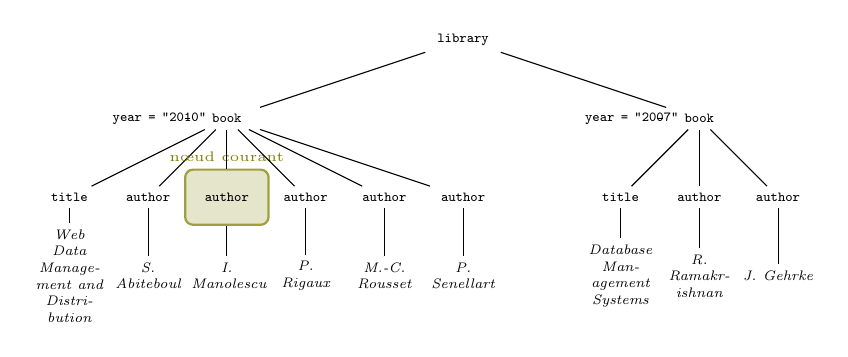
\begin{tikzpicture}[auto]
\tiny
  \tikzstyle{emptyStyle}=[text width=0.9cm, text centered]
  \tikzstyle{red}=[rounded corners=1mm,thick,draw=red!75,fill=red!20,text width=0.9cm, text centered]
  \tikzstyle{DarkViolet}=[rounded corners=1mm,thick,draw=DarkViolet!75,fill=DarkViolet!20,minimum size=7mm,text width=0.8cm, text centered]
  \tikzstyle{green}=[rounded corners=1mm,thick,draw=DarkOliveGreen!75,fill=DarkOliveGreen!20,minimum size=7mm,text width=0.8cm, text centered]
  \tikzstyle{cyan}=[rounded corners=1mm,thick,draw=DarkCyan!75,fill=DarkCyan!20,minimum size=7mm,text width=0.8cm, text centered]
 \tikzstyle{every label}=[black]
  \tikzstyle{HotPink}=[rounded corners=1mm,thick,draw=HotPink!75,fill=HotPink!20,minimum size=7mm,text width=0.8cm, text centered]
  \tikzstyle{noeudcourant}=[rounded corners=1mm,thick,draw=Olive!75,fill=Olive!20,minimum size=7mm,text width=0.9cm, text centered, label=\textcolor{Olive}{n{\oe}ud courant}]
  \tikzstyle{indiaRed}=[rounded corners=1mm,thick,draw=indiaRed!75,fill=indiaRed!20,minimum size=7mm,text width=0.9cm, text centered]

  \begin{scope}
   % \node[emptyStyle](r) at (7,5) {Root};  
   %\node[emptyStyle](entete) at (3,4) {\texttt{$<?xml$ version $...>$}};
   %\draw[-] (r) -- (entete);
   \node[emptyStyle](library) at (7,4) {\verb?library?};
   % \draw[-] (r) -- (library);

    \node[emptyStyle](book1) at (4,3) {\verb?book?};
   \draw[-] (library) -- (book1);
   \node[emptyStyle](book2) at (10,3) {\verb?book?};
   \draw[-] (library) -- (book2);

    \node[emptyStyle](year1) at (3,3) {\verb?year = "2010"?};
   \draw[-] (book1) -- (year1);
    \node[emptyStyle](title1) at (2,2) {\verb?title?};
   \draw[-] (book1) -- (title1);
 \node[emptyStyle](texttitle1) at (2,1) {\it Web Data Management and Distribution};
   \draw[-] (title1) -- (texttitle1);
    \node[emptyStyle](author1) at (3,2) {\verb?author?};
   \draw[-] (book1) -- (author1);
   \node[emptyStyle](textauthor1) at (3,1) {\it S. Abiteboul};
   \draw[-] (author1) -- (textauthor1);
    \node[noeudcourant](author2) at (4,2) {\verb?author?};
   \draw[-] (book1) -- (author2);
   \node[emptyStyle](textauthor2) at (4,1) {\it I. Manolescu};
   \draw[-] (author2) -- (textauthor2);
    \node[emptyStyle](author3) at (5,2) {\verb?author?};
   \draw[-] (book1) -- (author3);
   \node[emptyStyle](textauthor3) at (5,1) {\it P. Rigaux};
   \draw[-] (author3) -- (textauthor3);
    \node[emptyStyle](author4) at (6,2) {\verb?author?};
   \draw[-] (book1) -- (author4);
   \node[emptyStyle](textauthor4) at (6,1) {\it M.-C. Rousset};
   \draw[-] (author4) -- (textauthor4);
    \node[emptyStyle](author5) at (7,2) {\verb?author?};
   \draw[-] (book1) -- (author5);
   \node[emptyStyle](textauthor5) at (7,1) {\it P. Senellart};
   \draw[-] (author5) -- (textauthor5);

    \node[emptyStyle](year2) at (9,3) {\verb?year = "2007"?};
   \draw[-] (book2) -- (year2);
    \node[emptyStyle](title2) at (9,2) {\verb?title?};
   \draw[-] (book2) -- (title2);
 \node[emptyStyle](texttitle2) at (9,1) {\it Database Management Systems};
   \draw[-] (title2) -- (texttitle2);
    \node[emptyStyle](author1prime) at (10,2) {\verb?author?};
   \draw[-] (book2) -- (author1prime);
   \node[emptyStyle](textauthor1prime) at (10,1) {\it R. Ramakrishnan};
   \draw[-] (author1prime) -- (textauthor1prime);
    \node[emptyStyle](author2prime) at (11,2) {\verb?author?};
   \draw[-] (book2) -- (author2prime);
   \node[emptyStyle](textauthor2prime) at (11,1) {\it J. Gehrke};
   \draw[-] (author2prime) -- (textauthor2prime);
\end{scope}
\end{tikzpicture}

\end{frame}


\begin{frame}{Quelques axes en exemple : Following}
\texttt{following}  : Selects everything in the document defined after the closing tag of the current node
\bigskip
\lstinputlisting[basicstyle=\tiny, language=XML,breaklines=true, numbers=left, caption={Fichier twobooks.xml}]{codes/twobooks.xml}

\prof{1) Repérer le closing tag de author (ligne 6) et \\2) voir tous les elts définis après}
\end{frame}

\begin{frame}{Quelques axes en exemple : Following}
\texttt{following}  : Selects everything in the document defined after the closing tag of the current node

\bigskip

\begin{tikzpicture}[auto]
\tiny
  \tikzstyle{emptyStyle}=[text width=0.9cm, text centered]
  \tikzstyle{red}=[rounded corners=1mm,thick,draw=red!75,fill=red!20,text width=0.9cm, text centered]
  \tikzstyle{DarkViolet}=[rounded corners=1mm,thick,draw=DarkViolet!75,fill=DarkViolet!20,minimum size=7mm,text width=0.8cm, text centered]
  \tikzstyle{green}=[rounded corners=1mm,thick,draw=DarkOliveGreen!75,fill=DarkOliveGreen!20,minimum size=7mm,text width=0.8cm, text centered]
  \tikzstyle{cyan}=[rounded corners=1mm,thick,draw=DarkCyan!75,fill=DarkCyan!20,minimum size=7mm,text width=0.8cm, text centered]
 \tikzstyle{every label}=[black]
  \tikzstyle{HotPink}=[rounded corners=1mm,thick,draw=HotPink!75,fill=HotPink!20,minimum size=7mm,text width=0.8cm, text centered]
  \tikzstyle{noeudcourant}=[rounded corners=1mm,thick,draw=Olive!75,fill=Olive!20,minimum size=7mm,text width=0.9cm, text centered, label=\textcolor{Olive}{n{\oe}ud courant}]
  \tikzstyle{indiaRed}=[rounded corners=1mm,thick,draw=indiaRed!75,fill=indiaRed!20,minimum size=7mm,text width=0.9cm, text centered]

  \begin{scope}
   % \node[emptyStyle](r) at (7,5) {Root};  
   %\node[emptyStyle](entete) at (3,4) {\texttt{$<?xml$ version $...>$}};
   %\draw[-] (r) -- (entete);
   \node[emptyStyle](library) at (7,4) {\verb?library?};
   % \draw[-] (r) -- (library);

    \node[emptyStyle](book1) at (4,3) {\verb?book?};
   \draw[-] (library) -- (book1);
   \node[indiaRed](book2) at (10,3) {\verb?book?};
   \draw[-] (library) -- (book2);

    \node[emptyStyle](year1) at (3,3) {\verb?year = "2010"?};
   \draw[-] (book1) -- (year1);
    \node[emptyStyle](title1) at (2,2) {\verb?title?};
   \draw[-] (book1) -- (title1);
 \node[emptyStyle](texttitle1) at (2,1) {\it Web Data Management and Distribution};
   \draw[-] (title1) -- (texttitle1);
    \node[emptyStyle](author1) at (3,2) {\verb?author?};
   \draw[-] (book1) -- (author1);
   \node[emptyStyle](textauthor1) at (3,1) {\it S. Abiteboul};
   \draw[-] (author1) -- (textauthor1);
    \node[noeudcourant](author2) at (4,2) {\verb?author?};
   \draw[-] (book1) -- (author2);
   \node[emptyStyle](textauthor2) at (4,1) {\it I. Manolescu};
   \draw[-] (author2) -- (textauthor2);
    \node[indiaRed](author3) at (5,2) {\verb?author?};
   \draw[-] (book1) -- (author3);
   \node[indiaRed](textauthor3) at (5,1) {\it P. Rigaux};
   \draw[-] (author3) -- (textauthor3);
    \node[indiaRed](author4) at (6,2) {\verb?author?};
   \draw[-] (book1) -- (author4);
   \node[indiaRed](textauthor4) at (6,1) {\it M.-C. Rousset};
   \draw[-] (author4) -- (textauthor4);
    \node[indiaRed](author5) at (7,2) {\verb?author?};
   \draw[-] (book1) -- (author5);
   \node[indiaRed](textauthor5) at (7,1) {\it P. Senellart};
   \draw[-] (author5) -- (textauthor5);

    \node[indiaRed](year2) at (9,3) {\verb?year = "2007"?};
   \draw[-] (book2) -- (year2);
    \node[indiaRed](title2) at (9,2) {\verb?title?};
   \draw[-] (book2) -- (title2);
 \node[indiaRed](texttitle2) at (9,1) {\it Database Management Systems};
   \draw[-] (title2) -- (texttitle2);
    \node[indiaRed](author1prime) at (10,2) {\verb?author?};
   \draw[-] (book2) -- (author1prime);
   \node[indiaRed](textauthor1prime) at (10,1) {\it R. Ramakrishnan};
   \draw[-] (author1prime) -- (textauthor1prime);
    \node[indiaRed](author2prime) at (11,2) {\verb?author?};
   \draw[-] (book2) -- (author2prime);
   \node[indiaRed](textauthor2prime) at (11,1) {\it J. Gehrke};
   \draw[-] (author2prime) -- (textauthor2prime);
\end{scope}
\end{tikzpicture}

\end{frame}


%following-sibling
\subsection{Following-sibling}

 \begin{frame}{Quelques axes en exemple : Following-sibling}
\texttt{following-sibling} : Selects all siblings after the current node. \prof{sibling=fr\`ere ou s{\oe}ur}

\bigskip

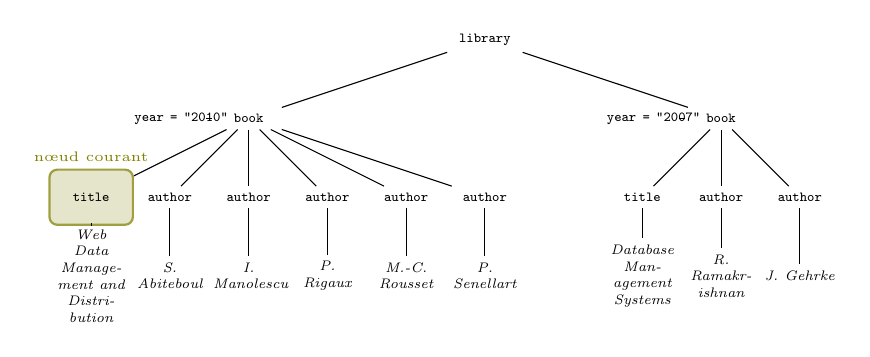
\begin{tikzpicture}[auto]
\tiny
  \tikzstyle{emptyStyle}=[text width=0.9cm, text centered]
  \tikzstyle{red}=[rounded corners=1mm,thick,draw=red!75,fill=red!20,text width=0.9cm, text centered]
  \tikzstyle{DarkViolet}=[rounded corners=1mm,thick,draw=DarkViolet!75,fill=DarkViolet!20,minimum size=7mm,text width=0.8cm, text centered]
  \tikzstyle{green}=[rounded corners=1mm,thick,draw=DarkOliveGreen!75,fill=DarkOliveGreen!20,minimum size=7mm,text width=0.8cm, text centered]
  \tikzstyle{cyan}=[rounded corners=1mm,thick,draw=DarkCyan!75,fill=DarkCyan!20,minimum size=7mm,text width=0.8cm, text centered]
 \tikzstyle{every label}=[black]
  \tikzstyle{HotPink}=[rounded corners=1mm,thick,draw=HotPink!75,fill=HotPink!20,minimum size=7mm,text width=0.8cm, text centered]
  \tikzstyle{noeudcourant}=[rounded corners=1mm,thick,draw=Olive!75,fill=Olive!20,minimum size=7mm,text width=0.9cm, text centered, label=\textcolor{Olive}{n{\oe}ud courant}]
  \tikzstyle{indiaRed}=[rounded corners=1mm,thick,draw=indiaRed!75,fill=indiaRed!20,minimum size=7mm,text width=0.9cm, text centered]

  \begin{scope}
   % \node[emptyStyle](r) at (7,5) {Root};  
   %\node[emptyStyle](entete) at (3,4) {\texttt{$<?xml$ version $...>$}};
   %\draw[-] (r) -- (entete);
   \node[emptyStyle](library) at (7,4) {\verb?library?};
   % \draw[-] (r) -- (library);

    \node[emptyStyle](book1) at (4,3) {\verb?book?};
   \draw[-] (library) -- (book1);
   \node[emptyStyle](book2) at (10,3) {\verb?book?};
   \draw[-] (library) -- (book2);

    \node[emptyStyle](year1) at (3,3) {\verb?year = "2010"?};
   \draw[-] (book1) -- (year1);
    \node[noeudcourant](title1) at (2,2) {\verb?title?};
   \draw[-] (book1) -- (title1);
 \node[emptyStyle](texttitle1) at (2,1) {\it Web Data Management and Distribution};
   \draw[-] (title1) -- (texttitle1);
    \node[emptyStyle](author1) at (3,2) {\verb?author?};
   \draw[-] (book1) -- (author1);
   \node[emptyStyle](textauthor1) at (3,1) {\it S. Abiteboul};
   \draw[-] (author1) -- (textauthor1);
    \node[emptyStyle](author2) at (4,2) {\verb?author?};
   \draw[-] (book1) -- (author2);
   \node[emptyStyle](textauthor2) at (4,1) {\it I. Manolescu};
   \draw[-] (author2) -- (textauthor2);
    \node[emptyStyle](author3) at (5,2) {\verb?author?};
   \draw[-] (book1) -- (author3);
   \node[emptyStyle](textauthor3) at (5,1) {\it P. Rigaux};
   \draw[-] (author3) -- (textauthor3);
    \node[emptyStyle](author4) at (6,2) {\verb?author?};
   \draw[-] (book1) -- (author4);
   \node[emptyStyle](textauthor4) at (6,1) {\it M.-C. Rousset};
   \draw[-] (author4) -- (textauthor4);
    \node[emptyStyle](author5) at (7,2) {\verb?author?};
   \draw[-] (book1) -- (author5);
   \node[emptyStyle](textauthor5) at (7,1) {\it P. Senellart};
   \draw[-] (author5) -- (textauthor5);

    \node[emptyStyle](year2) at (9,3) {\verb?year = "2007"?};
   \draw[-] (book2) -- (year2);
    \node[emptyStyle](title2) at (9,2) {\verb?title?};
   \draw[-] (book2) -- (title2);
 \node[emptyStyle](texttitle2) at (9,1) {\it Database Management Systems};
   \draw[-] (title2) -- (texttitle2);
    \node[emptyStyle](author1prime) at (10,2) {\verb?author?};
   \draw[-] (book2) -- (author1prime);
   \node[emptyStyle](textauthor1prime) at (10,1) {\it R. Ramakrishnan};
   \draw[-] (author1prime) -- (textauthor1prime);
    \node[emptyStyle](author2prime) at (11,2) {\verb?author?};
   \draw[-] (book2) -- (author2prime);
   \node[emptyStyle](textauthor2prime) at (11,1) {\it J. Gehrke};
   \draw[-] (author2prime) -- (textauthor2prime);
\end{scope}
\end{tikzpicture}




\end{frame}


 \begin{frame}{Quelques axes en exemple : Following-sibling}
\texttt{following-sibling} : Selects all siblings after the current node

\bigskip

\begin{tikzpicture}[auto]
\tiny
  \tikzstyle{emptyStyle}=[text width=0.9cm, text centered]
  \tikzstyle{red}=[rounded corners=1mm,thick,draw=red!75,fill=red!20,text width=0.9cm, text centered]
  \tikzstyle{DarkViolet}=[rounded corners=1mm,thick,draw=DarkViolet!75,fill=DarkViolet!20,minimum size=7mm,text width=0.8cm, text centered]
  \tikzstyle{green}=[rounded corners=1mm,thick,draw=DarkOliveGreen!75,fill=DarkOliveGreen!20,minimum size=7mm,text width=0.8cm, text centered]
  \tikzstyle{cyan}=[rounded corners=1mm,thick,draw=DarkCyan!75,fill=DarkCyan!20,minimum size=7mm,text width=0.8cm, text centered]
 \tikzstyle{every label}=[black]
  \tikzstyle{HotPink}=[rounded corners=1mm,thick,draw=HotPink!75,fill=HotPink!20,minimum size=7mm,text width=0.8cm, text centered]
  \tikzstyle{noeudcourant}=[rounded corners=1mm,thick,draw=Olive!75,fill=Olive!20,minimum size=7mm,text width=0.9cm, text centered, label=\textcolor{Olive}{n{\oe}ud courant}]
  \tikzstyle{indiaRed}=[rounded corners=1mm,thick,draw=indiaRed!75,fill=indiaRed!20,minimum size=7mm,text width=0.9cm, text centered]

  \begin{scope}
   % \node[emptyStyle](r) at (7,5) {Root};  
   %\node[emptyStyle](entete) at (3,4) {\texttt{$<?xml$ version $...>$}};
   %\draw[-] (r) -- (entete);
   \node[emptyStyle](library) at (7,4) {\verb?library?};
   % \draw[-] (r) -- (library);

    \node[emptyStyle](book1) at (4,3) {\verb?book?};
   \draw[-] (library) -- (book1);
   \node[emptyStyle](book2) at (10,3) {\verb?book?};
   \draw[-] (library) -- (book2);

    \node[emptyStyle](year1) at (3,3) {\verb?year = "2010"?};
   \draw[-] (book1) -- (year1);
    \node[noeudcourant](title1) at (2,2) {\verb?title?};
   \draw[-] (book1) -- (title1);
 \node[emptyStyle](texttitle1) at (2,1) {\it Web Data Management and Distribution};
   \draw[-] (title1) -- (texttitle1);
    \node[indiaRed](author1) at (3,2) {\verb?author?};
   \draw[-] (book1) -- (author1);
   \node[emptyStyle](textauthor1) at (3,1) {\it S. Abiteboul};
   \draw[-] (author1) -- (textauthor1);
    \node[indiaRed](author2) at (4,2) {\verb?author?};
   \draw[-] (book1) -- (author2);
   \node[emptyStyle](textauthor2) at (4,1) {\it I. Manolescu};
   \draw[-] (author2) -- (textauthor2);
    \node[indiaRed](author3) at (5,2) {\verb?author?};
   \draw[-] (book1) -- (author3);
   \node[emptyStyle](textauthor3) at (5,1) {\it P. Rigaux};
   \draw[-] (author3) -- (textauthor3);
    \node[indiaRed](author4) at (6,2) {\verb?author?};
   \draw[-] (book1) -- (author4);
   \node[emptyStyle](textauthor4) at (6,1) {\it M.-C. Rousset};
   \draw[-] (author4) -- (textauthor4);
    \node[indiaRed](author5) at (7,2) {\verb?author?};
   \draw[-] (book1) -- (author5);
   \node[emptyStyle](textauthor5) at (7,1) {\it P. Senellart};
   \draw[-] (author5) -- (textauthor5);

    \node[emptyStyle](year2) at (9,3) {\verb?year = "2007"?};
   \draw[-] (book2) -- (year2);
    \node[emptyStyle](title2) at (9,2) {\verb?title?};
   \draw[-] (book2) -- (title2);
 \node[emptyStyle](texttitle2) at (9,1) {\it Database Management Systems};
   \draw[-] (title2) -- (texttitle2);
    \node[emptyStyle](author1prime) at (10,2) {\verb?author?};
   \draw[-] (book2) -- (author1prime);
   \node[emptyStyle](textauthor1prime) at (10,1) {\it R. Ramakrishnan};
   \draw[-] (author1prime) -- (textauthor1prime);
    \node[emptyStyle](author2prime) at (11,2) {\verb?author?};
   \draw[-] (book2) -- (author2prime);
   \node[emptyStyle](textauthor2prime) at (11,1) {\it J. Gehrke};
   \draw[-] (author2prime) -- (textauthor2prime);
\end{scope}
\end{tikzpicture}

\end{frame}



\subsection{Preceding}
%Preceding

 \begin{frame}{Quelques axes en exemple : Following}
\texttt{preceding} : Selects everything in the document that is defined before the start tag of the current node

\bigskip

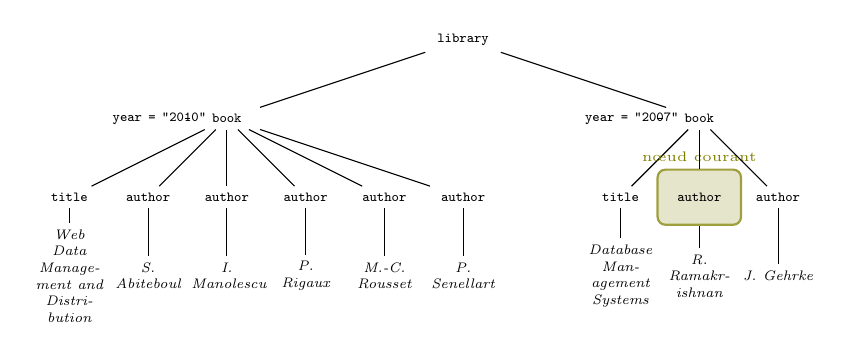
\begin{tikzpicture}[auto]
\tiny
  \tikzstyle{emptyStyle}=[text width=0.9cm, text centered]
  \tikzstyle{red}=[rounded corners=1mm,thick,draw=red!75,fill=red!20,text width=0.9cm, text centered]
  \tikzstyle{DarkViolet}=[rounded corners=1mm,thick,draw=DarkViolet!75,fill=DarkViolet!20,minimum size=7mm,text width=0.8cm, text centered]
  \tikzstyle{green}=[rounded corners=1mm,thick,draw=DarkOliveGreen!75,fill=DarkOliveGreen!20,minimum size=7mm,text width=0.8cm, text centered]
  \tikzstyle{cyan}=[rounded corners=1mm,thick,draw=DarkCyan!75,fill=DarkCyan!20,minimum size=7mm,text width=0.8cm, text centered]
 \tikzstyle{every label}=[black]
  \tikzstyle{HotPink}=[rounded corners=1mm,thick,draw=HotPink!75,fill=HotPink!20,minimum size=7mm,text width=0.8cm, text centered]
  \tikzstyle{noeudcourant}=[rounded corners=1mm,thick,draw=Olive!75,fill=Olive!20,minimum size=7mm,text width=0.9cm, text centered, label=\textcolor{Olive}{n{\oe}ud courant}]
  \tikzstyle{indiaRed}=[rounded corners=1mm,thick,draw=indiaRed!75,fill=indiaRed!20,minimum size=7mm,text width=0.9cm, text centered]

  \begin{scope}
   % \node[emptyStyle](r) at (7,5) {Root};  
   %\node[emptyStyle](entete) at (3,4) {\texttt{$<?xml$ version $...>$}};
   %\draw[-] (r) -- (entete);
   \node[emptyStyle](library) at (7,4) {\verb?library?};
   % \draw[-] (r) -- (library);

    \node[emptyStyle](book1) at (4,3) {\verb?book?};
   \draw[-] (library) -- (book1);
   \node[emptyStyle](book2) at (10,3) {\verb?book?};
   \draw[-] (library) -- (book2);

    \node[emptyStyle](year1) at (3,3) {\verb?year = "2010"?};
   \draw[-] (book1) -- (year1);
    \node[emptyStyle](title1) at (2,2) {\verb?title?};
   \draw[-] (book1) -- (title1);
 \node[emptyStyle](texttitle1) at (2,1) {\it Web Data Management and Distribution};
   \draw[-] (title1) -- (texttitle1);
    \node[emptyStyle](author1) at (3,2) {\verb?author?};
   \draw[-] (book1) -- (author1);
   \node[emptyStyle](textauthor1) at (3,1) {\it S. Abiteboul};
   \draw[-] (author1) -- (textauthor1);
    \node[emptyStyle](author2) at (4,2) {\verb?author?};
   \draw[-] (book1) -- (author2);
   \node[emptyStyle](textauthor2) at (4,1) {\it I. Manolescu};
   \draw[-] (author2) -- (textauthor2);
    \node[emptyStyle](author3) at (5,2) {\verb?author?};
   \draw[-] (book1) -- (author3);
   \node[emptyStyle](textauthor3) at (5,1) {\it P. Rigaux};
   \draw[-] (author3) -- (textauthor3);
    \node[emptyStyle](author4) at (6,2) {\verb?author?};
   \draw[-] (book1) -- (author4);
   \node[emptyStyle](textauthor4) at (6,1) {\it M.-C. Rousset};
   \draw[-] (author4) -- (textauthor4);
    \node[emptyStyle](author5) at (7,2) {\verb?author?};
   \draw[-] (book1) -- (author5);
   \node[emptyStyle](textauthor5) at (7,1) {\it P. Senellart};
   \draw[-] (author5) -- (textauthor5);

    \node[emptyStyle](year2) at (9,3) {\verb?year = "2007"?};
   \draw[-] (book2) -- (year2);
    \node[emptyStyle](title2) at (9,2) {\verb?title?};
   \draw[-] (book2) -- (title2);
 \node[emptyStyle](texttitle2) at (9,1) {\it Database Management Systems};
   \draw[-] (title2) -- (texttitle2);
    \node[noeudcourant](author1prime) at (10,2) {\verb?author?};
   \draw[-] (book2) -- (author1prime);
   \node[emptyStyle](textauthor1prime) at (10,1) {\it R. Ramakrishnan};
   \draw[-] (author1prime) -- (textauthor1prime);
    \node[emptyStyle](author2prime) at (11,2) {\verb?author?};
   \draw[-] (book2) -- (author2prime);
   \node[emptyStyle](textauthor2prime) at (11,1) {\it J. Gehrke};
   \draw[-] (author2prime) -- (textauthor2prime);
\end{scope}
\end{tikzpicture}

\end{frame}


\begin{frame}{Quelques axes en exemple : Following}
\texttt{preceding} : Selects everything in the document that is defined before the start tag of the current node
\bigskip
\lstinputlisting[basicstyle=\tiny, language=XML,breaklines=true, numbers=left, caption={Fichier twobooks.xml}]{codes/twobooks.xml}

\prof{1) Repérer le start tag de author Rama (ligne 13) et \\2) voir tous les elts définis avant}
\end{frame}

\begin{frame}{Quelques axes en exemple : Following}
\texttt{preceding} : Selects everything in the document that is defined before the start tag of the current node

\bigskip

\begin{tikzpicture}[auto]
\tiny
  \tikzstyle{emptyStyle}=[text width=0.9cm, text centered]
  \tikzstyle{red}=[rounded corners=1mm,thick,draw=red!75,fill=red!20,text width=0.9cm, text centered]
  \tikzstyle{DarkViolet}=[rounded corners=1mm,thick,draw=DarkViolet!75,fill=DarkViolet!20,minimum size=7mm,text width=0.8cm, text centered]
  \tikzstyle{green}=[rounded corners=1mm,thick,draw=DarkOliveGreen!75,fill=DarkOliveGreen!20,minimum size=7mm,text width=0.8cm, text centered]
  \tikzstyle{cyan}=[rounded corners=1mm,thick,draw=DarkCyan!75,fill=DarkCyan!20,minimum size=7mm,text width=0.8cm, text centered]
 \tikzstyle{every label}=[black]
  \tikzstyle{HotPink}=[rounded corners=1mm,thick,draw=HotPink!75,fill=HotPink!20,minimum size=7mm,text width=0.8cm, text centered]
  \tikzstyle{noeudcourant}=[rounded corners=1mm,thick,draw=Olive!75,fill=Olive!20,minimum size=7mm,text width=0.9cm, text centered, label=\textcolor{Olive}{n{\oe}ud courant}]
  \tikzstyle{indiaRed}=[rounded corners=1mm,thick,draw=indiaRed!75,fill=indiaRed!20,minimum size=7mm,text width=0.9cm, text centered]

  \begin{scope}
   % \node[emptyStyle](r) at (7,5) {Root};  
   %\node[emptyStyle](entete) at (3,4) {\texttt{$<?xml$ version $...>$}};
   %\draw[-] (r) -- (entete);
   \node[emptyStyle](library) at (7,4) {\verb?library?};
   % \draw[-] (r) -- (library);

    \node[indiaRed](book1) at (4,3) {\verb?book?};
   \draw[-] (library) -- (book1);
   \node[emptyStyle](book2) at (10,3) {\verb?book?};
   \draw[-] (library) -- (book2);

    \node[indiaRed](year1) at (3,3) {\verb?year = "2010"?};
   \draw[-] (book1) -- (year1);
    \node[indiaRed](title1) at (2,2) {\verb?title?};
   \draw[-] (book1) -- (title1);
 \node[indiaRed](texttitle1) at (2,1) {\it Web Data Management and Distribution};
   \draw[-] (title1) -- (texttitle1);
    \node[indiaRed](author1) at (3,2) {\verb?author?};
   \draw[-] (book1) -- (author1);
   \node[indiaRed](textauthor1) at (3,1) {\it S. Abiteboul};
   \draw[-] (author1) -- (textauthor1);
    \node[indiaRed](author2) at (4,2) {\verb?author?};
   \draw[-] (book1) -- (author2);
   \node[indiaRed](textauthor2) at (4,1) {\it I. Manolescu};
   \draw[-] (author2) -- (textauthor2);
    \node[indiaRed](author3) at (5,2) {\verb?author?};
   \draw[-] (book1) -- (author3);
   \node[indiaRed](textauthor3) at (5,1) {\it P. Rigaux};
   \draw[-] (author3) -- (textauthor3);
    \node[indiaRed](author4) at (6,2) {\verb?author?};
   \draw[-] (book1) -- (author4);
   \node[indiaRed](textauthor4) at (6,1) {\it M.-C. Rousset};
   \draw[-] (author4) -- (textauthor4);
    \node[indiaRed](author5) at (7,2) {\verb?author?};
   \draw[-] (book1) -- (author5);
   \node[indiaRed](textauthor5) at (7,1) {\it P. Senellart};
   \draw[-] (author5) -- (textauthor5);

    \node[emptyStyle](year2) at (9,3) {\verb?year = "2007"?};
   \draw[-] (book2) -- (year2);
    \node[indiaRed](title2) at (9,2) {\verb?title?};
   \draw[-] (book2) -- (title2);
 \node[indiaRed](texttitle2) at (9,1) {\it Database Management Systems};
   \draw[-] (title2) -- (texttitle2);
    \node[noeudcourant](author1prime) at (10,2) {\verb?author?};
   \draw[-] (book2) -- (author1prime);
   \node[emptyStyle](textauthor1prime) at (10,1) {\it R. Ramakrishnan};
   \draw[-] (author1prime) -- (textauthor1prime);
    \node[emptyStyle](author2prime) at (11,2) {\verb?author?};
   \draw[-] (book2) -- (author2prime);
   \node[emptyStyle](textauthor2prime) at (11,1) {\it J. Gehrke};
   \draw[-] (author2prime) -- (textauthor2prime);
\end{scope}
\end{tikzpicture}

\end{frame}

%preceding-sibling
\subsection{Preceding-sibling}

 \begin{frame}{Quelques axes en exemple : Following-sibling}
\texttt{preceding-sibling} : Selects all siblings before the current node. \prof{sibling=fr\`ere ou s{\oe}ur}

\bigskip

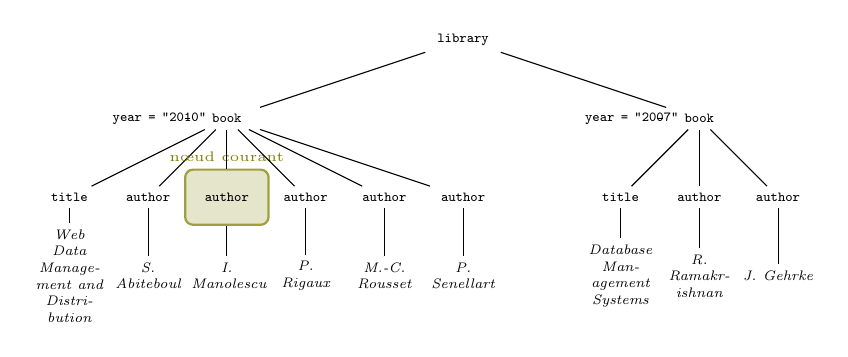
\begin{tikzpicture}[auto]
\tiny
  \tikzstyle{emptyStyle}=[text width=0.9cm, text centered]
  \tikzstyle{red}=[rounded corners=1mm,thick,draw=red!75,fill=red!20,text width=0.9cm, text centered]
  \tikzstyle{DarkViolet}=[rounded corners=1mm,thick,draw=DarkViolet!75,fill=DarkViolet!20,minimum size=7mm,text width=0.8cm, text centered]
  \tikzstyle{green}=[rounded corners=1mm,thick,draw=DarkOliveGreen!75,fill=DarkOliveGreen!20,minimum size=7mm,text width=0.8cm, text centered]
  \tikzstyle{cyan}=[rounded corners=1mm,thick,draw=DarkCyan!75,fill=DarkCyan!20,minimum size=7mm,text width=0.8cm, text centered]
 \tikzstyle{every label}=[black]
  \tikzstyle{HotPink}=[rounded corners=1mm,thick,draw=HotPink!75,fill=HotPink!20,minimum size=7mm,text width=0.8cm, text centered]
  \tikzstyle{noeudcourant}=[rounded corners=1mm,thick,draw=Olive!75,fill=Olive!20,minimum size=7mm,text width=0.9cm, text centered, label=\textcolor{Olive}{n{\oe}ud courant}]
  \tikzstyle{indiaRed}=[rounded corners=1mm,thick,draw=indiaRed!75,fill=indiaRed!20,minimum size=7mm,text width=0.9cm, text centered]

  \begin{scope}
   % \node[emptyStyle](r) at (7,5) {Root};  
   %\node[emptyStyle](entete) at (3,4) {\texttt{$<?xml$ version $...>$}};
   %\draw[-] (r) -- (entete);
   \node[emptyStyle](library) at (7,4) {\verb?library?};
   % \draw[-] (r) -- (library);

    \node[emptyStyle](book1) at (4,3) {\verb?book?};
   \draw[-] (library) -- (book1);
   \node[emptyStyle](book2) at (10,3) {\verb?book?};
   \draw[-] (library) -- (book2);

    \node[emptyStyle](year1) at (3,3) {\verb?year = "2010"?};
   \draw[-] (book1) -- (year1);
    \node[emptyStyle](title1) at (2,2) {\verb?title?};
   \draw[-] (book1) -- (title1);
 \node[emptyStyle](texttitle1) at (2,1) {\it Web Data Management and Distribution};
   \draw[-] (title1) -- (texttitle1);
    \node[emptyStyle](author1) at (3,2) {\verb?author?};
   \draw[-] (book1) -- (author1);
   \node[emptyStyle](textauthor1) at (3,1) {\it S. Abiteboul};
   \draw[-] (author1) -- (textauthor1);
    \node[noeudcourant](author2) at (4,2) {\verb?author?};
   \draw[-] (book1) -- (author2);
   \node[emptyStyle](textauthor2) at (4,1) {\it I. Manolescu};
   \draw[-] (author2) -- (textauthor2);
    \node[emptyStyle](author3) at (5,2) {\verb?author?};
   \draw[-] (book1) -- (author3);
   \node[emptyStyle](textauthor3) at (5,1) {\it P. Rigaux};
   \draw[-] (author3) -- (textauthor3);
    \node[emptyStyle](author4) at (6,2) {\verb?author?};
   \draw[-] (book1) -- (author4);
   \node[emptyStyle](textauthor4) at (6,1) {\it M.-C. Rousset};
   \draw[-] (author4) -- (textauthor4);
    \node[emptyStyle](author5) at (7,2) {\verb?author?};
   \draw[-] (book1) -- (author5);
   \node[emptyStyle](textauthor5) at (7,1) {\it P. Senellart};
   \draw[-] (author5) -- (textauthor5);

    \node[emptyStyle](year2) at (9,3) {\verb?year = "2007"?};
   \draw[-] (book2) -- (year2);
    \node[emptyStyle](title2) at (9,2) {\verb?title?};
   \draw[-] (book2) -- (title2);
 \node[emptyStyle](texttitle2) at (9,1) {\it Database Management Systems};
   \draw[-] (title2) -- (texttitle2);
    \node[emptyStyle](author1prime) at (10,2) {\verb?author?};
   \draw[-] (book2) -- (author1prime);
   \node[emptyStyle](textauthor1prime) at (10,1) {\it R. Ramakrishnan};
   \draw[-] (author1prime) -- (textauthor1prime);
    \node[emptyStyle](author2prime) at (11,2) {\verb?author?};
   \draw[-] (book2) -- (author2prime);
   \node[emptyStyle](textauthor2prime) at (11,1) {\it J. Gehrke};
   \draw[-] (author2prime) -- (textauthor2prime);
\end{scope}
\end{tikzpicture}

\end{frame}


 \begin{frame}{Quelques axes en exemple : Following-sibling}
\texttt{preceding-sibling} : Selects all siblings before the current node. \prof{sibling=fr\`ere ou s{\oe}ur}

\bigskip

\begin{tikzpicture}[auto]
\tiny
  \tikzstyle{emptyStyle}=[text width=0.9cm, text centered]
  \tikzstyle{red}=[rounded corners=1mm,thick,draw=red!75,fill=red!20,text width=0.9cm, text centered]
  \tikzstyle{DarkViolet}=[rounded corners=1mm,thick,draw=DarkViolet!75,fill=DarkViolet!20,minimum size=7mm,text width=0.8cm, text centered]
  \tikzstyle{green}=[rounded corners=1mm,thick,draw=DarkOliveGreen!75,fill=DarkOliveGreen!20,minimum size=7mm,text width=0.8cm, text centered]
  \tikzstyle{cyan}=[rounded corners=1mm,thick,draw=DarkCyan!75,fill=DarkCyan!20,minimum size=7mm,text width=0.8cm, text centered]
 \tikzstyle{every label}=[black]
  \tikzstyle{HotPink}=[rounded corners=1mm,thick,draw=HotPink!75,fill=HotPink!20,minimum size=7mm,text width=0.8cm, text centered]
  \tikzstyle{noeudcourant}=[rounded corners=1mm,thick,draw=Olive!75,fill=Olive!20,minimum size=7mm,text width=0.9cm, text centered, label=\textcolor{Olive}{n{\oe}ud courant}]
  \tikzstyle{indiaRed}=[rounded corners=1mm,thick,draw=indiaRed!75,fill=indiaRed!20,minimum size=7mm,text width=0.9cm, text centered]

  \begin{scope}
   % \node[emptyStyle](r) at (7,5) {Root};  
   %\node[emptyStyle](entete) at (3,4) {\texttt{$<?xml$ version $...>$}};
   %\draw[-] (r) -- (entete);
   \node[emptyStyle](library) at (7,4) {\verb?library?};
   % \draw[-] (r) -- (library);

    \node[emptyStyle](book1) at (4,3) {\verb?book?};
   \draw[-] (library) -- (book1);
   \node[emptyStyle](book2) at (10,3) {\verb?book?};
   \draw[-] (library) -- (book2);

    \node[emptyStyle](year1) at (3,3) {\verb?year = "2010"?};
   \draw[-] (book1) -- (year1);
    \node[indiaRed](title1) at (2,2) {\verb?title?};
   \draw[-] (book1) -- (title1);
 \node[emptyStyle](texttitle1) at (2,1) {\it Web Data Management and Distribution};
   \draw[-] (title1) -- (texttitle1);
    \node[indiaRed](author1) at (3,2) {\verb?author?};
   \draw[-] (book1) -- (author1);
   \node[emptyStyle](textauthor1) at (3,1) {\it S. Abiteboul};

   \draw[-] (author1) -- (textauthor1);
    \node[noeudcourant](author2) at (4,2) {\verb?author?};
   \draw[-] (book1) -- (author2);
   \node[emptyStyle](textauthor2) at (4,1) {\it I. Manolescu};
   \draw[-] (author2) -- (textauthor2);
    \node[emptyStyle](author3) at (5,2) {\verb?author?};
   \draw[-] (book1) -- (author3);
   \node[emptyStyle](textauthor3) at (5,1) {\it P. Rigaux};
   \draw[-] (author3) -- (textauthor3);
    \node[emptyStyle](author4) at (6,2) {\verb?author?};
   \draw[-] (book1) -- (author4);
   \node[emptyStyle](textauthor4) at (6,1) {\it M.-C. Rousset};
   \draw[-] (author4) -- (textauthor4);
    \node[emptyStyle](author5) at (7,2) {\verb?author?};
   \draw[-] (book1) -- (author5);
   \node[emptyStyle](textauthor5) at (7,1) {\it P. Senellart};
   \draw[-] (author5) -- (textauthor5);

    \node[emptyStyle](year2) at (9,3) {\verb?year = "2007"?};
   \draw[-] (book2) -- (year2);
    \node[emptyStyle](title2) at (9,2) {\verb?title?};
   \draw[-] (book2) -- (title2);
 \node[emptyStyle](texttitle2) at (9,1) {\it Database Management Systems};
   \draw[-] (title2) -- (texttitle2);
    \node[emptyStyle](author1prime) at (10,2) {\verb?author?};
   \draw[-] (book2) -- (author1prime);
   \node[emptyStyle](textauthor1prime) at (10,1) {\it R. Ramakrishnan};
   \draw[-] (author1prime) -- (textauthor1prime);
    \node[emptyStyle](author2prime) at (11,2) {\verb?author?};
   \draw[-] (book2) -- (author2prime);
   \node[emptyStyle](textauthor2prime) at (11,1) {\it J. Gehrke};
   \draw[-] (author2prime) -- (textauthor2prime);
\end{scope}
\end{tikzpicture}

\end{frame}



\subsection{Attribute}
%attribute

 \begin{frame}{Quelques axes en exemple : Attribute}
\texttt{attribute} : Selects all attributes of the current node

\bigskip

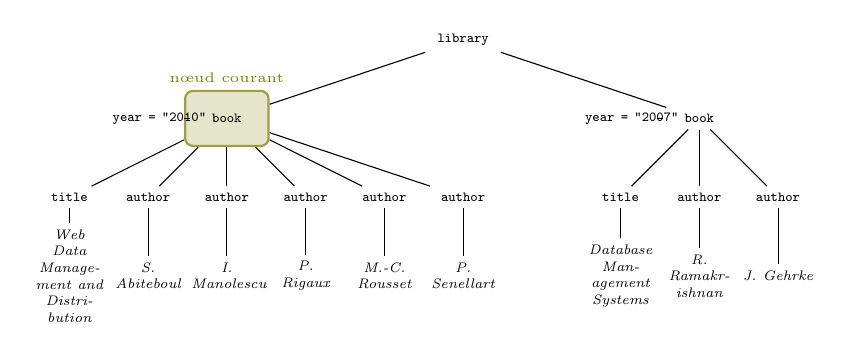
\begin{tikzpicture}[auto]
\tiny
  \tikzstyle{emptyStyle}=[text width=0.9cm, text centered]
  \tikzstyle{red}=[rounded corners=1mm,thick,draw=red!75,fill=red!20,text width=0.9cm, text centered]
  \tikzstyle{DarkViolet}=[rounded corners=1mm,thick,draw=DarkViolet!75,fill=DarkViolet!20,minimum size=7mm,text width=0.8cm, text centered]
  \tikzstyle{green}=[rounded corners=1mm,thick,draw=DarkOliveGreen!75,fill=DarkOliveGreen!20,minimum size=7mm,text width=0.8cm, text centered]
  \tikzstyle{cyan}=[rounded corners=1mm,thick,draw=DarkCyan!75,fill=DarkCyan!20,minimum size=7mm,text width=0.8cm, text centered]
 \tikzstyle{every label}=[black]
  \tikzstyle{HotPink}=[rounded corners=1mm,thick,draw=HotPink!75,fill=HotPink!20,minimum size=7mm,text width=0.8cm, text centered]
  \tikzstyle{noeudcourant}=[rounded corners=1mm,thick,draw=Olive!75,fill=Olive!20,minimum size=7mm,text width=0.9cm, text centered, label=\textcolor{Olive}{n{\oe}ud courant}]
  \tikzstyle{indiaRed}=[rounded corners=1mm,thick,draw=indiaRed!75,fill=indiaRed!20,minimum size=7mm,text width=0.9cm, text centered]

  \begin{scope}
   % \node[emptyStyle](r) at (7,5) {Root};  
   %\node[emptyStyle](entete) at (3,4) {\texttt{$<?xml$ version $...>$}};
   %\draw[-] (r) -- (entete);
   \node[emptyStyle](library) at (7,4) {\verb?library?};
   % \draw[-] (r) -- (library);

    \node[noeudcourant](book1) at (4,3) {\verb?book?};
   \draw[-] (library) -- (book1);
   \node[emptyStyle](book2) at (10,3) {\verb?book?};
   \draw[-] (library) -- (book2);

    \node[emptyStyle](year1) at (3,3) {\verb?year = "2010"?};
   \draw[-] (book1) -- (year1);
    \node[emptyStyle](title1) at (2,2) {\verb?title?};
   \draw[-] (book1) -- (title1);
 \node[emptyStyle](texttitle1) at (2,1) {\it Web Data Management and Distribution};
   \draw[-] (title1) -- (texttitle1);
    \node[emptyStyle](author1) at (3,2) {\verb?author?};
   \draw[-] (book1) -- (author1);
   \node[emptyStyle](textauthor1) at (3,1) {\it S. Abiteboul};
   \draw[-] (author1) -- (textauthor1);
    \node[emptyStyle](author2) at (4,2) {\verb?author?};
   \draw[-] (book1) -- (author2);
   \node[emptyStyle](textauthor2) at (4,1) {\it I. Manolescu};
   \draw[-] (author2) -- (textauthor2);
    \node[emptyStyle](author3) at (5,2) {\verb?author?};
   \draw[-] (book1) -- (author3);
   \node[emptyStyle](textauthor3) at (5,1) {\it P. Rigaux};
   \draw[-] (author3) -- (textauthor3);
    \node[emptyStyle](author4) at (6,2) {\verb?author?};
   \draw[-] (book1) -- (author4);
   \node[emptyStyle](textauthor4) at (6,1) {\it M.-C. Rousset};
   \draw[-] (author4) -- (textauthor4);
    \node[emptyStyle](author5) at (7,2) {\verb?author?};
   \draw[-] (book1) -- (author5);
   \node[emptyStyle](textauthor5) at (7,1) {\it P. Senellart};
   \draw[-] (author5) -- (textauthor5);

    \node[emptyStyle](year2) at (9,3) {\verb?year = "2007"?};
   \draw[-] (book2) -- (year2);
    \node[emptyStyle](title2) at (9,2) {\verb?title?};
   \draw[-] (book2) -- (title2);
 \node[emptyStyle](texttitle2) at (9,1) {\it Database Management Systems};
   \draw[-] (title2) -- (texttitle2);
    \node[emptyStyle](author1prime) at (10,2) {\verb?author?};
   \draw[-] (book2) -- (author1prime);
   \node[emptyStyle](textauthor1prime) at (10,1) {\it R. Ramakrishnan};
   \draw[-] (author1prime) -- (textauthor1prime);
    \node[emptyStyle](author2prime) at (11,2) {\verb?author?};
   \draw[-] (book2) -- (author2prime);
   \node[emptyStyle](textauthor2prime) at (11,1) {\it J. Gehrke};
   \draw[-] (author2prime) -- (textauthor2prime);
\end{scope}
\end{tikzpicture}




\end{frame}


 \begin{frame}{Quelques axes en exemple : Attribute}
\texttt{attribute} : Selects all attributes of the current node

\bigskip

\begin{tikzpicture}[auto]
\tiny
  \tikzstyle{emptyStyle}=[text width=0.9cm, text centered]
  \tikzstyle{red}=[rounded corners=1mm,thick,draw=red!75,fill=red!20,text width=0.9cm, text centered]
  \tikzstyle{DarkViolet}=[rounded corners=1mm,thick,draw=DarkViolet!75,fill=DarkViolet!20,minimum size=7mm,text width=0.8cm, text centered]
  \tikzstyle{green}=[rounded corners=1mm,thick,draw=DarkOliveGreen!75,fill=DarkOliveGreen!20,minimum size=7mm,text width=0.8cm, text centered]
  \tikzstyle{cyan}=[rounded corners=1mm,thick,draw=DarkCyan!75,fill=DarkCyan!20,minimum size=7mm,text width=0.8cm, text centered]
 \tikzstyle{every label}=[black]
  \tikzstyle{HotPink}=[rounded corners=1mm,thick,draw=HotPink!75,fill=HotPink!20,minimum size=7mm,text width=0.8cm, text centered]
  \tikzstyle{noeudcourant}=[rounded corners=1mm,thick,draw=Olive!75,fill=Olive!20,minimum size=7mm,text width=0.9cm, text centered, label=\textcolor{Olive}{n{\oe}ud courant}]
  \tikzstyle{indiaRed}=[rounded corners=1mm,thick,draw=indiaRed!75,fill=indiaRed!20,minimum size=7mm,text width=0.9cm, text centered]

  \begin{scope}
   % \node[emptyStyle](r) at (7,5) {Root};  
   %\node[emptyStyle](entete) at (3,4) {\texttt{$<?xml$ version $...>$}};
   %\draw[-] (r) -- (entete);
   \node[emptyStyle](library) at (7,4) {\verb?library?};
   % \draw[-] (r) -- (library);

    \node[noeudcourant](book1) at (4,3) {\verb?book?};
   \draw[-] (library) -- (book1);
   \node[emptyStyle](book2) at (10,3) {\verb?book?};
   \draw[-] (library) -- (book2);

    \node[indiaRed](year1) at (3,3) {\verb?year = "2010"?};
   \draw[-] (book1) -- (year1);
    \node[emptyStyle](title1) at (2,2) {\verb?title?};
   \draw[-] (book1) -- (title1);
 \node[emptyStyle](texttitle1) at (2,1) {\it Web Data Management and Distribution};
   \draw[-] (title1) -- (texttitle1);
    \node[emptyStyle](author1) at (3,2) {\verb?author?};
   \draw[-] (book1) -- (author1);
   \node[emptyStyle](textauthor1) at (3,1) {\it S. Abiteboul};
   \draw[-] (author1) -- (textauthor1);
    \node[emptyStyle](author2) at (4,2) {\verb?author?};
   \draw[-] (book1) -- (author2);
   \node[emptyStyle](textauthor2) at (4,1) {\it I. Manolescu};
   \draw[-] (author2) -- (textauthor2);
    \node[emptyStyle](author3) at (5,2) {\verb?author?};
   \draw[-] (book1) -- (author3);
   \node[emptyStyle](textauthor3) at (5,1) {\it P. Rigaux};
   \draw[-] (author3) -- (textauthor3);
    \node[emptyStyle](author4) at (6,2) {\verb?author?};
   \draw[-] (book1) -- (author4);
   \node[emptyStyle](textauthor4) at (6,1) {\it M.-C. Rousset};
   \draw[-] (author4) -- (textauthor4);
    \node[emptyStyle](author5) at (7,2) {\verb?author?};
   \draw[-] (book1) -- (author5);
   \node[emptyStyle](textauthor5) at (7,1) {\it P. Senellart};
   \draw[-] (author5) -- (textauthor5);

    \node[emptyStyle](year2) at (9,3) {\verb?year = "2007"?};
   \draw[-] (book2) -- (year2);
    \node[emptyStyle](title2) at (9,2) {\verb?title?};
   \draw[-] (book2) -- (title2);
 \node[emptyStyle](texttitle2) at (9,1) {\it Database Management Systems};
   \draw[-] (title2) -- (texttitle2);
    \node[emptyStyle](author1prime) at (10,2) {\verb?author?};
   \draw[-] (book2) -- (author1prime);
   \node[emptyStyle](textauthor1prime) at (10,1) {\it R. Ramakrishnan};
   \draw[-] (author1prime) -- (textauthor1prime);
    \node[emptyStyle](author2prime) at (11,2) {\verb?author?};
   \draw[-] (book2) -- (author2prime);
   \node[emptyStyle](textauthor2prime) at (11,1) {\it J. Gehrke};
   \draw[-] (author2prime) -- (textauthor2prime);
\end{scope}
\end{tikzpicture}

\end{frame}



\begin{frame}[allowframebreaks]{Exemple}

%\begin{center}
%\begin{minipage}{0.7\textwidth}
%\lstinputlisting[basicstyle=\tiny, language=XML,breaklines=true, caption={Un simple fichier XML}]{codes/livresExXpath.xml}
%\end{minipage}
%\end{center}

%\framebreak

\texttt{/child::library/child::*/attribute::year}

\begin{center}
\begin{tikzpicture}[auto]
\tiny
  \tikzstyle{emptyStyle}=[text width=0.9cm, text centered]
  \tikzstyle{parser}=[rounded corners=3mm,thick,draw=DarkViolet!75,fill=DarkViolet!20,,text centered]
  \tikzstyle{appli}=[rounded corners=1mm,thick,draw=red!75,fill=red!20,text centered,text width=2cm]
  \tikzstyle{every label}=[black]

  \begin{scope}
    \node[emptyStyle](r) at (6,5) {Root};
   \node[emptyStyle](comment) at (1,4) {\texttt{\verb?<!-- ceci ... >?}};
   \draw[-] (r) -- (comment);
    %\node[emptyStyle](entete) at (3,4) {\texttt{$<?xml$ version $...>$}};
   %\draw[-] (r) -- (entete);
    \node[emptyStyle](library) at (6,4) {\verb?<library> ... </library>?};
   \draw[-] (r) -- (library);

    \node[emptyStyle](book1) at (3,3) {\verb?<book> ... </book>?};
   \draw[-] (library) -- (book1);
    \node[emptyStyle](book2) at (6,3) {\verb?<book> ... </book>?};
   \draw[-] (library) -- (book2);
    \node[emptyStyle](book3) at (10,3) {\verb?<book> ... </book>?};
   \draw[-] (library) -- (book3);

    \node[emptyStyle](year1) at (2,3) {\verb?year = "1857"?};
   \draw[-] (book1) -- (year1);
    \node[emptyStyle](author1) at (2,2) {\verb?<author> ... </author>?};
   \draw[-] (book1) -- (author1);
    \node[emptyStyle](textauthor1) at (2,1) {\it Charles Baudelaire};
   \draw[-] (author1) -- (textauthor1);
    \node[emptyStyle](title1) at (3,2) {\verb?<title> ... </title>?};
   \draw[-] (book1) -- (title1);
    \node[emptyStyle](texttitle1) at (3,1) {\it Les fleurs du mal};
   \draw[-] (title1) -- (texttitle1);

    \node[emptyStyle](year2) at (5,3) {\verb?year = "1862"?};
   \draw[-] (book2) -- (year2);
    \node[emptyStyle](author2) at (6,2) {\verb?<author> ... </author>?};
   \draw[-] (book2) -- (author2);
    \node[emptyStyle](textauthor2) at (6,1) {\it Victor Hugo};
   \draw[-] (author2) -- (textauthor2);
    \node[emptyStyle](ln2) at (5,2) {\verb?ln = "Besancon"?};
   \draw[-] (author2) -- (ln2);
    \node[emptyStyle](title2) at (7,2) {\verb?<title> ... </title>?};
   \draw[-] (book2) -- (title2);
    \node[emptyStyle](texttitle2) at (7,1) {\it Les miserables};
   \draw[-] (title2) -- (texttitle2);

    \node[emptyStyle](year3) at (9,3) {\verb?year = "1877"?};
   \draw[-] (book3) -- (year3);
    \node[emptyStyle](author3) at (10,2) {\verb?<author> ... </author>?};
   \draw[-] (book3) -- (author3);
    \node[emptyStyle](textauthor3) at (10,1) {\it Emile Zola};
   \draw[-] (author3) -- (textauthor3);
    \node[emptyStyle](ln3) at (9,2) {\verb?ln = "Paris"?};
   \draw[-] (author3) -- (ln3);
    \node[emptyStyle](title3) at (11,2) {\verb?<title> ... </title>?};
   \draw[-] (book3) -- (title3);
    \node[emptyStyle](texttitle3) at (11,1) {\it L'assomoir};
   \draw[-] (title3) -- (texttitle3);

\end{scope}

%  \begin{pgfonlayer}{background}
%    \filldraw [line width=4mm,join=round,black!20]
%      (parser.north  -| parser.west)  rectangle (serial.south  -| serial.east);
%\end{pgfonlayer}


\end{tikzpicture}
\end{center}

\framebreak

\texttt{\textcolor{red}{\bf /}child::library/child::*/attribute::year}

\begin{center}
\begin{tikzpicture}[auto]
\tiny
  \tikzstyle{emptyStyle}=[text width=0.9cm, text centered]
  \tikzstyle{red}=[rounded corners=1mm,thick,draw=red!75,fill=red!20,text width=0.9cm, text centered]
  \tikzstyle{DarkViolet}=[rounded corners=1mm,thick,draw=DarkViolet!75,fill=DarkViolet!20,minimum size=7mm,text width=0.8cm, text centered]
 \tikzstyle{every label}=[black]

  \begin{scope}
    \node[red](r) at (6,5) {Root};
   \node[emptyStyle](comment) at (1,4) {\texttt{\verb?<!-- ceci ... >?}};
   \draw[-] (r) -- (comment);
    %\node[emptyStyle](entete) at (3,4) {\texttt{$<?xml$ version $...>$}};
   %\draw[-] (r) -- (entete);
    \node[emptyStyle](library) at (6,4) {\verb?<library> ... </library>?};
   \draw[-] (r) -- (library);

    \node[emptyStyle](book1) at (3,3) {\verb?<book> ... </book>?};
   \draw[-] (library) -- (book1);
    \node[emptyStyle](book2) at (6,3) {\verb?<book> ... </book>?};
   \draw[-] (library) -- (book2);
    \node[emptyStyle](book3) at (10,3) {\verb?<book> ... </book>?};
   \draw[-] (library) -- (book3);

    \node[emptyStyle](year1) at (2,3) {\verb?year = "1857"?};
   \draw[-] (book1) -- (year1);
    \node[emptyStyle](author1) at (2,2) {\verb?<author> ... </author>?};
   \draw[-] (book1) -- (author1);
    \node[emptyStyle](textauthor1) at (2,1) {\it Charles Baudelaire};
   \draw[-] (author1) -- (textauthor1);
    \node[emptyStyle](title1) at (3,2) {\verb?<title> ... </title>?};
   \draw[-] (book1) -- (title1);
    \node[emptyStyle](texttitle1) at (3,1) {\it Les fleurs du mal};
   \draw[-] (title1) -- (texttitle1);

    \node[emptyStyle](year2) at (5,3) {\verb?year = "1862"?};
   \draw[-] (book2) -- (year2);
    \node[emptyStyle](author2) at (6,2) {\verb?<author> ... </author>?};
   \draw[-] (book2) -- (author2);
    \node[emptyStyle](textauthor2) at (6,1) {\it Victor Hugo};
   \draw[-] (author2) -- (textauthor2);
    \node[emptyStyle](ln2) at (5,2) {\verb?ln = "Besancon"?};
   \draw[-] (author2) -- (ln2);
    \node[emptyStyle](title2) at (7,2) {\verb?<title> ... </title>?};
   \draw[-] (book2) -- (title2);
    \node[emptyStyle](texttitle2) at (7,1) {\it Les miserables};
   \draw[-] (title2) -- (texttitle2);

    \node[emptyStyle](year3) at (9,3) {\verb?year = "1877"?};
   \draw[-] (book3) -- (year3);
    \node[emptyStyle](author3) at (10,2) {\verb?<author> ... </author>?};
   \draw[-] (book3) -- (author3);
    \node[emptyStyle](textauthor3) at (10,1) {\it Emile Zola};
   \draw[-] (author3) -- (textauthor3);
    \node[emptyStyle](ln3) at (9,2) {\verb?ln = "Paris"?};
   \draw[-] (author3) -- (ln3);
    \node[emptyStyle](title3) at (11,2) {\verb?<title> ... </title>?};
   \draw[-] (book3) -- (title3);
    \node[emptyStyle](texttitle3) at (11,1) {\it L'assomoir};
   \draw[-] (title3) -- (texttitle3);

\end{scope}

%  \begin{pgfonlayer}{background}
%    \filldraw [line width=4mm,join=round,black!20]
%      (parser.north  -| parser.west)  rectangle (serial.south  -| serial.east);
%\end{pgfonlayer}


\end{tikzpicture}
\end{center}


\framebreak

\texttt{\textcolor{red}{\bf /}\textcolor{DarkViolet}{\bf child::library}/child::*/attribute::year}

\begin{center}
\begin{tikzpicture}[auto]
\tiny
  \tikzstyle{emptyStyle}=[text width=0.9cm, text centered]
  \tikzstyle{red}=[rounded corners=1mm,thick,draw=red!75,fill=red!20,text width=0.9cm, text centered]
  \tikzstyle{DarkViolet}=[rounded corners=1mm,thick,draw=DarkViolet!75,fill=DarkViolet!20,minimum size=7mm,text width=0.8cm, text centered]
 \tikzstyle{every label}=[black]

  \begin{scope}
    \node[red](r) at (6,5) {Root};
   \node[emptyStyle](comment) at (1,4) {\texttt{\verb?<!-- ceci ... >?}};
   \draw[-] (r) -- (comment);
    %\node[emptyStyle](entete) at (3,4) {\texttt{$<?xml$ version $...>$}};
   %\draw[-] (r) -- (entete);
    \node[DarkViolet](library) at (6,4) {\verb?<library> ... </library>?};
   \draw[-] (r) -- (library);

    \node[emptyStyle](book1) at (3,3) {\verb?<book> ... </book>?};
   \draw[-] (library) -- (book1);
    \node[emptyStyle](book2) at (6,3) {\verb?<book> ... </book>?};
   \draw[-] (library) -- (book2);
    \node[emptyStyle](book3) at (10,3) {\verb?<book> ... </book>?};
   \draw[-] (library) -- (book3);

    \node[emptyStyle](year1) at (2,3) {\verb?year = "1857"?};
   \draw[-] (book1) -- (year1);
    \node[emptyStyle](author1) at (2,2) {\verb?<author> ... </author>?};
   \draw[-] (book1) -- (author1);
    \node[emptyStyle](textauthor1) at (2,1) {\it Charles Baudelaire};
   \draw[-] (author1) -- (textauthor1);
    \node[emptyStyle](title1) at (3,2) {\verb?<title> ... </title>?};
   \draw[-] (book1) -- (title1);
    \node[emptyStyle](texttitle1) at (3,1) {\it Les fleurs du mal};
   \draw[-] (title1) -- (texttitle1);

    \node[emptyStyle](year2) at (5,3) {\verb?year = "1862"?};
   \draw[-] (book2) -- (year2);
    \node[emptyStyle](author2) at (6,2) {\verb?<author> ... </author>?};
   \draw[-] (book2) -- (author2);
    \node[emptyStyle](textauthor2) at (6,1) {\it Victor Hugo};
   \draw[-] (author2) -- (textauthor2);
    \node[emptyStyle](ln2) at (5,2) {\verb?ln = "Besancon"?};
   \draw[-] (author2) -- (ln2);
    \node[emptyStyle](title2) at (7,2) {\verb?<title> ... </title>?};
   \draw[-] (book2) -- (title2);
    \node[emptyStyle](texttitle2) at (7,1) {\it Les miserables};
   \draw[-] (title2) -- (texttitle2);

    \node[emptyStyle](year3) at (9,3) {\verb?year = "1877"?};
   \draw[-] (book3) -- (year3);
    \node[emptyStyle](author3) at (10,2) {\verb?<author> ... </author>?};
   \draw[-] (book3) -- (author3);
    \node[emptyStyle](textauthor3) at (10,1) {\it Emile Zola};
   \draw[-] (author3) -- (textauthor3);
    \node[emptyStyle](ln3) at (9,2) {\verb?ln = "Paris"?};
   \draw[-] (author3) -- (ln3);
    \node[emptyStyle](title3) at (11,2) {\verb?<title> ... </title>?};
   \draw[-] (book3) -- (title3);
    \node[emptyStyle](texttitle3) at (11,1) {\it L'assomoir};
   \draw[-] (title3) -- (texttitle3);

\end{scope}

%  \begin{pgfonlayer}{background}
%    \filldraw [line width=4mm,join=round,black!20]
%      (parser.north  -| parser.west)  rectangle (serial.south  -| serial.east);
%\end{pgfonlayer}


\end{tikzpicture}
\end{center}

\framebreak

\texttt{\textcolor{red}{\bf /}\textcolor{DarkViolet}{\bf child::library}\textcolor{DarkOliveGreen}{\bf /child::*}/attribute::year}

\begin{center}
\begin{tikzpicture}[auto]
\tiny
  \tikzstyle{emptyStyle}=[text width=0.9cm, text centered]
  \tikzstyle{red}=[rounded corners=1mm,thick,draw=red!75,fill=red!20,text width=0.9cm, text centered]
  \tikzstyle{DarkViolet}=[rounded corners=1mm,thick,draw=DarkViolet!75,fill=DarkViolet!20,minimum size=7mm,text width=0.8cm, text centered]
  \tikzstyle{green}=[rounded corners=1mm,thick,draw=DarkOliveGreen!75,fill=DarkOliveGreen!20,minimum size=7mm,text width=0.8cm, text centered]
 \tikzstyle{every label}=[black]

  \begin{scope}
    \node[red](r) at (6,5) {Root};
   \node[emptyStyle](comment) at (1,4) {\texttt{\verb?<!-- ceci ... >?}};
   \draw[-] (r) -- (comment);
    %\node[emptyStyle](entete) at (3,4) {\texttt{$<?xml$ version $...>$}};
   %\draw[-] (r) -- (entete);
    \node[DarkViolet](library) at (6,4) {\verb?<library> ... </library>?};
   \draw[-] (r) -- (library);

    \node[green](book1) at (3,3) {\verb?<book> ... </book>?};
   \draw[-] (library) -- (book1);
    \node[green](book2) at (6,3) {\verb?<book> ... </book>?};
   \draw[-] (library) -- (book2);
    \node[green](book3) at (10,3) {\verb?<book> ... </book>?};
   \draw[-] (library) -- (book3);

    \node[emptyStyle](year1) at (2,3) {\verb?year = "1857"?};
   \draw[-] (book1) -- (year1);
    \node[emptyStyle](author1) at (2,2) {\verb?<author> ... </author>?};
   \draw[-] (book1) -- (author1);
    \node[emptyStyle](textauthor1) at (2,1) {\it Charles Baudelaire};
   \draw[-] (author1) -- (textauthor1);
    \node[emptyStyle](title1) at (3,2) {\verb?<title> ... </title>?};
   \draw[-] (book1) -- (title1);
    \node[emptyStyle](texttitle1) at (3,1) {\it Les fleurs du mal};
   \draw[-] (title1) -- (texttitle1);

    \node[emptyStyle](year2) at (5,3) {\verb?year = "1862"?};
   \draw[-] (book2) -- (year2);
    \node[emptyStyle](author2) at (6,2) {\verb?<author> ... </author>?};
   \draw[-] (book2) -- (author2);
    \node[emptyStyle](textauthor2) at (6,1) {\it Victor Hugo};
   \draw[-] (author2) -- (textauthor2);
    \node[emptyStyle](ln2) at (5,2) {\verb?ln = "Besancon"?};
   \draw[-] (author2) -- (ln2);
    \node[emptyStyle](title2) at (7,2) {\verb?<title> ... </title>?};
   \draw[-] (book2) -- (title2);
    \node[emptyStyle](texttitle2) at (7,1) {\it Les miserables};
   \draw[-] (title2) -- (texttitle2);

    \node[emptyStyle](year3) at (9,3) {\verb?year = "1877"?};
   \draw[-] (book3) -- (year3);
    \node[emptyStyle](author3) at (10,2) {\verb?<author> ... </author>?};
   \draw[-] (book3) -- (author3);
    \node[emptyStyle](textauthor3) at (10,1) {\it Emile Zola};
   \draw[-] (author3) -- (textauthor3);
    \node[emptyStyle](ln3) at (9,2) {\verb?ln = "Paris"?};
   \draw[-] (author3) -- (ln3);
    \node[emptyStyle](title3) at (11,2) {\verb?<title> ... </title>?};
   \draw[-] (book3) -- (title3);
    \node[emptyStyle](texttitle3) at (11,1) {\it L'assomoir};
   \draw[-] (title3) -- (texttitle3);

\end{scope}

%  \begin{pgfonlayer}{background}
%    \filldraw [line width=4mm,join=round,black!20]
%      (parser.north  -| parser.west)  rectangle (serial.south  -| serial.east);
%\end{pgfonlayer}


\end{tikzpicture}
\end{center}


\framebreak

\texttt{\textcolor{red}{\bf /}\textcolor{DarkViolet}{\bf child::library}\textcolor{DarkOliveGreen}{\bf /child::*}\textcolor{DarkCyan}{\bf  /attribute::year}}


\begin{center}
\begin{tikzpicture}[auto]
\tiny
  \tikzstyle{emptyStyle}=[text width=0.9cm, text centered]
  \tikzstyle{red}=[rounded corners=1mm,thick,draw=red!75,fill=red!20,text width=0.9cm, text centered]
  \tikzstyle{DarkViolet}=[rounded corners=1mm,thick,draw=DarkViolet!75,fill=DarkViolet!20,minimum size=7mm,text width=0.8cm, text centered]
  \tikzstyle{green}=[rounded corners=1mm,thick,draw=DarkOliveGreen!75,fill=DarkOliveGreen!20,minimum size=7mm,text width=0.8cm, text centered]
  \tikzstyle{cyan}=[rounded corners=1mm,thick,draw=DarkCyan!75,fill=DarkCyan!20,minimum size=7mm,text width=0.8cm, text centered]
 \tikzstyle{every label}=[black]

  \begin{scope}
    \node[red](r) at (6,5) {Root};
   \node[emptyStyle](comment) at (1,4) {\texttt{\verb?<!-- ceci ... >?}};
   \draw[-] (r) -- (comment);
    %\node[emptyStyle](entete) at (3,4) {\texttt{$<?xml$ version $...>$}};
   %\draw[-] (r) -- (entete);
    \node[DarkViolet](library) at (6,4) {\verb?<library> ... </library>?};
   \draw[-] (r) -- (library);

    \node[green](book1) at (3,3) {\verb?<book> ... </book>?};
   \draw[-] (library) -- (book1);
    \node[green](book2) at (6,3) {\verb?<book> ... </book>?};
   \draw[-] (library) -- (book2);
    \node[green](book3) at (10,3) {\verb?<book> ... </book>?};
   \draw[-] (library) -- (book3);

    \node[cyan](year1) at (2,3) {\verb?year = "1857"?};
   \draw[-] (book1) -- (year1);
    \node[emptyStyle](author1) at (2,2) {\verb?<author> ... </author>?};
   \draw[-] (book1) -- (author1);
    \node[emptyStyle](textauthor1) at (2,1) {\it Charles Baudelaire};
   \draw[-] (author1) -- (textauthor1);
    \node[emptyStyle](title1) at (3,2) {\verb?<title> ... </title>?};
   \draw[-] (book1) -- (title1);
    \node[emptyStyle](texttitle1) at (3,1) {\it Les fleurs du mal};
   \draw[-] (title1) -- (texttitle1);

    \node[cyan](year2) at (5,3) {\verb?year = "1862"?};
   \draw[-] (book2) -- (year2);
    \node[emptyStyle](author2) at (6,2) {\verb?<author> ... </author>?};
   \draw[-] (book2) -- (author2);
    \node[emptyStyle](textauthor2) at (6,1) {\it Victor Hugo};
   \draw[-] (author2) -- (textauthor2);
    \node[emptyStyle](ln2) at (5,2) {\verb?ln = "Besancon"?};
   \draw[-] (author2) -- (ln2);
    \node[emptyStyle](title2) at (7,2) {\verb?<title> ... </title>?};
   \draw[-] (book2) -- (title2);
    \node[emptyStyle](texttitle2) at (7,1) {\it Les miserables};
   \draw[-] (title2) -- (texttitle2);

    \node[cyan](year3) at (9,3) {\verb?year = "1877"?};
   \draw[-] (book3) -- (year3);
    \node[emptyStyle](author3) at (10,2) {\verb?<author> ... </author>?};
   \draw[-] (book3) -- (author3);
    \node[emptyStyle](textauthor3) at (10,1) {\it Emile Zola};
   \draw[-] (author3) -- (textauthor3);
    \node[emptyStyle](ln3) at (9,2) {\verb?ln = "Paris"?};
   \draw[-] (author3) -- (ln3);
    \node[emptyStyle](title3) at (11,2) {\verb?<title> ... </title>?};
   \draw[-] (book3) -- (title3);
    \node[emptyStyle](texttitle3) at (11,1) {\it L'assomoir};
   \draw[-] (title3) -- (texttitle3);

\end{scope}

%  \begin{pgfonlayer}{background}
%    \filldraw [line width=4mm,join=round,black!20]
%      (parser.north  -| parser.west)  rectangle (serial.south  -| serial.east);
%\end{pgfonlayer}


\end{tikzpicture}
\end{center}

\end{frame}

\subsection{Test de n{oe}ud}

\begin{frame}{Les tests de n{\oe}uds}

Test du type du n{\oe}ud :
\begin{description}
\item[\verb?node()?] s\'electionne les nœuds quelque soit leur ``type'' (\'el\'ement, n{\oe}ud texte, processing-instruction)
\item[\verb?text()?] s\'electionne les n{\oe}uds de ``type'' texte
\item[\verb?comment()?] s\'electionne les nœuds de ``type'' commentaire
\item[\verb?processing-instruction()?] s\'electionne les nœuds de ``type'' proc-instruction
\end{description}

\medskip

Test de nom :
\begin{description}
\item[\verb?name?] s\'electionne les \'el\'ements ou attributs de noms \texttt{name}
\item[\verb?*?] A node test \verb?*? is true for any node of the \textit{principal node type}. For example, child::* will select all element children of the context node, and attribute::* will select all attributes of the context node \cite{w3c/xpath}.
\end{description}

\medskip

{\LARGE\Pointinghand} (\cite{w3c/xpath}) 
\begin{quote}
Every axis has a \textbf{principal node type}. If an axis can contain elements, then the principal node type is element; otherwise, it is the type of the nodes that the axis can contain. Thus,
\begin{itemize}
\item For the attribute axis, the principal node type is \textbf{attribute}. [..]
\prof{\item For the namespace axis, the principal node type is namespace.}
\item For other axes, the principal node type is \textbf{element}.
\end{itemize}
\end{quote}
\end{frame}

\begin{frame}{Quelques axes en exemple : Child}
Revenons sur \texttt{Child} \cite{w3c/xpath}.

\begin{description}
\item[\verb?child::para?] selects the para element children of the context node

\item[\verb?child::*?] selects all element children of the context node

\item[\verb?child::text()?] selects all text node children of the context node

\item[\verb?child::node()?] selects all the children of the context node, whatever their node type
\end{description}


\end{frame}



\begin{frame}{Mise en jambe}

\begin{small}
\prof{A faire sous baseX car zrinity renvoie des résultats difficiles à interpréter.}

\begin{exoblock}
Que ``cherchent'' \`a calculer les expressions suivantes ? Donner les résultats de leurs évaluations sur le fichier \textit{twobooks.xml}.\\

\verb?/child::library?

\verb?/child::*/child::book/child::title/child::text()? \prof{Deux résultats de type text Web Data Management Distribution et Database Management Systems}

\verb?/child::library/child::book()/attribute::*?	\prof{tous les attributs -qq leur nom- des books)}

\verb?/child::library/child::book/attribute::year?	\prof{tous les attributs -year des books)}

\verb?/descendant::author? \prof{tous les auteurs du doc ici}

%\verb?/descendant::*[ancestor::book]? \prof{dans tous les noeuds de l'arbre, ceux qui ont un ancetre book donc les title et les authors}

\verb?/child::*/descendant::library? \prof{personne car on descend qur library pour on cherche un secendant library (aurait renvoyé library siça avait été un descendant or self)}

\verb?/descendant::book/child::title? \prof{descend sur les book puis leur title}

\end{exoblock}

\end{small}


\end{frame}


\subsection{Les prédicats}

\begin{frame}{Les pr\'edicats}

Un pr\'edicat est une condition filtrant un ensemble contexte (ne garde que les n{\oe}uds (sous-arbres) satisfaisant la condition).\\

\medskip


Contraintes bool\'eennes (combinaison logique (and, or, not) de contraintes plus simples) :
\begin{itemize}
\item Comparaisons \\
	\verb?child::biblio/child::livre[attribute::ISBN='0\-262\-01210-3']/child::authors?
\item Existence d'un attribut ou d'un \'el\'ement \\
	\verb?document[child::date]?\\
	\verb?personne[attribute::date\_naissance]?
\end{itemize}


\bigskip

Exemples (W3C) :\\

\smallskip

\verb?child::employee[child::secretary or child::assistant]?\\

\smallskip

\verb?descendant::toy[not(attribute::color = "red") and attribute::country= "China"]?

\end{frame}


\begin{frame}[containsverbatim,fragile]{Les prédicats}

\vspace{-0.5cm}
     \begin{minipage}{0.7\textwidth}
        \lstinputlisting[firstline=2,basicstyle=\tiny, language=XML,breaklines=true, caption={Extrait de limonade.xml}]{codes/limonade.xml}
      \end{minipage}

\vspace{-0.5cm}
\begin{exoblock}{Donner les résultats de l'évaluation des expressions suivantes sur ce fichier}
     \begin{footnotesize}
\begin{verbatim}
1) /child::inventory/child::drink/child::lemonade[child::amount>15]
2) /child::inventory/child::*/child::*[child::amount>15]
3) /child::inventory/child::drink/child::pop/child::amount[. < 20]
4) /child::inventory/child::*[child::*/child::amount>15]
5) /child::inventory/*/*[attribute::supplier='store']
\end{verbatim}
     \end{footnotesize}
      \end{exoblock}
\end{frame}

\begin{frame}{Evaluation des prédicats}

Une petite subtilité...

\begin{itemize}
\item Si l'expression est une ``véritable'' expression booléenne, pas de soucis\\
\textcolor{cyan}{\verb?/inventory/drink/lemonade[child::amount>15]?}
\item Si le résultat du prédicat ou si le prédicat est un nombre, le résultat du prédicat est converti à true si le nombre est égal à la position dans le contexte d'évaluation (sinon false)\\
Ainsi, \textcolor{cyan}{\verb?para[3]?} est équivalent à \textcolor{cyan}{\verb?para[position()=3]?}.
\end{itemize}
\end{frame}

\begin{frame}{Zoom sur les pr\'edicats utilisant la fonction \texttt{position()} }


\begin{center}
\begin{minipage}{0.7\textwidth}
\lstinputlisting[firstline=2,basicstyle=\tiny, label=twobooks, language=XML,breaklines=true, caption={Extrait de twobooks.xml}]{codes/twobooks.xml}
\end{minipage}
\end{center}


\only<1>{
\begin{exampleblock}{Example}
\verb?/child::library/child::book/child::author[position()=1]? 
%\prof{sélectionne le premier auteur (le premier fils \verb?author?) para du n{\oe}ud contextuel}

\prof{R\'esultat :\\ \prof{exo: dessiner arbre. Rmq : title ``saut\'e'' puisque pas un auteur}
\verb?<author>S. Abiteboul</author>?\\
\verb?<author>R. Ramakrishnan</author>?  
}
\end{exampleblock}
}


\only<2>{
\begin{exampleblock}{Example}
\verb?/child::library/child::book/child::author[position()=last()] ?	 
%\prof{sélectionne le dernier auteur de chaque contexte (de chaque livre).}
\prof{R\'esultat :\\
\verb?<author>M. Senellart</author>?\\
\verb?<author>J. Gehrke</author>? }
\end{exampleblock}
}

\only<3>{
\begin{exampleblock}{Example}
\verb?/child::library/child::book/child::author[position()=3] ?
%\prof{sélectionne le troisi\`eme fils auteur du n{\oe}ud contexte (de chaque livre).}
\prof{R\'esultat :\\
\verb?<author>P. Rigaux</author>?}
\end{exampleblock}
}

\only<4>{
\begin{exampleblock}{Example}
\verb?/child::library/child::book[position()=2]/child::author ?
%\prof{sélectionne le premier auteur de chaque contexte (de chaque livre).}
\prof{Résultat:\\
\verb?<author>R. Ramakrishnan</author>?\\ 
\verb?<author>J. Gehrke</author>? }
\end{exampleblock}
}

\only<5>{
\begin{exampleblock}{Example}
\verb?/child::library/child::book/child::*[position()=1] ?
%\prof{sélectionne le premier fils de chaque contexte (de chaque livre).}
\prof{R\'esultat :\\
\verb?<title>Web Data Management and Distribution</title>?\\
\verb?<title>Database Management Systems</title>?
}
\end{exampleblock}
}


\only<1-5>
{
\begin{exoblock}
Quel est le résultat de l'évaluation de cette requête que le fichier \textit{twobooks.xml} ?
\end{exoblock}
}

\only<6>{
\tryit{
Vous pouvez tester ces requ\^etes (avec eXist par exemple), le fichier \texttt{twobooks.xml} est 
t\'el\'echargeable sur \sitepartage/.
} 
}

\end{frame}

\begin{frame}{Zoom sur les pr\'edicats utilisant la fonction \texttt{position()}}

{\LARGE\Pointinghand} Extrait documentation W3C (\cite{w3c/xpath})
\begin{footnotesize}
\begin{quote}
An axis is either a \textit{forward axis} or a \textit{reverse axis}. An axis that only ever contains the context node or nodes that are after the context node in document order is a forward axis. An axis that only ever contains the context node or nodes that are before the context node in document order is a reverse axis. Thus, the \texttt{ancestor}, \texttt{ancestor-or-self}, \texttt{preceding}, and \texttt{preceding-sibling} axes are reverse axes; all other axes are forward axes. Since the self axis always contains at most one node, it makes no difference whether it is a forward or reverse axis. The proximity position of a member of a node-set with respect to an axis is defined to be the position of the node in the node-set ordered in document order if the axis is a forward axis and ordered in reverse document order if the axis is a reverse axis. The first position is 1.
\end{quote}
\end{footnotesize}

\begin{tiny}
\begin{exampleblock}{Sur le fichier du listing pr\'ec\'edent}
\verb?/child::library/child::book/child::author[contains(text(),"Rigaux")] ?

\prof{R\'esultat :
\verb?<author>P. Rigaux</author>?\\}

\verb?/child::library/child::book/child::author[contains(text(),"Rigaux")]/following-sibling::* ?

\prof{R\'esultat :\\
\verb?<author>M.-C. Rousset</author>?\\
\verb?<author>P. Senellart</author?\\}

\verb?/child::library/child::book/child::author[contains(text(),"Rigaux")]/following-sibling::*[1] ?

\prof{R\'esultat :
\verb?<author>M.-C. Rousset</author>?\\}

\verb?/child::library/child::book/child::author[contains(text(),"Rigaux")]/preceding-sibling ?

\prof{R\'esultat :\\
\verb?<title>Web Data Management and Distribution</title>?\\
\verb?<author>S. Abiteboul</author>?\\
\verb?<author>I. Manolescu</author>?\\}

\verb?/child::library/child::book/child::author[contains(text(),"Rigaux")]/preceding-sibling::*[1] ?

\prof{R\'esultat :
\verb?<author>I. Manolescu</author>?\\}

\end{exampleblock}
\end{tiny}

\end{frame}


\begin{frame}{Abr\'eviations}

\textcolor{cyan}{\verb?child?} peut \^etre omis dans le chemin de localisation\\

\begin{flushright}
\textcolor{DarkViolet}{\verb?/inventory/drink/lemonade[child::amount>15]?}
\end{flushright}


\textcolor{cyan}{\verb?//a?} est une forme raccourcie de \textcolor{cyan}{\verb?/descendant-or-self::node()/child::a?}\\
\begin{flushright}
\textcolor{DarkViolet}{\verb?//lemonade[child::amount>15]?\\
\verb?/inventory//lemonade[child::amount>15]?}
\end{flushright}


\textcolor{cyan}{\verb?a//b?} est un raccourci pour \textcolor{cyan}{\verb?a/descendant-or-self::node()/child::b?}\\

\bigskip

\textcolor{cyan}{\verb?.?} est un raccourci pour \textcolor{cyan}{\verb?self::node()?}\\

\begin{flushright}
\textcolor{DarkViolet}{\verb?./inventory//lemonade[child::amount>15]?}
\end{flushright}

\textcolor{cyan}{\verb?..?} est un raccourci pour \textcolor{cyan}{\verb?parent::node()?}\\

\begin{flushright}
\textcolor{DarkViolet}{\verb?/inventory/drink/lemonade[child::amount>15]/../pop?}
\end{flushright}

\textcolor{cyan}{\verb?@attr\_name?} est un raccourci pour \textcolor{cyan}{\verb?attribute::attr\_name?}\\

\begin{flushright}
\textcolor{DarkViolet}{\verb?/inventory/drink/lemonade[@supplier='store']?}
\end{flushright}

\textcolor{cyan}{\verb?[1]?} est un raccourci pour \textcolor{cyan}{\verb?[position()=1]?}

\begin{flushright}
\textcolor{DarkViolet}{\verb?/inventory/drink[2]?}
\end{flushright}

\end{frame}

\begin{frame}[allowframebreaks]{Op\'erations et fonctions}

\begin{itemize}
\item XPath permet aussi d'effectuer des calculs des nombres, des bool\'eens et des cha\^{i}nes de caract\`eres.

\item Op\'erations sur les nombres : \verb?+?, \verb?-? , \verb?*?, \verb?div?, \verb? mod?\\ \prof{Div au lieu de /, pourquoi ? Parce que / est un caract\`ere sp\'ecial du langage utilis\'e pour les expressions de chemin
Modulo : le modulo est une fonction informatique qui au couple (a, b) d'entiers associe le reste r de la division euclidienne de a par b.}

Renvoie \verb?NaN? si l'un des arguments n'est pas un nombre. \prof{Not a Number}

\item Op\'erations sur les bool\'eeans : \verb?and?, \verb?or?

\item \'Egalit\'e et diff\'erence (cha\^{i}nes de caract\`eres, nombres et bool\'eens)  \verb?=?, \verb?!=? \prof{ex: \verb?@attr=1?}

\item Autres comparaisons (nombres seulement) : \verb?<?, \verb?<=?, \verb?>?, \verb?>= ?

\end{itemize}

\framebreak

{\bf Fonctions sur les ensembles de n{\oe}uds}
\begin{itemize}
\item \verb?count(nset)? nombre d'\'el\'ements dans l'ensemble de n{\oe}uds. 
\item \verb?name(nset)? nom du premier \'el\'ement avec le pr\'efixe de l'espace de noms
\item \verb?localname(nset)? nom du premier \'el\'ement sans le pr\'efixe de l'espace de noms
\item \verb?namespace-uri(nset)? pr\'efixe de l'espace de noms du premier \'el\'ement 
\item \verb?sum(nset)? somme des arguments de l'ensemble de n{\oe}uds (apr\`es conversion des cha\^{i}nes de caract\`eres en nombres).
\item \verb?position()? position dans le context
\item \verb?last()? nombre correspondant à la derni\`ere position dans le context
\item \verb?id(mon\_id)? renvoi l'\'el\'ement du document ayant pour identifiant \verb?mon\_id? (cherch\'e parmis tous les attributs d\'eclar\'es de type ID).
\end{itemize}

\begin{flushright}
\textcolor{DarkViolet}{\verb?//book[count(auteur)>=1]?\\
\verb?/biblio/book[position()=last()]?}
\end{flushright}

\framebreak

{\bf Fonctions sur les cha\^{i}nes de caract\`eres}

\begin{itemize}
\item \verb?concat(ch1, ..., chn)?, \verb?starts-with(ch1,ch2)?, \verb?contains(ch1,ch2)?, \verb?substring-before(ch1,ch2)?, \verb?substring-after(ch1,ch2)?, \verb?substring(ch,i,l)?, \verb?string-length(ch)?, \verb?normalize-space(ch)?, \verb?translate(ch1,ch2,ch3)?
\end{itemize}

\begin{flushright}
\textcolor{DarkViolet}{\verb?//titre[contains(text(),"Star")]?}
\end{flushright}

\prof{Exemple substring : extraire le ISBN 10  partir du ISBN 13.}

Voir \url{http://www.w3.org/TR/xpath\#section-Function-Calls}


\framebreak

{\bf Fonctions sur les bool\'eens}

\begin{itemize}
\item \verb?not(bool)?
\end{itemize}

\begin{flushright}
\textcolor{DarkViolet}{\verb?not(@attr = 1)?\\
\verb?not(not(@attr = 1) or false()) and true()?\\
\verb?//book[not(count(auteur)>=1)]?
}
\end{flushright}


\framebreak

{\bf Fonctions sur les nombres}

\begin{itemize}
\item \verb?floor(n)? arrondi à l'entier sup\'erieur de n
\item \verb?ceiling(n)? arrondi à l'entier inf\'erieur de n
\item \verb?round(n)? arrondi entier de \verb?n? (plus proche de \verb?floor(n)? ou \verb?ceiling(n)?)
\end{itemize}

Voir \url{http://www.w3.org/TR/xpath\#section-Function-Calls}

\end{frame}


\begin{frame}{Zoom sur les espaces de noms}

\texttt{
<\textcolor{cyan}{html} xmlns="\textcolor{orange}{http://www.w3.org/1999/xhtml}">
</\textcolor{cyan}{html}>
}

\bigskip

Deux fonctions :\\
\textcolor{cyan}{local-name}\\
\textcolor{orange}{namespace-uri}\\

\bigskip

Utilisation (exemples) :\\
\verb?//*[local-name()='html']?\\
\verb?//*[namespace-uri()='http://www.w3.org/1999/xhtml'?\\
\verb?//*[local-name()='html']/namespace-uri()?\\

\end{frame}


\begin{frame}[allowframebreaks]{Zoom sur le cas des \texttt{ID} et \texttt{IDREF(S)}}

Fonctions :\\
id\\
idref\\

\bigskip

Utilisation (exemple) :\\

\verb?//id("0-201-53771-0")/child::author?	retourne les auteurs de l'\'el\'ement dont l'ID est "0-201-53771-0"\\

\medskip

\verb?/library/document[3]/id(@references)/titre? retourne les titres des documents r\'ef\'erenc\'es (references est un IDREFS) par le troisième document\\

\medskip

\verb?//idref("0-201-53771-0")?	retourne tous les \'el\'ements qui r\'ef\'erencent "0-201-53771-0"

\framebreak


\begin{center}
\figSized{images/exID1.jpg}{Fichier contenant des ID}{1}
\end{center}

\framebreak


\begin{center}
\figSized{images/exID2.jpg}{Requ\^ete avec fonction ID}{1}
\end{center}

\end{frame}

\begin{frame}{XPath 2.0}

 \begin{itemize}
 \item Repose toujours sur la notion de chemin de localisation afin de naviguer dans le document XML.
\item Pas juste une extension de XPath 1.0, c'est une v\'eritable refonte de XPath : une fusion entre XPath 1.0 et XQuery.
\item Caract\'eristiques :
\begin{itemize}
\item Support de 19 types pr\'ed\'efinis (date, etc), avec test de type ;
\item R\'eponse = s\'equence ordonn\'ee de valeurs (et plus un NodeSet) ; \prof{ordonnée et autorisant les doublons à la place d'ensembles}
\item Op\'erateur d'intersection, union et except ;
\item Op\'erateurs de quantification ;
\item Boucles, tri, d\'efinition interne (let) ;
\item Expressions conditionnelles (if-then-else) ;
\item Extensible (possibilit\'e de cr\'eer des fonctions utilisateurs).
\end{itemize}
 \end{itemize}

 $\Rightarrow$ Un sous-language de XQuery que nous verrons dans la suite du cours
 \prof{ nouveau node tests : attribute()
 nested path expression : tout expressions renvoy\'e un path expression peut \^etre utilis\'ee comme un pas. Ex : /book/(author | editor)/name
 }

\end{frame}

%\nocite{WDMD,ABS99,Bri07,XML_nut,Mich99,w3c,W3Schools}

% \begin{frame}[allowframebreaks]{Références}

% \begin{thebibliography}{8}
% \bibitem[ABS99]{ABS99}
% Serge Abiteboul, Peter Buneman, and Dan Suciu.
% \newblock {\em {Data on the Web: From Relations to Semistructured Data and
%   XML}}.
% \newblock Morgan Kaufmann, 1999.

% \bibitem[AMR04]{WDMD}
% Serge Abiteboul, Ioana Manolescu, Philippe Rigaux, Marie-Christine Rousset, and
%   Pierre Senellart.
% \newblock {\em {\textbf{Web Data Management and Distribution}}}.
% \newblock \`A paraitre, consulter le site de Philippe Rigaux
%   (\url{http://cedric.cnam.fr/~rigaux}) pour un acc\`es au mat\'eriel mis \`a
%   disposition pour le cours NFE204.

% \bibitem[Bri07]{Bri07}
% Alexandre Briant.
% \newblock {\em {XML - Cours et exercices}}.
% \newblock Eyrolles, 2007.

% \bibitem[HM04]{XML_nut}
% Elliotte~R. Harold and Scott~W. Means.
% \newblock {\em XML in a Nutshell, Third Edition}.
% \newblock {O'Reilly Media, Inc.}, 2004.

% \bibitem[Mic99]{Mich99}
% Alain Michard.
% \newblock {\em {XML, langage et applications}}.
% \newblock Eyrolles, 1999.

% \bibitem[W3C]{w3c}
% {Site du World Wide Web Consortium}.
% \newblock \url{w3c.org}.

% \bibitem[W3S]{W3Schools}
% {Site W3 Schools}.
% \newblock \url{www.w3schools.com/}.

% \bibitem[W3Cd]{w3c/xpath}
% {Site du World Wide Web Consortium, XPath}.
% \newblock \url{http://www.w3.org/TR/xpath}.

% \end{thebibliography}
% \end{frame